\documentclass[cs4size,a4paper,10pt]{ctexart}   

\linespread{1.5}
\usepackage{geometry}%用于设置上下左右页边距
	\geometry{left=2.5cm,right=2.5cm,top=3.2cm,bottom=2.7cm}
\usepackage{xeCJK,amsmath,paralist,enumerate,booktabs,multirow,graphicx,subfig,setspace,listings,lastpage,hyperref}
\usepackage{amsthm, amssymb, bm, color, framed, graphicx, hyperref, mathrsfs}
\usepackage{mathrsfs}  
	\setlength{\parindent}{2em}
	\lstset{language=Matlab}%
\usepackage{fancyhdr}
\usepackage{graphicx}
\usepackage{subfloat}
\usepackage{listings}
\usepackage{xcolor}
\usepackage{float}
\usepackage{paralist}
\usepackage{setspace}
\usepackage{titlesec}
\usepackage{enumitem}
\usepackage{hyperref}
\usepackage{multirow}
\usepackage{threeparttable}
\usepackage{autobreak}
\usepackage{multicol}
\usepackage{subfig}
\usepackage{unicode-math}
\usepackage{ltxtable, filecontents}
\usepackage{array}
\usepackage{amsmath}
\usepackage{pifont}
\usepackage{lipsum}
\usepackage{microtype}
\usepackage{wrapfig}
\usepackage[absolute,overlay]{textpos}

\hypersetup{
	colorlinks=true,
	linkcolor=black
}

\setenumerate{partopsep=0pt,topsep=0pt}
\setitemize{itemsep=0pt,partopsep=0pt,topsep=0pt}

\titlespacing*{\section}{0pt}{3pt}{3pt}
\titlespacing*{\subsection}{0pt}{2pt}{2pt}
\titlespacing*{\subsubsection}{0pt}{1pt}{1pt}
\titlespacing*{\paragraph}{0pt}{0pt}{0pt}

\ctexset{secnumdepth=4,tocdepth=4}
\setlength{\parindent}{0pt}
\setstretch{1.2}


\setCJKmainfont[BoldFont={FZHei-B01},ItalicFont={FZKai-Z03}]{FZShuSong-Z01} 
\setCJKsansfont[BoldFont={FZHei-B01}]{FZKai-Z03} 
\setCJKmonofont[BoldFont={FZHei-B01}]{FZFangSong-Z02}
\setCJKfamilyfont{zhsong}{FZShuSong-Z01} 
\setCJKfamilyfont{zhhei}{FZHei-B01} 
\setCJKfamilyfont{zhkai}[BoldFont={FZHei-B01}]{FZKai-Z03} 
\setCJKfamilyfont{zhfs}[BoldFont={FZHei-B01}]{FZFangSong-Z02} 
\renewcommand*{\songti}{\CJKfamily{zhsong}} 
\renewcommand*{\heiti}{\CJKfamily{zhhei}} 
\renewcommand*{\kaishu}{\CJKfamily{zhkai}} 
\renewcommand*{\fangsong}{\CJKfamily{zhfs}}


\definecolor{mKeyword}{RGB}{0,0,255}          % bule
\definecolor{mString}{RGB}{160,32,240}        % purple
\definecolor{mComment}{RGB}{34,139,34}        % green
\definecolor{mNumber}{RGB}{128,128,128} 

\lstdefinestyle {njulisting} {
	basewidth = 0.5 em,
	lineskip = 3 pt,
	basicstyle = \small\ttfamily,
	% keywordstyle = \bfseries,
	commentstyle = \itshape\color{gray}, 
	basicstyle=\small\ttfamily,
	keywordstyle={\color{mKeyword}},     % sets color for keywords
	stringstyle={\color{mString}},       % sets color for strings
	commentstyle={\color{mComment}},     % sets color for comments
	numberstyle=\tiny\color{mNumber},
	numbers = left,
	captionpos = t,
	breaklines = true,
	xleftmargin = 2 em,
	xrightmargin = 2 em,
	frame=tlrb,
	tabsize=4
}

\lstset{
style = njulisting, % 调用上述样式 
flexiblecolumns % 允许调整字符宽度
}


%================= 基本格式预置 ===========================
\usepackage{fancyhdr}
\pagestyle{fancy}
\lhead{\textsc{Requirements Engineering}}
\rhead{需求工程}
\cfoot{\thepage}
\renewcommand{\headrulewidth}{0.4pt}
\renewcommand{\theenumi}{(\arabic{enumi})}
\CTEXsetup[format={\bfseries\zihao{-3}}]{section}
\CTEXsetup[format={\bfseries\zihao{4}}]{subsection}
\CTEXsetup[format={\bfseries\zihao{-4}}]{subsubsection}

\definecolor{shadecolor}{rgb}{0.92,0.92,0.92}

\renewcommand{\contentsname}{目录}  
\begin{document}

	\begin{center}
		{\huge\textbf{需求工程}}
	\end{center}
	%---------目录---------% 
	\pagenumbering{Roman}
	\tableofcontents
	\clearpage

 	%---------正文---------% 
	\pagenumbering{arabic}
	\setcounter{page}{1}
	\setlength{\parskip}{0.65em}
	
	\section{需求基础}

\subsection{需求的定义}
IEEE的需求定义:
\begin{enumerate}[label=(\arabic*)]
    \item 用户为了解决问题或达到某些目标所需要的条件或能力;
    \item 系统或系统部件为了满足合同、标准、规范或其它正式文档所规定的要求而需要具备的条件或能力;
    \item 对(1)或(2)中的一个条件或一种能力的一种文档化表述。
\end{enumerate}

\subsection{基本概念区分}

\subsubsection{问题域}
\begin{itemize}
    \item 问题的产生地:当现实的状况与人们期望的状况产生差距时,就产生了问题。
    \item 要解决问题,就需要改变现实当中某些实体的状态或改变实体状态变化的演进顺序,使其达到期望的状态或演进顺序。
    \item 这些实体和状态构成了问题解决的基本范围,称为该问题的问题域。
\end{itemize}

\subsubsection{解系统}
软件系统通过影响问题域,能够帮助人们解决问题,称之为解系统
\begin{itemize}
    \item 问题域是自治的,它有自己的运行规律,而且这些规律不会因解系统的引入而发生改变
    \item 用户应关注问题域,\textbf{开发者应以问题域为中心思考}
\end{itemize}

\subsubsection{软件解决问题的基础:模拟与共享}
软件系统能够与问题域进行交互和相互影响的原因在于\textbf{软件系统中的某些部分对问题域中的某些部分的具有模拟特性}
\begin{itemize}
    \item 软件系统当中含有问题域某些部分的模型(或模拟),常见的模型包括数据模型、对象模型、处理模型等
    \item 问题域中的某些信息能够和模型中的信息建立映射关系
\end{itemize}
 
这些通过映射建立的共同知识,就是问题域和解系统之间的共享现象
\begin{itemize}
    \item 共享现象就是解 系统所模拟的问题域部分,该部分在两个系统中同时存在
    \item 除了共享现象之外, 同题城还有一些没有被解系统模拟的知识,因为现实世界非常复杂,不可能也没必要在解系统中完全重现 
\end{itemize}
\begin{figure}[H]
	\centering
	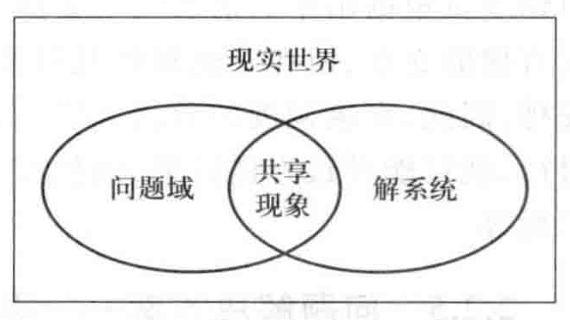
\includegraphics[width=0.3\textwidth]{img/问题域和解系统的关系.png}
\end{figure}

\subsubsection{问题域的特性}
问题域自治的规律性称为问题域特性
\begin{itemize}
    \item 问题域是自治的,它有自己的运行规律,而且这些规律不会因解系统的引入而发生改变
\end{itemize}

需额外关注的问题域特性
\begin{itemize}
    \item 间接特性
    \item 约束和假设 
    \begin{itemize}
        \item 社会性因素
    \end{itemize}
\end{itemize}

问题域特性的重要性
\begin{itemize}
    \item 要想解决问题,它就需要了解问题域特性,将解决方案和问题域特性结合起来 
    \item 要防止解系统的引入在问题域当中引发未预见的连锁反应 (例:间接特性不直接与解系统交互而引发)
\end{itemize}

\subsubsection{解系统的特性}
\begin{itemize}
    \item 解系统是问题的解决手段,并不是问题的产生地,所以解系统并不是问题域的一部分。解系统与问题域之间存在可以互相影响的接口,以实现交互活动。
    \item 用户不应该关注软件系统,而是关注问题。
    \item 开发者关注软件系统,但要学会以问题为中心思考。
\end{itemize}


\begin{figure}[H]
	\centering
	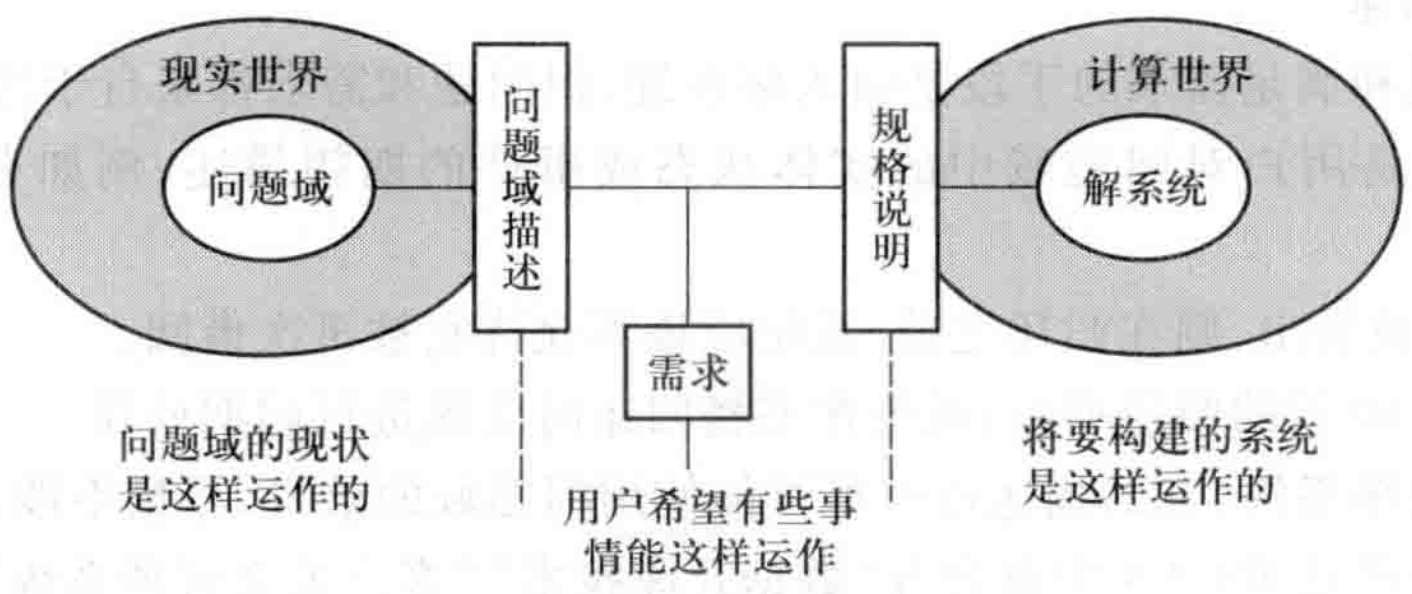
\includegraphics[width=0.55\textwidth]{img/问题域、需求、解系统、需求规格说明关系示意图.png}
\end{figure}

\subsubsection{需求规格说明}
因为解决方案以对外交互的方式定义了软件系统的功能,所以解决方案被称为软件系统的需求规格说明

IEEE将需求规格说明定义为:规定系统或部件的需求的文档,典型地包括功能需求、性能需求、接口需求、设计需求和开发标准。

\subsubsection{需求开发的形式化定义}
描述明确的问题域特性$E$,定义良好的系统行为$S$,预期的需求$R$
\begin{itemize}
    \item 需求工程的目的就是根据$E$,构建$S$,使得$E,S\mapsto R$
    \item 需求工程的困难之处:
    \begin{itemize}
        \item 不存在描述明确的$E$
        \item 不存在确定的针对$S$的评估标准$R$;
        \item $E,S \Rightarrow R$是一个创造性的过程。
    \end{itemize}
    \item 需求工程的主要工作:
    \begin{itemize}
        \item 需求开发,确定$R$
        \item 研究问题背景,描述问题域特性$E$
        \item 构建解系统,描述解系统行为$S$,使得$E,S\mapsto R$
    \end{itemize}
\end{itemize}

\subsubsection{需求工程的基本活动与实质}
\begin{figure}[H]
	\centering
	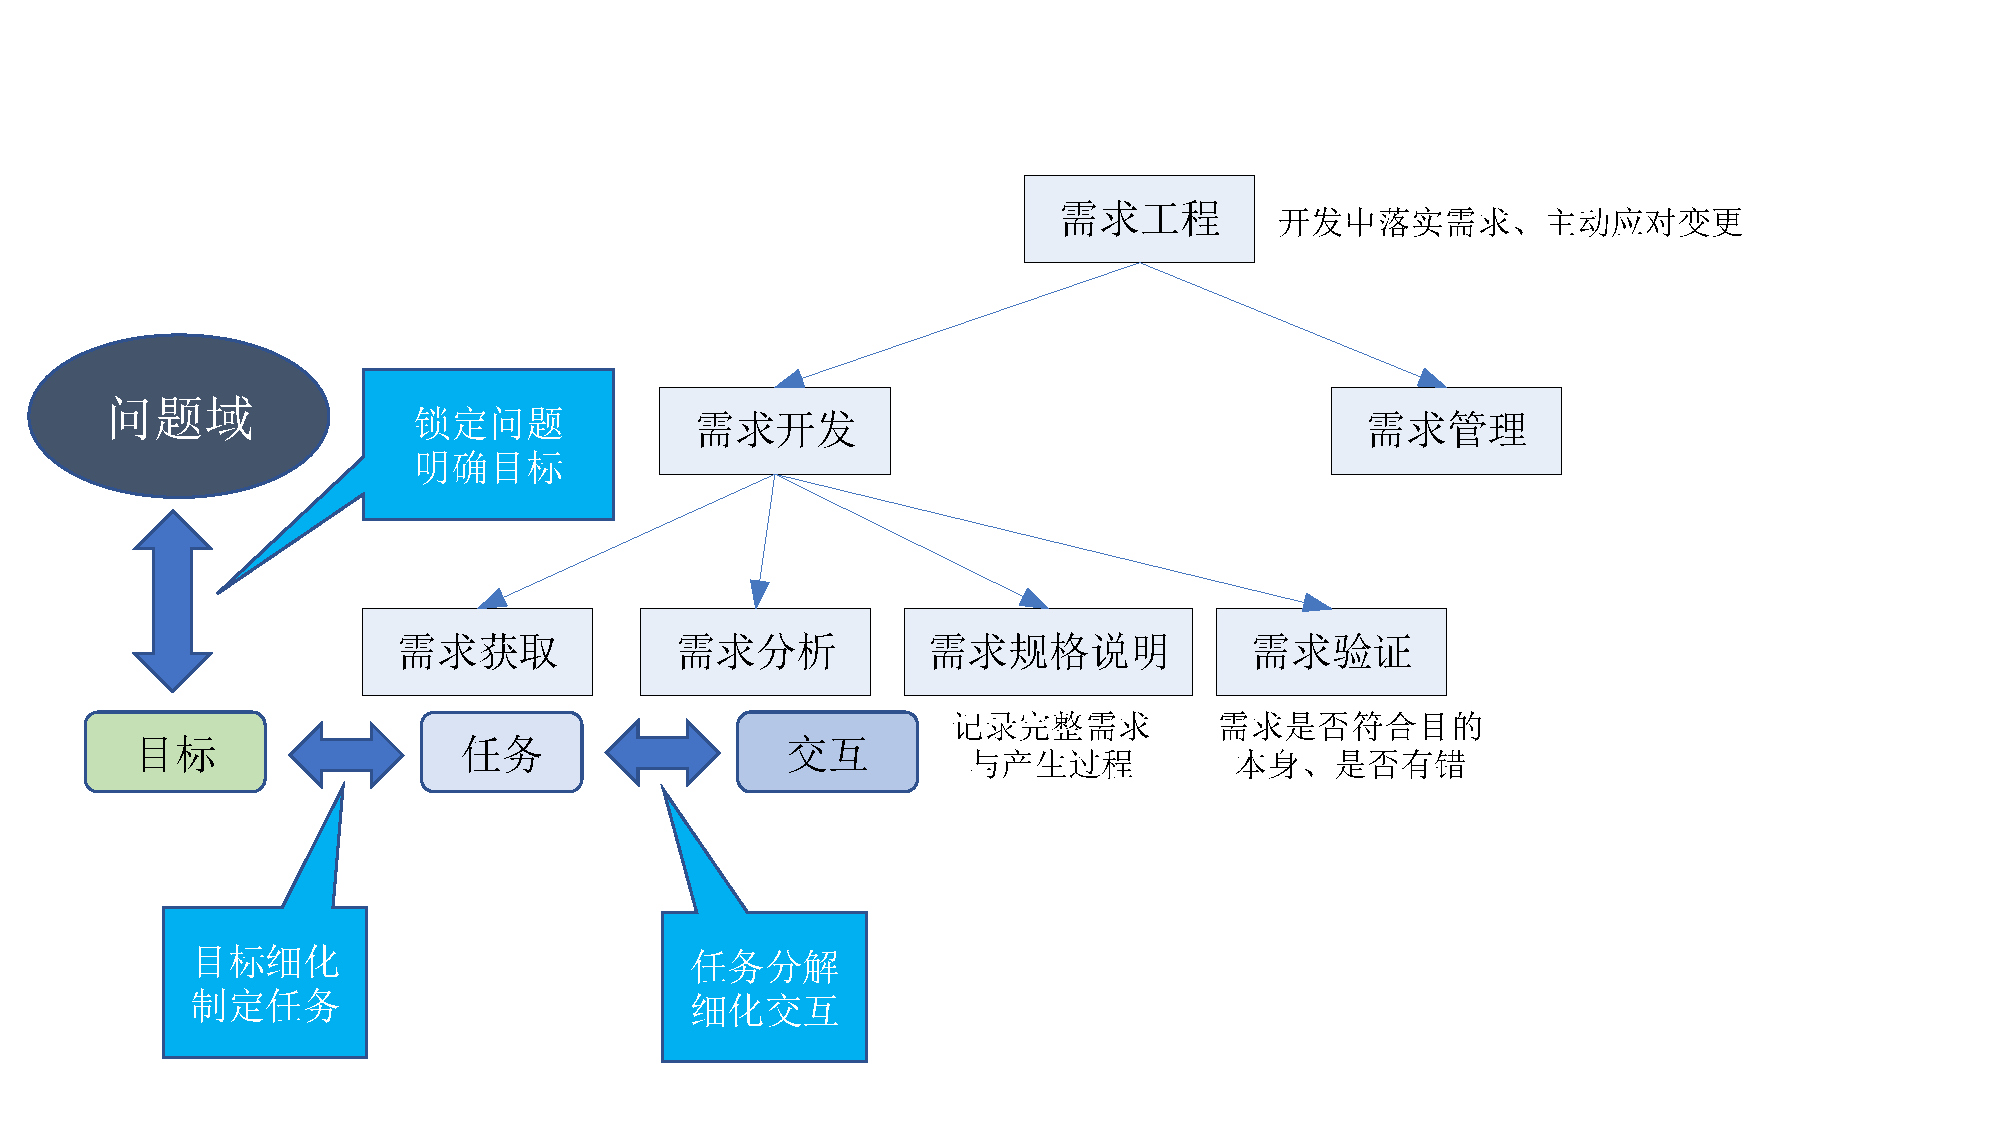
\includegraphics[width=0.8\textwidth]{img/需求工程的基本活动与实质.pdf}
\end{figure}

\subsubsection{需求工程活动的困难性}
\begin{itemize}
    \item 问题域、目标、任务、交互的相互转化是创造性的活动
    \begin{itemize}
        \item 每个案例都有其独特性,不可复用,接近于艺术
        \item 需要对问题所在的领域有着深刻的认识
        \item 需要掌握一套设计思维与辅助工具,并多多练习
    \end{itemize}
    \item 编程与设计方面的能力不能直接用于需求分析 
    \begin{itemize}
        \item 设计和编程都有构建高质量软件的共同目标,而且使用相同的概念和组织机制保证了从设计到编程的平滑过渡,所以,结构化与面向对象思维在设计领域也取得了成功
        \item 但是需求分析除了拥有构建高质量软件的目标之外,还有一个更加重要的目标是理解现实中的非技术性和社会性因素
    \end{itemize}
    \item 文档撰写、功能验证、基线管理需要丰富的开发与管理经验
\end{itemize}


\subsubsection{需求工程师:现实世界方面与技术方面的桥梁}
好的需求工程师更应该扮演好涉众代理的角色,站在涉众的立场想问题,替涉众跟踪和监控软件开发过程,保护涉众的利益
\begin{figure}[H]
	\centering
	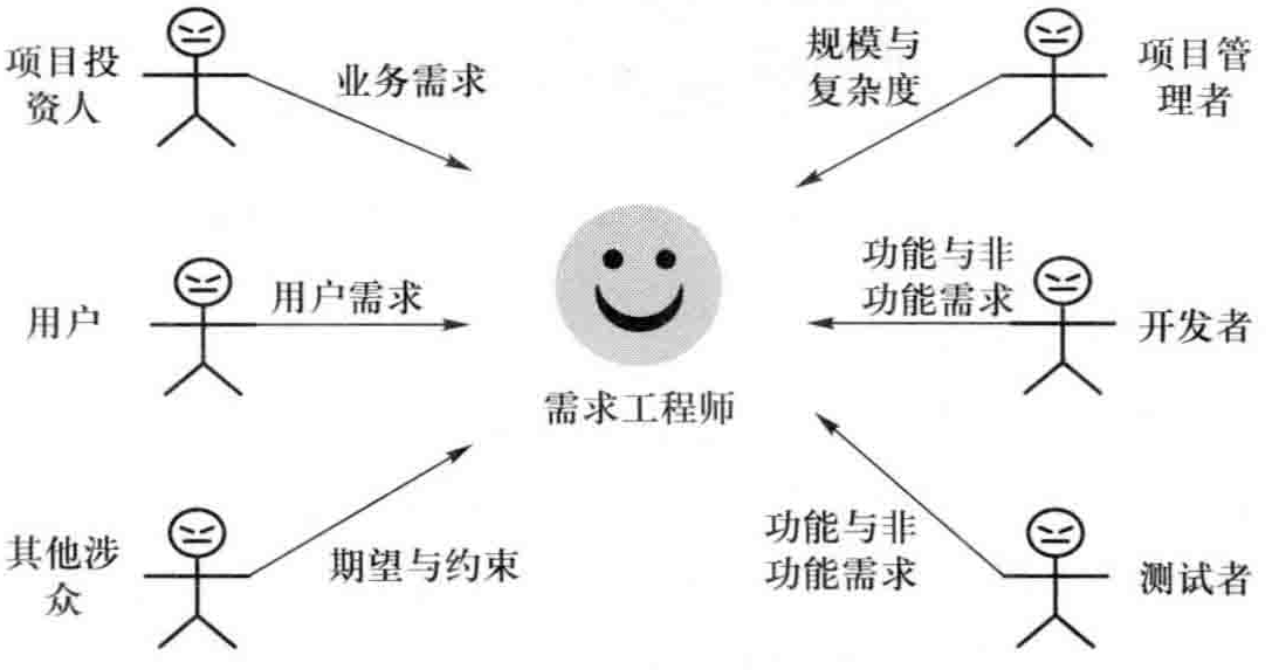
\includegraphics[width=0.6\textwidth]{img/需求工程师的桥梁作用.png}
\end{figure}

需求工程师需要具备的技能
\begin{figure}[H]
	\centering
	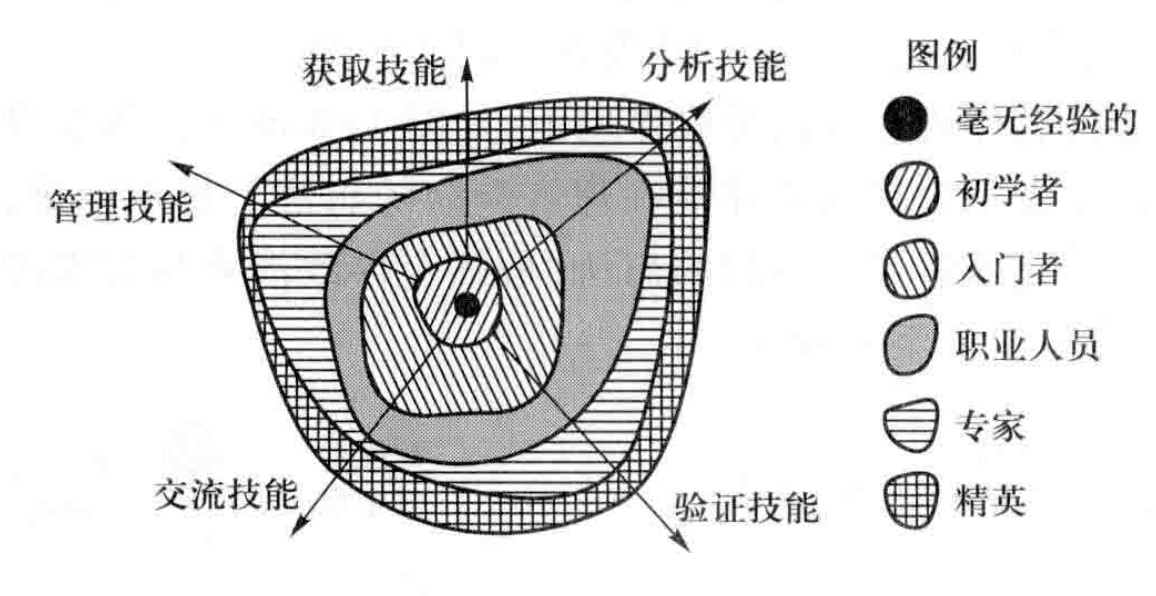
\includegraphics[width=0.55\textwidth]{img/需求工程师需要具备的技能.png}
\end{figure}

\subsection{需求的层次性}
需求是问题解决的期望,问题是可大可小的,期望自然也是可大可小的。问题和期望粒度不同的现象被称为需求的不同抽象层次。

需求最为常见的抽象层次有3层:
\begin{itemize}
    \item 业务需求:针对整个业务的期望,例如:在系统使用3个月后, 销售人员进行销售处理的工作效率应该提高20\%。
    \item 用户需求:针对具体任务的期望,例如:收银员可以使用系统完成销售处理。
    \item 系统级需求:针对用户与系统一次交互的期望,例如:在收银员请求计算已输人商品的总价时,系统应根据规则Rule1($\mbox{总价}=\sum(\mbox{价格}\times \mbox{数量} \times \mbox{折扣})$)计算总价并显示。
\end{itemize}

\begin{figure}[H]
	\centering
	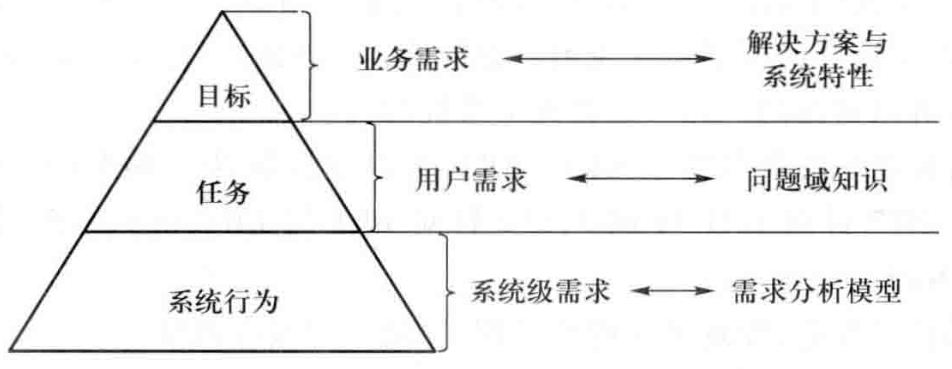
\includegraphics[width=0.55\textwidth]{img/需求的层次性.png}
\end{figure}


\subsubsection{战略问题与业务需求}
业务需求(Business Requirement,BR)是抽象层次最高的需求,是系统建立的战略出发点,表现为高层次的目标,它描述了组织为什么要开发系统。

为了满足用户的业务需求,需求工程师需要描述系统高层次的解决方案(逐一细化),定义系统应该具备的特性(System Feature, SF)
\begin{itemize}
    \item 参与各方必须要对高层次的解决方案达成一致,以建立一个共同的前景
    \item 特性说明了系统为用户提供的各项功能,它限定了系统的范围
    \item 项目的前景和范围明确了软件(某版本)的开发范畴
\end{itemize}

连锁商店销售系统业务需求示例:
\vspace{-0.25em}
{\kaishu \begin{compactitem}
    \item BR1(核心资源):在系统使用6个月后,商品积压、缺货和报废的现象减少50\%。
    \item BR2(关键业务):在系统使用3个月后,销售人员工作效率提高50\%。
    \item BR3(成本结构):在系统使用6个月后,店铺运营成本降低15\%。
    \item BR4(收入来源):在系统使用6个月后,销售额度提高20\%。
\end{compactitem}}

针对业务需求的系统特性:
\vspace{-0.25em}
{\kaishu \begin{compactitem}
    \item SF1:分析店铺商品库存,发现可能的商品积压、缺货和报废现象。BR1,BR3
    \item SF2:根据市场变化调整销售的商品。BR1,BR3,BR4
    \item SF3:制定促销手段,处理积压商品。BR1,BR3,BR4
    \item SF4:与生产厂家联合进行商品促销。BR1,BR3,BR4,CH
    \item SF5:制定促销手段进行销售竞争。BR1,BR4,CH
    \item SF6:掌握员工变动和授权情况。BR2
    \item SF7:处理商品入库与出库。BR1
    \item SF8:发展会员,提高顾客回头率。BR4,CR
    \item SF9:允许积分兑换商品和赠送吸引会员的礼品,提高会员满意度。BR3,BR4,CR
    \item SF10:帮助收银员处理销售与退货任务。BR2
\end{compactitem}}


\subsubsection{任务问题与用户需求}
用户需求是执行实际工作的用户对系统所能完成的具体任务的期望,描述了系统能够帮助用户做些什么。

用户需求是对任务的期望,基本表达方式“$\ast$$\ast$ 用户可以使用系统完成$\ast$$\ast$任务”。
\begin{itemize}
    \item 用户任务应该是有价值的活动(客户洞察),并具有较强的目标性(细化的讲故事与场景)。比如向“ATM机中插卡”就不是用户需求,因为用户不会漫无目的的插卡。
    \item 对所有的用户需求,都应该有充分的问题域知识作为支持。
\end{itemize}

用户需求的特点:
\begin{itemize}
    \item 模糊、不清晰:允许使用形容词和副词 
    \item 多特性混杂:允许混合功能和非功能性需求 
    \item 多逻辑混杂:一条用户需求所代表的任务需多次系统交互才能完成
    \begin{itemize}
        \item 需求开发阶段可视作从用户需要解决的问题到用户与系统的一系列交互的转化,此过程中用户的输入与获得的反馈不断精化,但系统本身仍被视作一个整体,留待后续设计阶段确定模块划分与结构
    \end{itemize}
\end{itemize}

例:在超市管理系统中,收银员用户的需求为:
\vspace{-0.25em}
{\kaishu \begin{compactitem}
    \item UR1:收银员可以使用系统逐一记录销售的商品。
    \item UR2:收银员可以使用系统计算商品账单并处理付款情况,账单计算需要使用促销策略。
    \item UR3:收银员可以使用系统为顾客打印收据。
    \item UR4:收银员可以使用系统退回顾客已经购买的商品。
\end{compactitem}}
  

\subsubsection{系统行为问题与系统级需求}
系统级需求是用户对系统行为的期望,一系列的系统行为联系在一起可以帮助用户完成任务,满足业务需求。

系统需求可以直接映射为系统行为(对应需求规格说明),定义了系统中需要实现的功能,描述了开发人员需要实现什么。

将用户需求转化为系统需求的过程是一个复杂的过程
\begin{itemize}
    \item 首先需要分析问题领域及其特性,从中发现问题域和计算机系统的共享知识,建立系统的知识模型;
    \item 然后将用户需求部署到系统模型当中,即定义系列的系统行为,让它们联合起来实现用户需求,每一个系统行为即为一个系统需求。
    \item 该过程就是需求工程当中最为重要的需求分析活动,又称建模与分析活动。 
\end{itemize}

系统级需求示例如下表所示
\vspace{-0.8em}
\begin{center}
    \begin{longtable}{|m{2cm}|m{11cm}|}
        \hline
        \multicolumn{1}{|c|}{需求ID}    &     \multicolumn{1}{c|}{需求描述}                                                             \\ \hline
        SR1     & 在收银员输入商品目录中已存在的商品标识时,系统显示输入商品的信息,包括ID、名称、描述、价格、特价、数量、总价。ID的规则参见DR1             \\ \hline
        \quad SR1.1   & 在收银员要求输入数量时,系统应该允许收银员输入商品的数量                                                   \\ \hline
        \quad\quad SR1.1.1 & 在收银员输入大于等于1的整数时,系统修改商品的数量为输入值,并更新显示                                            \\ \hline
        \quad\quad SR1.1.2 & 在收银员输入其他内容时,系统提示输入数量无效                                                         \\ \hline
        \quad SR1.2   & 系统应该计算并显示输入商品的总价                                                               \\ \hline
        \quad\quad SR1.2.1 & 如果存在适用(商品标识、今天)的商品特价策略(参见Rule3),系统将该商品的特价设为特价策略的特价,并计算分项总价为(特价$\times$ 数量),并将其计入特价商品总价 \\ \hline
        \quad\quad SR1.2.2 & 在商品是普通商品时,系统计算该商品分项总价为(商品的价格$\times$商品的数量),并将其计入普通商品总价                                \\ \hline
        \quad SR1.3   & 在显示商品信息0.5秒之后,系统显示已输入商品列表,并将新输入商品添加到列表中                                        \\ \hline
        SR2     & 在收银员输入商品目录中不存在的商品标识时,系统不予处理                                                    \\ \hline
        DR1     & ID是规则为……的商品条形码                                                                  \\ \hline
        Rule3   & 适用(商品标识,参照日期)的商品特价促销策略:(促销商品标识$=$商品标识)而且((开始日期早于晚于参照日期)并且(结束日期晚于等于参照日期))         \\ \hline
    \end{longtable}
\end{center}
\vspace{-3.7em}

用户需求和系统级需求在实践中经常是混淆的
\begin{itemize}
    \item 用户习惯于用户需求;
    \item 开发者需要系统级需求,但得到的往往是用户需求
    \begin{itemize}
        \item 未能得到足够信息以准确地完成设计与实现工作
        \item 需要开发者以各自方式进行假设……
    \end{itemize}
\end{itemize}

正确处理用户需求和系统级需求
\begin{itemize}
    \item 明确其不同点
    \vspace{-0.8em}
	\begin{multicols}{2}
    \begin{itemize}
        \item 用户需求:任务
        \item 系统级需求:交互
    \end{itemize}
	\end{multicols}
	\vspace{-1em}
    \item 明确建立和维护用户需求与系统级需求的关系
    \item 系统级需求的建立需要需求分析人员的创造性(建模)
\end{itemize}

\subsection{需求的分类与表述}

\subsubsection{软件需求的分类}
[IEEE 1998]将需求分成下列几个类别:
\begin{itemize}
    \item \textbf{功能需求:}和系统主要工作相关的需求,即在不考虑物理约束的情况下,用户希望系统所能够执行的活动,这些活动可以帮助用户完成任务。功能需求主要表现为系统和环境之间的行为交互。
    \item \textbf{性能需求:}系统整体或系统组成部分应该拥有的性能特征,例如CPU使用率、内存使用率等。
    \item \textbf{质量属性:}系统完成工作的质量,即系统需要在一个“好的程度”上实现功能需求,例如可靠性程度、可维护性程度等。
    \item \textbf{对外接口:}系统和环境中其他系统之间需要建立的接口,包括硬件接口、软件接口、数据库接口等等。
    \item \textbf{约束:}进行系统构造时需要遵守的约束,例如编程语言、硬件设施等。
    \item \textbf{其他:}项目中也可能会出现逻辑数据需求等其他特殊类型的需求。
\end{itemize}

\subsubsection{功能需求}
功能性需求是一个软件产品得以存在的愿意,是软件系统能够解决用户问题和产生价值的基础,也是整个软件开发工作的基础。

通常一个软件系统的绝大部分需求都是功能需求,但在比例上功能需求有可能占所有需求的90\%以上。

在大规模软件系统中,因为其功能需求比较复杂,所以它是最需要按照了个抽象层次进行展开的需求类别,也就是说功能需求的开发要围绕“目标$\rightarrow$任务$\rightarrow$交互”(BR(SF)$\rightarrow$UR$\rightarrow$SR)的路线进行,对“目标”、“任务”和“交互”3个概念的关注是功能需求开发的重中之重。

\subsubsection{性能需求}
[IEEE 1990]对性能的定义是:一个系统或其组成部分在限定的约束下,完成其指定功能的程度,如速度、精确性和内存使用程度等。性能需求定义了系统必须多好和多快地完成专门的功能。

常见的性能需求包括以下几种
\begin{itemize}
    \item 速度(Speed),系统的响应时间。PR1:所有的用户查询都必须在10秒内完成。
    \item 容量(Capacity),系统所能存储的数据量。PR2:系统应该能够存储至少10万条销售记录。
    \item 吞吐量(Throughput),系统在连续的时间内完成的事务数量。PR3:解释器每分钟应该至少解析5000条没有错误的语句。
    \item 负载(Load),系统可以承载的并发工作量。PR4:系统应该允许200个用户同时进行正常的工作。
    \item 实时性(Time-Critical),严格的实时要求。PR5:监测到病人异常后,监控器必须在0.5秒内发出警报。
\end{itemize}

\subsubsection{质量属性}
\begin{itemize}
    \item 系统为了满足规定的及隐含的所有要求而需要具备的要素称为质量(包含性能需求) 
    \item 质量属性是为了度量质量要素而选用的特征 
    \item 质量模型就是能够为质量需求的描述和评价提供工作基础的特征集及特征之间的联系 
\end{itemize}

常见的质量属性示例:
\begin{itemize}
    \item 可靠性(Reliability):在规格时间间隔内和规定条件下,系统或部件执行所要求能力的能力
    \begin{itemize}
        \item QR1:在进行数据的下载和上传中,如果网络故障,系统不能出现故障
        \begin{itemize}
            \item QR1.1:分店子系统应该检测到故障,并尝试重新连接网络3次,每次15秒
        \end{itemize}
    \end{itemize}
    \item 可用性(Availability):软件系统在投入使用时可操作和可访问的程度或能实现其指定系统功能的概率
    \begin{itemize}
        \item QR2:系统的可用性要达到98\%
    \end{itemize}
    \item 安全性(Security):软件阻止对其程序和数据进行未授权访问的能力,未授权的访问可能是有意,也可能是无意的
    \begin{itemize}
        \item QR3:收银员只能查看,不能修改、删除VIP顾客的信息
    \end{itemize}
    \item 可维护性(Maintainability):软件系统或部件能修改以排除故障、改进性能或其他属性或适应变更了的环境的容易程度,包括可修改性(Modifiability)和可扩展性(Extensibility)
    \begin{itemize}
        \item QR4:如果系统要增加新的特价类型,要能够在2个人月内完成。
    \end{itemize}
    \item 可移植性(Portability):可移植性指系统或部件能从一种硬件或软件环境转换至另外一种环境的特性
    \begin{itemize}
        \item QR5:服务器要能够在1人月内从Windows7操作系统更换到Solaris 10操作系统。
    \end{itemize}
    \item 易用性(Usability):与用户使用软件所花费的努力及其对使用的评价相关的特性。
    \begin{itemize}
        \item QR6:使用系统1个月的收银员进行销售处理的效率要达到10件商品每分钟
    \end{itemize}
\end{itemize}

\begin{figure}[H]
	\centering
	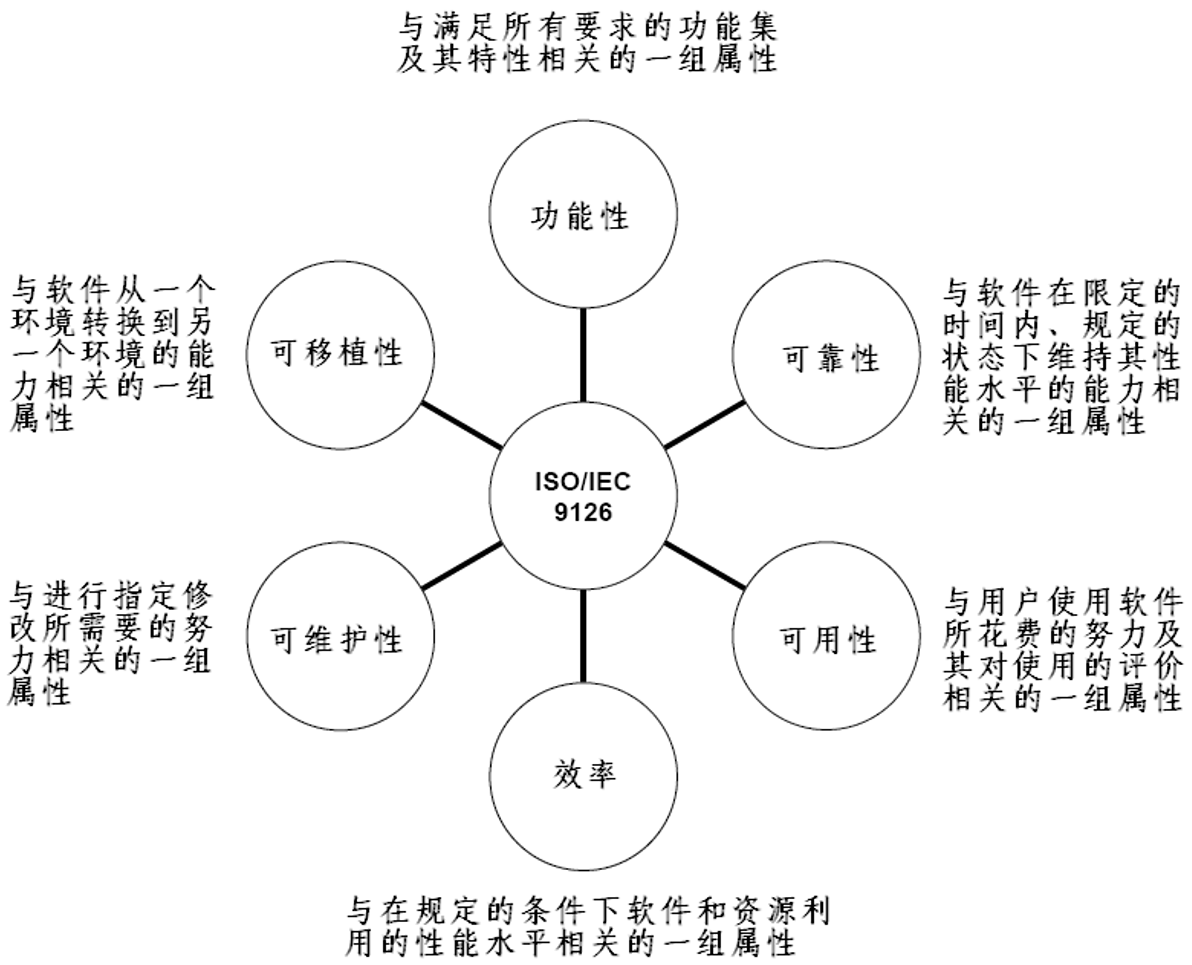
\includegraphics[width=0.6\textwidth]{img/质量属性举例.png}
\end{figure}

\subsubsection{对外接口}
对系统之间的软硬件接口需要说明以下内容
\vspace{-0.8em}
\begin{multicols}{3}
\begin{itemize}
    \item 接口的用途
    \item 接口的输入输出
    \item 数据格式
    \item 命令格式
    \item 异常处理要求
\end{itemize}
\end{multicols}
\vspace{-1em}

对外接口需求规格片段
{\kaishu 
\vspace{-0.8em}
\begin{multicols}{2}
    \columnseprule=0.8pt
    IR1:与地图API的接口:定位用户与商户的位置 \\
    参数:手机GPS定位坐标。\\
    返回值:在地图的定位,并基于此给出最近的商家。
    
    IR2:支付宝接口:订单生效应允许通过支付宝付款。\\
    参数:商家支付宝号,顾客支付宝号,应付款额。\\
    返回值:支付成功或支付失败状态。
\end{multicols}
\vspace{-1em}}

用户界面在有些情况下也会被视为系统的对外接口,被作为一种重要的需求。但[CMU/SEI1991]认为,和其他需求相比,用户的界面更经常发生变化,进而影响需求的稳定性,所以[CMU/SEI1991]建议如果将用户界面作为需求一部分的话,一定要进行单独处理和组织。通常,对于人机交互复杂的系统使用单独的人机交互设计文档记录用户界面需求,否则可以将其作为需求文档的一部分进行记录。

\subsubsection{约束}
总体上限制了开发人员设计和构建系统时的选择范围 
\begin{itemize}
    \item 系统开发及运行的环境:包括目标机器、操作系统、网络环境、编程语言、数据库管理系统等
    \item 问题域内的相关标准(商业模式评估):包括法律法规、行业协定、企业规章等
    \item 商业规则(商业模式设计):用户在任务执行中的一些潜在规则也会限制开发人员设计和构建系统的选择范围
\end{itemize}

进入21世纪以来,基于web的产品发展,软件对周围环境的要求越来越突出,尤其是:
\begin{itemize}
    \item 商业规则:目标、规则、边界值与异常情况处理
    \item 法规与行业规范:新业务与灰色地带,利用违规内容抹黑竞争对手
    \item 社会性因素:宗教信仰、价值取向、流行风潮等
\end{itemize}

规则描述样式与示例
\vspace{-0.8em}
\begin{center}
    \begin{longtable}{|m{0.8cm}<{\centering}|m{6.5cm}|m{6.5cm}|}
        \hline
        \multicolumn{1}{|c|}{类别}    &     \multicolumn{1}{c|}{描述样式}    &    \multicolumn{1}{c|}{示例}                                                   \\ \hline
        术语                  & {[}限定词{]}\textless{}名词/业务术语\textgreater{}是指\textless{}文字描述\textgreater{}                                                            & Rule2:退货是指顾客在一个时间点上凭之前1周内的购物发票,退回其中一项或多项商品的行为;                        \\ \hline
        \multirow{2}{*}{事实} & {[}限定词{]}\textless{}名词/业务术语1\textgreater{}{[}条件限定{]}必须|可能\textless{}动词或动词短语\textgreater{}{[}限定词{]}\textless{}名词/业务术语2\textgreater{} & Rule3:同样的商品在不同的时期内可能有不同的价格;                                           \\ \cline{2-3} 
                            & \textless{}名词/业务术语1\textgreater{}的特征有\textless{}名词/业务术语2\textgreater{}                                                              & Rule4:每件商品都有一个条形码                                                     \\ \hline
        \multirow{2}{*}{约束} & {[}限定词{]}\textless{}名词/业务术语\textgreater{}必须满足\textless{}条件\textgreater{}                                                            & Rule5:商品条形码符合EAN-13标准                                                 \\ \cline{2-3} 
                            & \textless{}名词/业务术语\textgreater{}必须/不能\textless{}动词或动词短语\textgreater{}\textless{}条件\textgreater{}                                    & Rule6:商品特价的折扣率不能超过50\%                                                \\ \hline
        推导                  & \textless{}名词/业务术语\textgreater{}的计算方式为\textless{}数学计算表达式\textgreater{}                                                              & Rule7:普通商品项总价 = 价格×数量                                                 \\ \hline
        推理                  & 如果\textless{}条件1\textgreater{}{[}和/或者\textless{}条件2\textgreater{}…{]},那么\textless{}结论\textgreater{}                                 & Rule8:如果销售日期在一周之前,或者销售是用积分付款的,或者销售的非积分付款余额已经不足以支付商品退款额,那么该商品就属于不可退货商品 \\ \hline
    \end{longtable}
\end{center}
\vspace{-3.7em}

\subsubsection{其他需求}
\begin{itemize}
    \item 安装需求(例如OR1)、培训需求(OR2)、数据需求等
    
    {\kaishu 
    OR1:在安装系统时,要初始化用户、商品库存等重要数据。\\
    OR2:系统投入使用时,需要对用户进行1个星期的集中培训。
    }
    \item 如果在功能需求中没有描述数据内容(例如SR3),就需要补充描述数据信息(例如DR1$\sim$DR2)。
    
    {\kaishu
    SR3:在收银员输入商品标识时,系统显示商品信息,商品信息参见DR1、DR2;\\
    DR1:ID是规则为……的商品条形码;\\
    DR2:商品信息包括:ID、名称、描述、价格、特价、数量、总价
    }
\end{itemize}


	\section{需求工程过程}

\subsection{概述}
过程是一组相关活动的集成,通过这些活动的执行,可以完成一项任务或者达到一个目标。

需求工程过程是系统开发当中需求开发活动的集成,它的模版是产生一个能够在用户环境下解决用户业务问题的系统方案。

需求工程过程可能会表现出极大的差异,但是除了少数情况之外,主要的需求工程活动是比较固定的。

\begin{figure}[H]
	\setcounter{subfigure}{0}
	\centering
	\vspace{-0.5em}	
	\subfloat{
	\begin{minipage}[c]{0.4\linewidth}
	\centering
	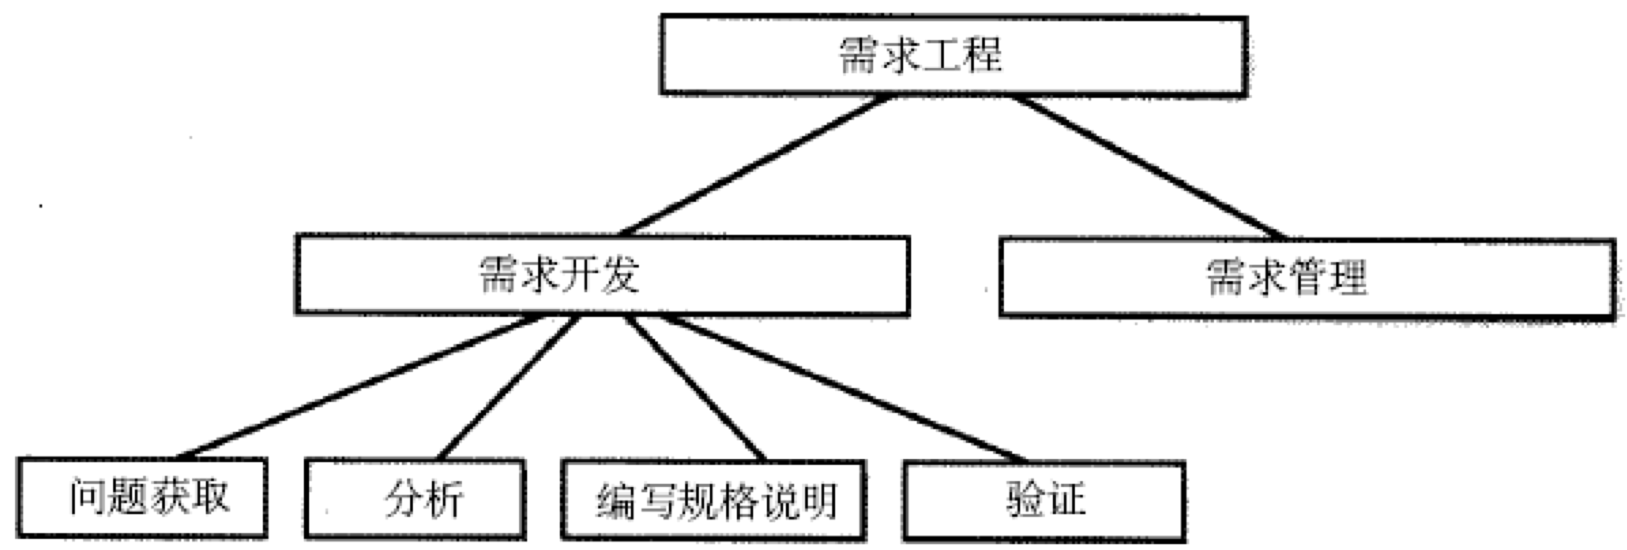
\includegraphics[width=\linewidth]{img/需求工程过程1.png}
	\end{minipage}
    }
	\subfloat{
	\begin{minipage}[c]{0.57\linewidth}
	\centering
	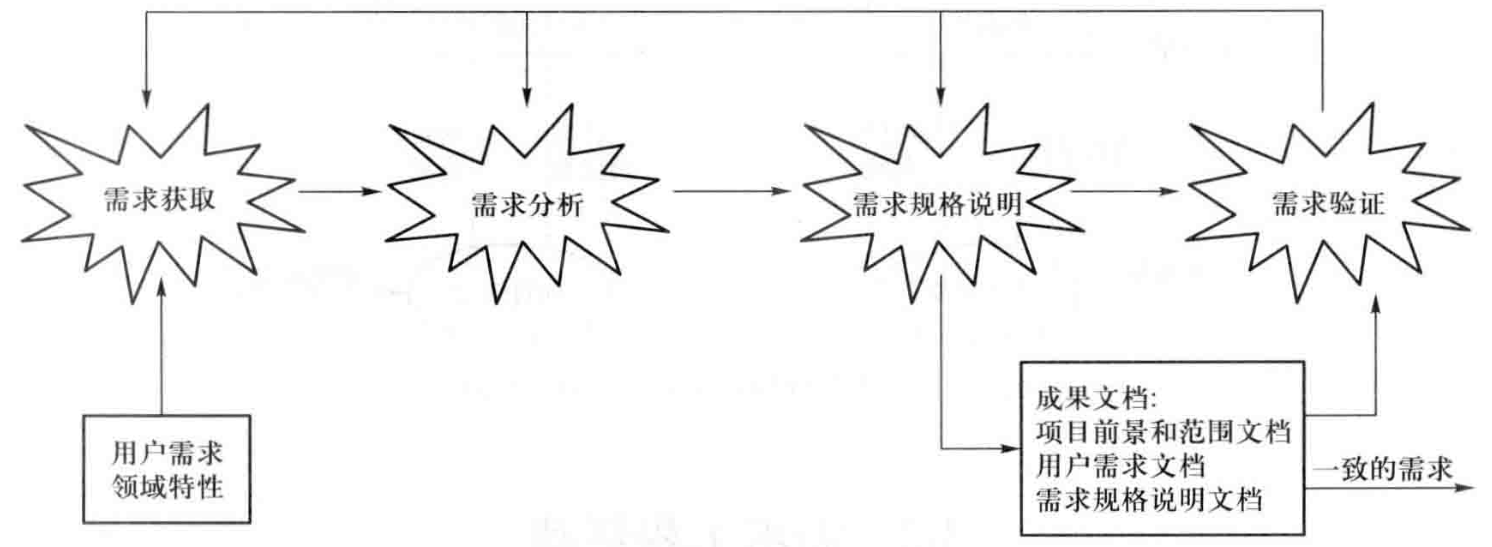
\includegraphics[width=\linewidth]{img/需求工程过程2.png}
	\end{minipage}
	}
	\centering
	\vspace{-1em}
\end{figure}

\subsection{需求工程的基本活动}
\begin{itemize}
    \item \textbf{需求获取:}系统原始需要
    \begin{itemize}
        \item 研究应用环境,分析系统涉众,了解已有问题,建立系统目标,获取业务细节,生成用户需求
    \end{itemize}
    \item \textbf{需求分析:}保证需求完整性与一致性(贯穿整个过程)
    \begin{itemize}
        \item 将目标、功能与约束映射为系统行为,建立系统模型并分析(信息的细化与隐藏联系、假设的显式化),识别并修复不一致缺陷,发现并弥补遗漏的需求
    \end{itemize}
    \item \textbf{需求规约:}将分析过的需求与系统行为明确并文档化
    \begin{itemize}
        \item 自然语言$+$模型语言(UML)
    \end{itemize}
    \item \textbf{需求验证:}保证需求分档的正确性、一致性、完整性
    \begin{itemize}
        \item 最终产物为所有涉众一致同意的需求规约,是后续开发的基础
    \end{itemize}
    \item \textbf{需求管理:}持续(时间、开发活动)管理需求基线
    \begin{itemize}
        \item 跟踪后续阶段中的需求实现与变更,确保正确的理解与实现
    \end{itemize}
\end{itemize}

\subsection{需求开发过程是迭代和并发的}
\begin{figure}[H]
	\setcounter{subfigure}{0}
	\centering
	\vspace{-2em}	
	\subfloat{
	\begin{minipage}[c]{0.48\linewidth}
	\centering
	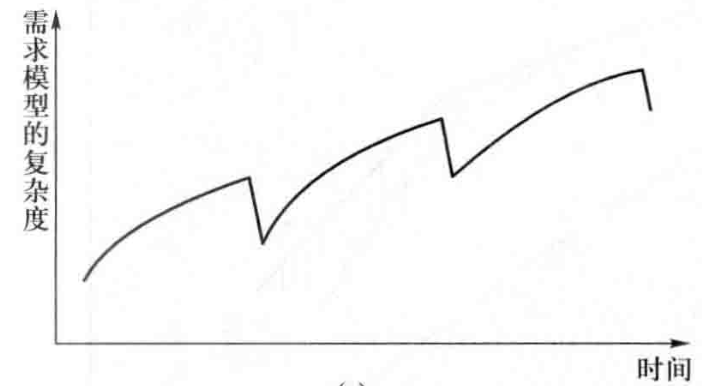
\includegraphics[width=0.8\linewidth]{img/需求开发过程是迭代和并发的1.png}
	\end{minipage}
    }
	\subfloat{
	\begin{minipage}[c]{0.48\linewidth}
	\centering
	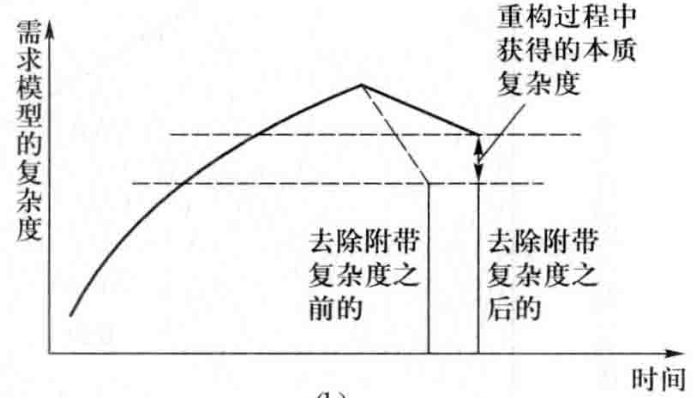
\includegraphics[width=0.8\linewidth]{img/需求开发过程是迭代和并发的2.png}
	\end{minipage}
	}

    \subfloat{
        \begin{minipage}[c]{0.55\linewidth}
        \centering
        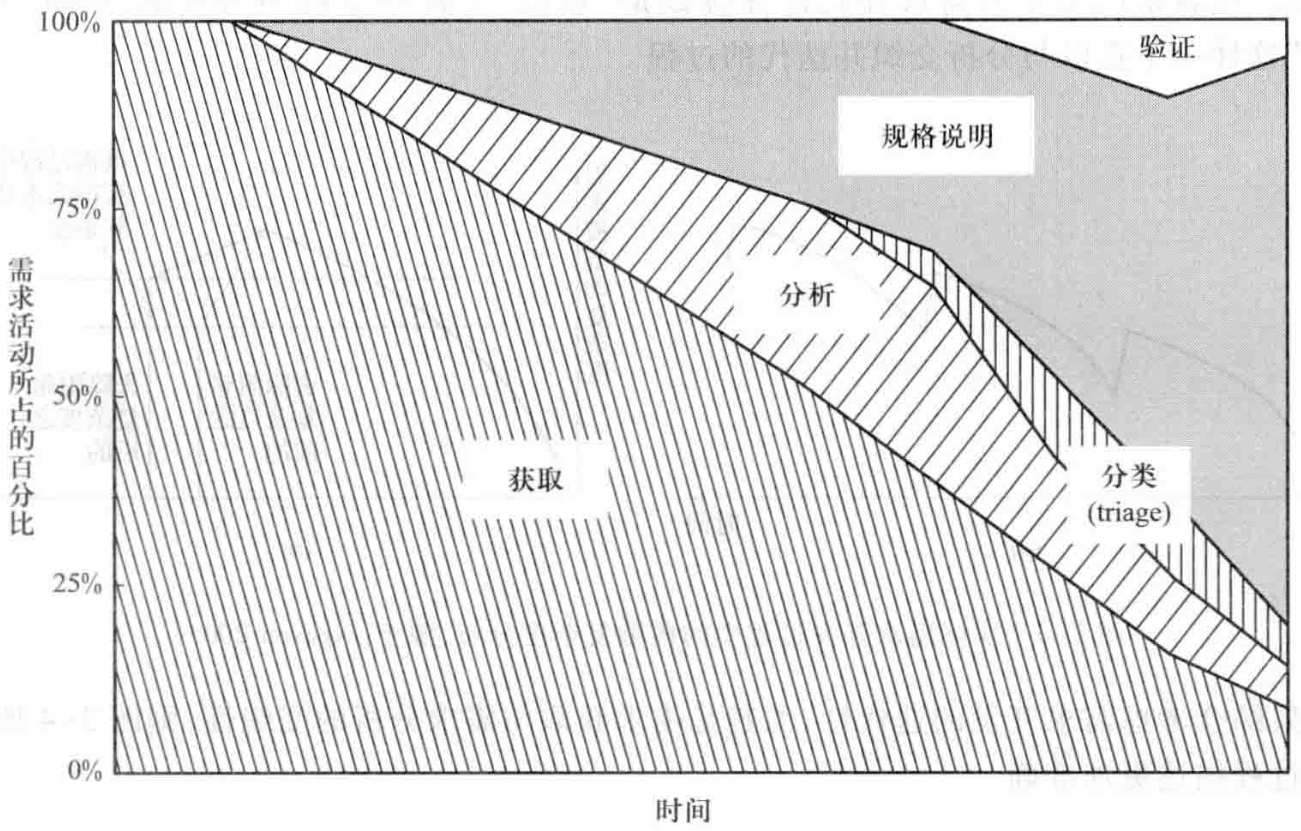
\includegraphics[width=0.97\linewidth]{img/需求开发过程是迭代和并发的3.png}
        \end{minipage}
    }
	\centering
	\vspace{-1em}
\end{figure}


\subsection{实践方法的应用}

\vspace{-0.8em}
\begin{center}
    \begin{longtable}{|m{2cm}|m{3.5cm}|m{3.2cm}|m{4.6cm}|}
        \hline
        \multicolumn{1}{|c|}{活动} & \multicolumn{1}{c|}{有效实践}   & \multicolumn{1}{c|}{内容}          & \multicolumn{1}{c|}{技术及方法}                \\ \hline
        \multirow{15}{*}{需求获取}   & 定义项目前景                      & 定义项目前景                           & 问题分析、目标分析、业务过程分析、分析非功能需求、定义系统边界、编写前景与范围文档 \\ \cline{2-4} 
                                 & 控制项目范围                      & 控制项目范围                           & 同上                                        \\ \cline{2-4} 
                                 & \multirow{3}{*}{实现用户价值}     & 涉众识别                             & 先膨胀后收缩、检查列表、涉众网络                          \\ \cline{3-4} 
                                 &                             & 涉众描述                             & 涉众的描述特征                                   \\ \cline{3-4} 
                                 &                             & 涉众评估                             & 优先级评估、风险评估、共赢分析                           \\ \cline{2-4} 
                                 & \multirow{2}{*}{促进用户参与}     & 涉众代表选择                           & 代表采样、使用用户替代源                              \\ \cline{3-4} 
                                 &                             & 参与策略制定                           & 制定参与基本策略、敏捷方法---用户参与                      \\ \cline{2-4} 
                                 & \multirow{3}{*}{识别并使用各种需求源} & 涉众分析                             & 涉众分析的各种方法(如前述)                            \\ \cline{3-4} 
                                 &                             & 硬数据采样                            & 硬数据采样                                     \\ \cline{3-4} 
                                 &                             & 需求重用                             &                                           \\ \cline{2-4} 
                                 & \multirow{4}{*}{有效的获取需求}    & 建立有效交流机制                         & 建立合作关系,维护交流气氛,利用适当的交流途径、交流方式              \\ \cline{3-4} 
                                 &                             & \multirow{3}{*}{\begin{tabular}[c]{@{}l@{}}正确使用需求获取\\ 方法\end{tabular}}      & 面谈/调查问卷/群体面谈、头脑风暴                         \\ \cline{4-4} 
                                 &                             &                                  & 原型                                        \\ \cline{4-4} 
                                 &                             &                                  & 观察、民族志、文档分析/需求重用/需求剥离                     \\ \cline{2-4} 
                                 & 收集和组织需求获取的结果                & 建立收集和组织需求结果的机制                   & 用例/场景模型                                   \\ \hline
        \multirow{6}{*}{需求分析}    & \multirow{3}{*}{为需求建模}      & \multirow{2}{*}{\begin{tabular}[c]{@{}l@{}}通过建模手段明确和\\理解需求信息\end{tabular}} & 结构化分析模型                                   \\ \cline{4-4} 
                                 &                             &                                  & 面向对象分析模型                                  \\ \cline{3-4} 
                                 &                             & 使用多种手段从多角度建模相同的内容                & 多视点方法、Wieringa框架、Zachman框架                \\ \cline{2-4} 
                                 & 在合适的层次上描述需求                 & 需求细化                             &                                           \\ \cline{2-4} 
                                 & 唯一地标识每一条需求                  & 需求细化                             &                                           \\ \cline{2-4} 
                                 & 划分需求的优先级                    & 确定需求优先级                          & 累计投票、区域划分、Top-N、数据量化                      \\ \hline
        \multirow{4}{*}{需求规格说明}  & 使用模板                        & 使用需求文档模板                         & {[}IEEE 1998{]}的模板                        \\ \cline{2-4} 
                                 & \multirow{3}{*}{进行良好的写作}    & 综合使用各种描述手段                       & 形式化、半形式和非形式化描述                            \\ \cline{3-4} 
                                 &                             & \multirow{2}{*}{学习有效的写作实践}       & 写作技巧、优秀需求规格说明文档特性                         \\ \cline{4-4} 
                                 &                             &                                  & 需求写作事项、优秀需求的特性                            \\ \hline
        需求验证                     & 验证需求                        & 使用有效方法进行需求的验证和确认                 & 需求评审、原型与模拟、开发测试用例、用户手册编制、利用跟踪关系、自动化分析     \\ \hline
        \multirow{3}{*}{需求管理}    & 建立和维护需求基线                   & 建立和维护需求基线                        & 配置管理、状态维护                                 \\ \cline{2-4} 
                                 & 进行变更控制                      & 进行变更控制                           & 变更控制过程、变更控制事项(策略)                         \\ \cline{2-4} 
                                 & 建立需求跟踪信息                    & 建立需求跟踪信息                         & 低端/高端的需求跟踪使用、需求依赖                         \\ \hline
    \end{longtable}
\end{center}
\vspace{-3.7em}



	\section{确定项目的前景与范围}

\subsection{引言}

\subsubsection{为什么要确定项目的前景和范围}
在看待现实世界时:世界是复杂的,从不同的角度观察(目的与条件),会看到不同的内容(抽象与映射)。所以会有两个问题:
\begin{itemize}
    \item 如何保证项目涉众以符合项目需要的角度描述现实世界?
    \item 描述哪些事物和事件才会尽可能的符合项目的需要?
\end{itemize}

因此需要
\begin{itemize}
    \item 定义项目前景:所有的涉众都从共同认同的项目前景出发,理解和描述问题域及需求
    \item 定义项目范围:范围内的事物和事件是描述的目标
\end{itemize}

\subsubsection{确定项目前景和范围的关键}
确定项目前景和范围的关键是定义业务需求和能够满足需求的高层解决方案,包括:
\vspace{-0.8em}
	\begin{multicols}{3}
        \begin{itemize}
            \item 业务目标、目的
            \item 高层业务功能
            \item 每个高层业务功能所关联的高层数据
            \item 每个功能相关的项目涉众
            \item ……
        \end{itemize}
	\end{multicols}
\vspace{-1em}
如果存在不同业务需求之间的冲突,那么在确定项目前景和范围阶段必须予以解决

\subsubsection{问题概述}
确定项目的前景与范围,就是确定项目的问题、目标、特性
\begin{itemize}
    \item (业务需求)问题:组织的战略目标、利益分配、政策规划、业务流程等高层问题
    \item 目标:问题的反面,用户的期望
    \item 系统特性(解决问题的方向):选定的、针对目标的解决方案所需要具备的功能特征,通常内聚于一个目标与任务,反映系统与外界一次有价值的完整互动过程(用户)
\end{itemize}

针对项目的复杂程度,针对“范围”可以采用的分析手段由浅到深依次为问题分析、目标分析、业务过程分析
\begin{itemize}
    \item 问题与目标明确$\rightarrow$问题分析$\rightarrow$用例图/上下文图
    \item 目标之间存在较为复杂的关系$\rightarrow$目标分析$\rightarrow$目标模型与目标实现
    \item 目标、特性之间存在紧密的联系$\rightarrow$业务过程分析$\rightarrow$UML活动图
    \item 分析过程越复杂,分析结果的形式化程度越高,变更的成本也越大
\end{itemize}

此外,还需要分析非功能需求,定义系统边界,生成前景与范围文档

\subsection{问题分析}

\subsubsection{获取问题}
问题分析的前提是获取问题,这可以通过收集背景资料或与涉众沟通来实现。

连锁商店获取问题示例:
\vspace{-0.25em}
{\kaishu \begin{compactitem}
    \item P1:手工作业销售迟缓,效率不高。
    \item P2:商店的商品品种太多,无法准确掌握库存。
    \item P3:成本不够低,导致竞争力不强,盈利水平不够。
    \item P4:顾客不够多,销售额不高,盈利水平不够。
\end{compactitem}}

\subsubsection{问题解决方案描述}
\vspace{-0.5em}
\begin{center}
    \begin{longtable}{|Wc{2cm}|Wc{1.5cm}|m{11cm}|}
        \hline
        \multicolumn{2}{|c|}{\textbf{要素}}                          & \multicolumn{1}{c|}{\textbf{内容}}                                                \\ \hline
        \multicolumn{2}{|c|}{ID}                                   & \multicolumn{1}{c|}{P2}                                                          \\ \hline
        \multicolumn{1}{|c|}{\multirow{3}{*}{解决方案1}} & 方案描述        & 准确的库存管理,记录入库和出库,提供实时的库存分析数据,可以及时地发现可能的积压、缺货、报废现象。           \\ \cline{2-3} 
        \multicolumn{1}{|c|}{}                       & 业务优势        & 及时发现积压、缺货与报废,可以尽早处置。                                        \\ \cline{2-3} 
        \multicolumn{1}{|c|}{}                       & 代价          & 对积压、缺货的预测可能不准确,会因此而产生代价。                                    \\ \hline
        \multicolumn{1}{|c|}{\multirow{3}{*}{解决方案2}} & 方案描述        & 制定促销策略,处置可能的积压和报废商品。                                        \\ \cline{2-3} 
        \multicolumn{1}{|c|}{}                       & 业务优势        & 通过促销,可以减少积压和报废商品带来的损失。                                      \\ \cline{2-3} 
        \multicolumn{1}{|c|}{}                       & 代价          & 促销本身会产生代价。                                                  \\ \hline
        \multicolumn{1}{|c|}{\multirow{3}{*}{解决方案3}} & 方案描述        & 根据过去的销售情况预测未来的销售数据,并据此调整商品购买时机和数量。                          \\ \cline{2-3} 
        \multicolumn{1}{|c|}{}                       & 业务优势        & 可以做到成本最小化。                                                  \\ \cline{2-3} 
        \multicolumn{1}{|c|}{}                       & 代价          & 如果预测不准确,产生较多的缺货现象会降低顾客满意度。                                  \\ \hline
        \multicolumn{1}{|c|}{\multirow{3}{*}{解决方案4}} & 方案描述        & 对积压、报废和缺货现象比较频繁的商品进行调整。将总是积压和报废的商品调整出销售目录,为总是缺货的商品引入新的同类商品。 \\ \cline{2-3} 
        \multicolumn{1}{|c|}{}                       & 业务优势        & 可以比较长远地解决积压、缺货、报废现象。                                        \\ \cline{2-3} 
        \multicolumn{1}{|c|}{}                       & 代价 & 无     \\\hline
    \end{longtable}
\end{center}
\vspace{-3.7em}

\subsubsection{面向对象边界描述:用例图}
\vspace{-1em}
\begin{figure}[H]
	\centering
	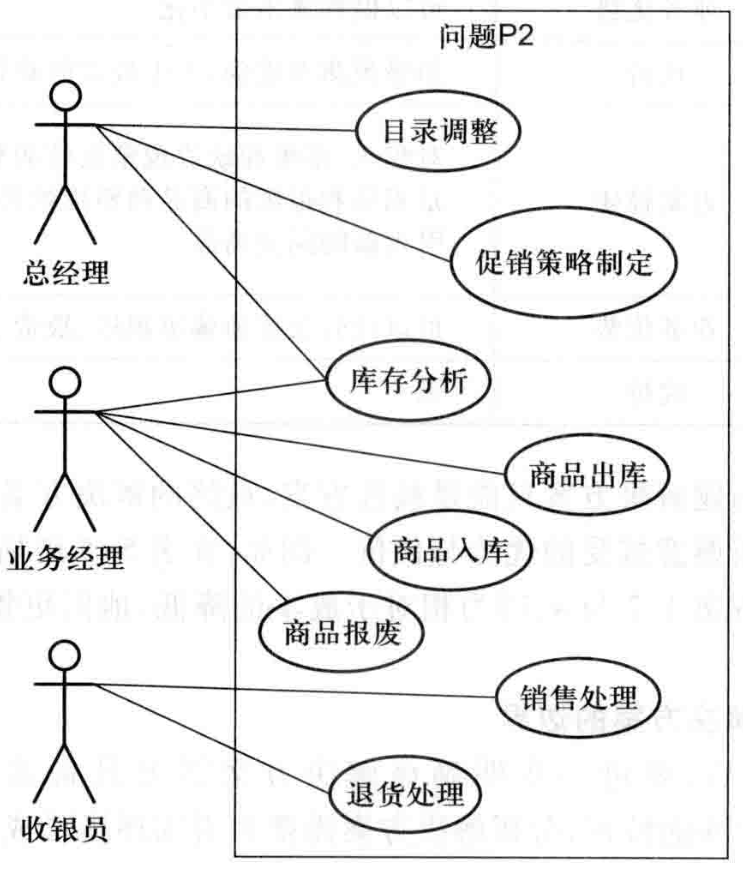
\includegraphics[width=0.32\textwidth]{img/问题P2的用例图.png}
\end{figure}
\vspace{-1em}


\subsection{目标分析}

\subsubsection{“目标”概念——面向目标的需求工程方法}
面向目标的需求工程方法是一种正式定义“目标”概念,并以此为基础开展需求工程活动的方法。也就是说,面向目标需求工程方法中的“目标” 概念是被明确定义的,有相应的方法和技术负责它的解释和使用。

面向目标的需求工程方法是指向整个需求工程的,对当今需求工程方法和技术的影响比较普遍,但是它的核心作用表现在前期需求阶段—一项目前景与范围定义活动。

\subsubsection{目标模型}

\paragraph{目标}~{} \par
日标是系统被开发的目的
\begin{itemize}
    \item 它有着明确的定义方式 
    \item 每个日标都拥有一些特征属性,常见的有类型、名称、说明、优先级、可行性和效用等
\end{itemize}

\begin{figure}[H]
	\centering
	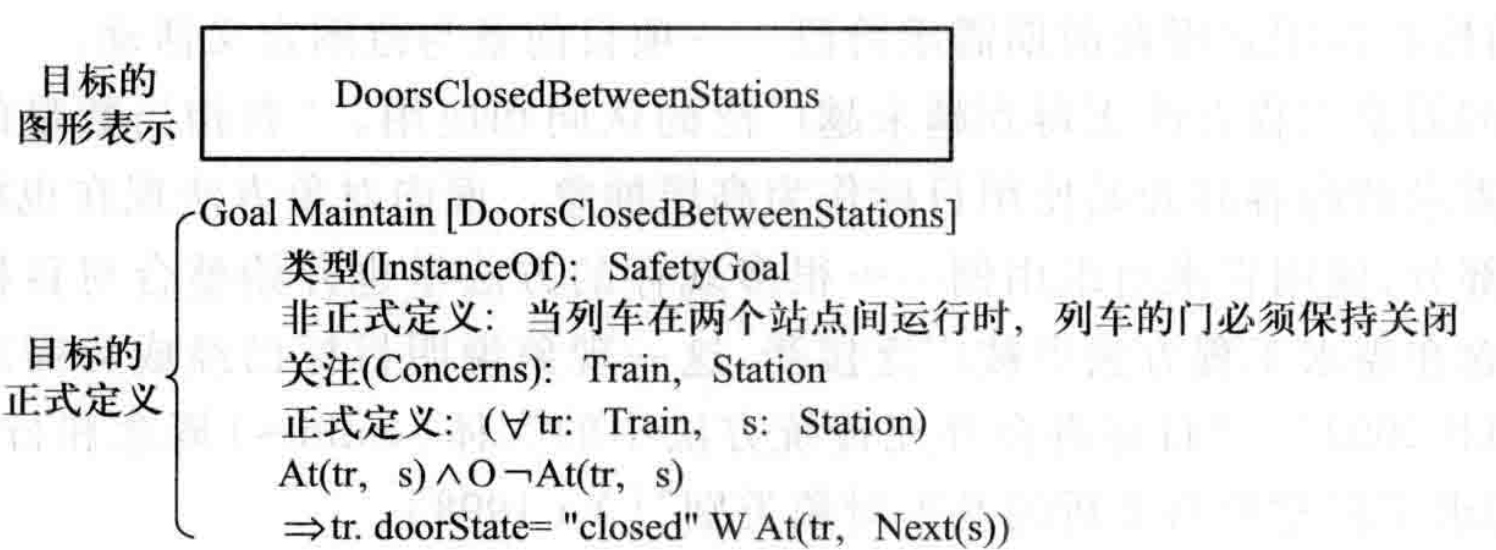
\includegraphics[width=0.7\textwidth]{img/KAOS对目标的描述.png}
    \caption*{KAOS对目标的描述}
\end{figure}
\vspace{-1em}

时序逻辑常用操作符
\begin{table}[H]
    \centering
    \begin{tabular}{|c|c|c|}
    \hline
    操作符 & 用法    & 含义                 \\ \hline
    $\bigcirc$   & $\bigcirc$Q    & 在下一个状态中Q必须为真       \\ \hline
    {\Large $\bullet$}   & {\Large $\bullet$}Q    & 在前一个状态中Q必须为真       \\ \hline
    $\lozenge$   & $\lozenge$Q    & Q终将在未来的某个时间点上为真    \\ \hline
    $\blacklozenge$   & $\blacklozenge$Q    & 过去的某个时间上Q曾经为真      \\ \hline
    $\square$   & $\square$Q    & 在所有后续路径中,Q必须始终为真   \\ \hline
    $\blacksquare$   & $\blacksquare$Q    & 在过去的路径中,Q必须始终为真    \\ \hline
    U   & P\;U\;Q & P必须一直为真直到将来的某一点Q为假 \\ \hline
    W   & P\;W\;Q & P必须一直为真直到将来的某一点Q为真 \\ \hline
    \end{tabular}
\end{table}

目标可以被分成不同的类型
\begin{itemize}
    \item 最常见的是将其分为功能目标和非功能目标
    \begin{itemize}
        \item 功能目标是期望系统提供的服务,可以分为满足型目标和信息型目标。
        \item 非功能目标是期望系统满足的质量,常见的是质量目标和约束目标。非功能目标可以依据质量模型的属性细分为安全目标、性能目标和可用性目标等。
    \end{itemize}
    \item 目标又可以被分为软目标和硬目标。
    \begin{itemize}
        \item 软目标是指无法清晰判断是否满足的目标,如关于可维护性的目标。
        \item 硬目标则是那些可以通过一些技术确认其是否满足的目标,如关于性能指标的目标。
    \end{itemize}
\end{itemize}


依据其正式定义的特点,[Dardenne 1993]将目标总结为5种基本模式,并以此为基础进行目标的规格与关系处理[Darimont 1996]
\vspace{-0.5em}
\begin{table}[H]
    \centering
    \begin{tabular}{|c|c|c|}
        \hline
        模式  &	符号描述  &	含义 \\\hline
        实现(Achieve) & $\mathrm{P} \Rightarrow \lozenge \mathrm{Q}$ & 如果将来某一时刻Q为真(被满足),则目标实现 \\\hline
        终止(Cease) & $\mathrm{P} \Rightarrow \lozenge \lnot \mathrm{Q}$ & 如果将来某一时刻Q为假(被终止),则目标实现 \\\hline
        保持(Maintain) & $\mathrm{P} \Rightarrow \square \mathrm{Q}$ & 将来任一时刻Q都为真,则目标实现 \\\hline
        避免(Avoid) & $\mathrm{P} \Rightarrow \square \lnot \mathrm{Q}$ & 将来任一时刻Q都为假,则目标实现 \\\hline
        优化(Optimize) & — & 最大化Maximize(目标功能)或最小化Minimize(目标功能)\\\hline
    \end{tabular}
\end{table}
\vspace{-1em}

\paragraph{关系}~{} \par
除了核心的目标概念之外,目标模型的另一个核心要素是元素之间的关系,又称为链接
\vspace{-0.8em}
	\begin{multicols}{3}
        \begin{itemize}
            \item 精化关系
            \item 阻碍关系
            \item 支持与冲突关系
        \end{itemize}        
	\end{multicols}
\vspace{-1em}

\textbf{目标精化} \par
一个高层次目标G可以精化为低层次目标\{G1, G2, …, G$n$\}
\begin{itemize}
    \item 如果一系列子目标\{G1, G2, …, G$n$\}的完成有助于目标G的完成,那么G与\{G1, G2, …, G$n$\}之间就是AND精化关系。此时任意两子目标G$i$与G$j$之间是互补的。
    
    如果更进一步,子目标\{G1, G2, …, G$n$\}的完成能够直接保证G的完成,\{G1, G2, …, G$n$\}$\vDash $G,那么G与\{G1, G2, …, G$n$\}之间就是完备(Complete)AND 精化关系。
    \item 如果任一子目标Gi都是G的替代方案,那么G与\{G1, G2, …, G$n$\}之间就是OR精化关系。此时,任意两子目标G$i$与G$j$之间是互相替代的。
\end{itemize}

\textbf{目标阻碍} \par
如果子目标O的达成会使得高层目标G失败,O$\vDash \lnot$ G,那么O与G的关系就是阻碍关系。
\begin{figure}[H]
	\centering
	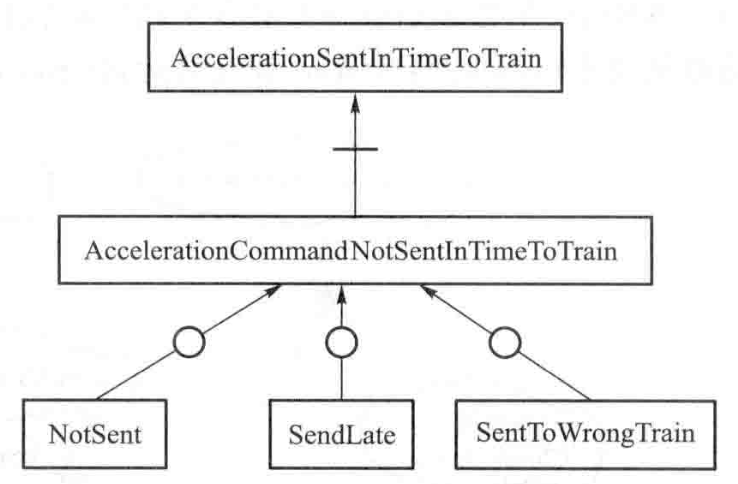
\includegraphics[width=0.45\textwidth]{img/目标模型阻碍关系示意图.png}
    \caption*{目标模型阻碍关系示意图}
\end{figure}
\vspace{-1em}

\textbf{目标之间的支持与冲突关系} \par
支持、冲突关系是对多个目标之间关系的考虑
\begin{itemize}
    \item Support链接表示一个目标对其他目标的支持作用,支持关系可以被处理为OR精化关系
    \item Conflict链接表示一个目标的实现对其他目标的实现有阻碍作用  
\end{itemize}

在二元的支持、冲突关系中,也可以使用如下标识标记关系
\begin{itemize}
    \item ++ (Make):一个目标的成功可以直接保证另一个目标的成功
    \item + (Help):一个目标的成功可以让另一个目标更容易成功
    \item $-$ (Hurt):一个目标的成功会使得另一个目标的成功更加困难
    \item $--$ (Break):一个目标的成功会直接导致另一个目标的失败
\end{itemize}

\begin{figure}[H]
	\centering
	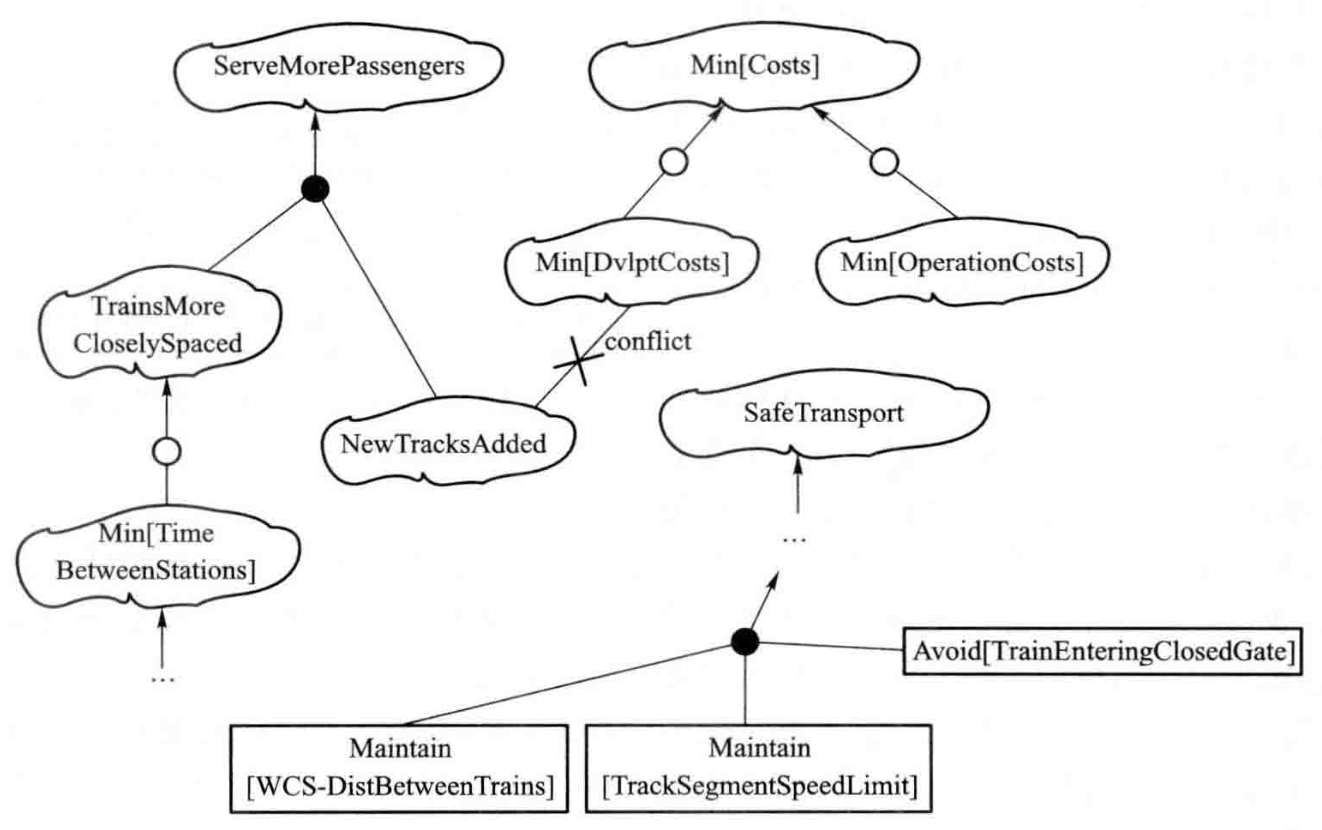
\includegraphics[width=0.7\textwidth]{img/目标模型精化关系示意图.png}
    \caption*{目标模型精化关系示意图}
\end{figure}
\vspace{-1em}

\textbf{目标与其他需求模型元素的链接} \par
目标可以与其他模型元素建立关系,这些模型元素有主体(agent)、场景(scenario)、操作(operation)、任务(task)、资源(resource)和UML元素等。

\begin{figure}[H]
	\setcounter{subfigure}{0}
	\centering
	\vspace{-1em}	
	\subfloat[目标与主体之间的关系示例]{
		\begin{minipage}[t]{0.54\linewidth}
		\centering
		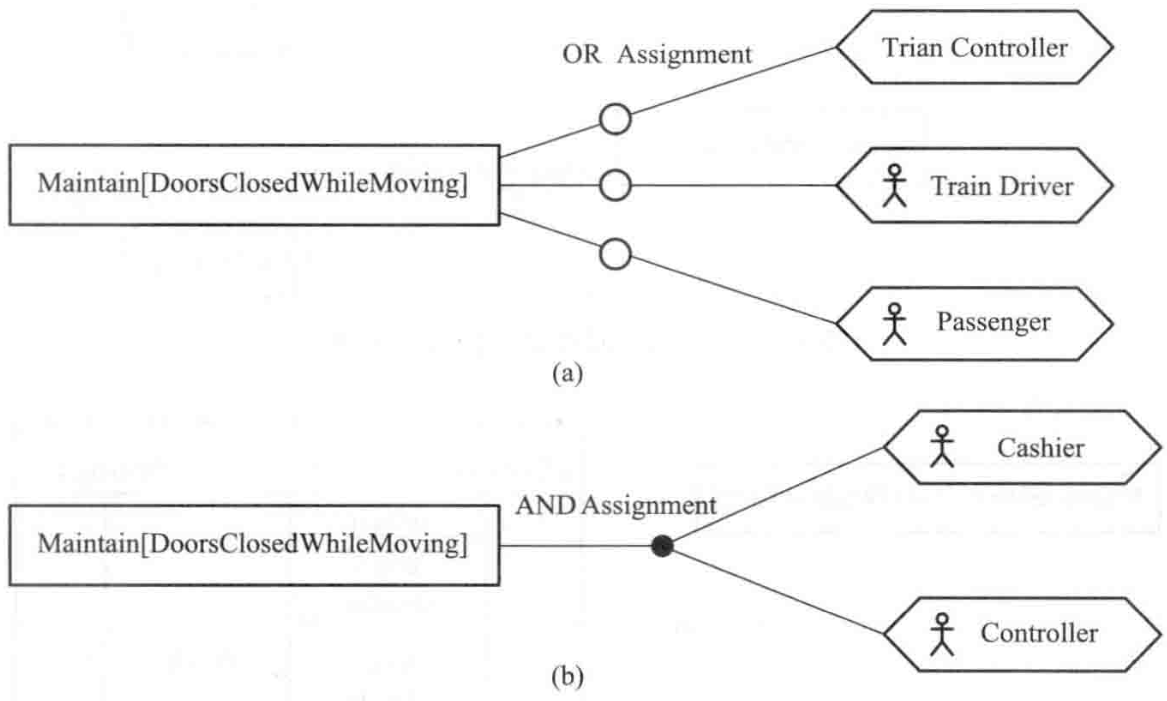
\includegraphics[width=\linewidth]{img/目标与主体之间的关系示例.png}
		\end{minipage}
	}
	\subfloat[目标与操作之间的关系示例]{
		\begin{minipage}[t]{0.43\linewidth}
		\centering
		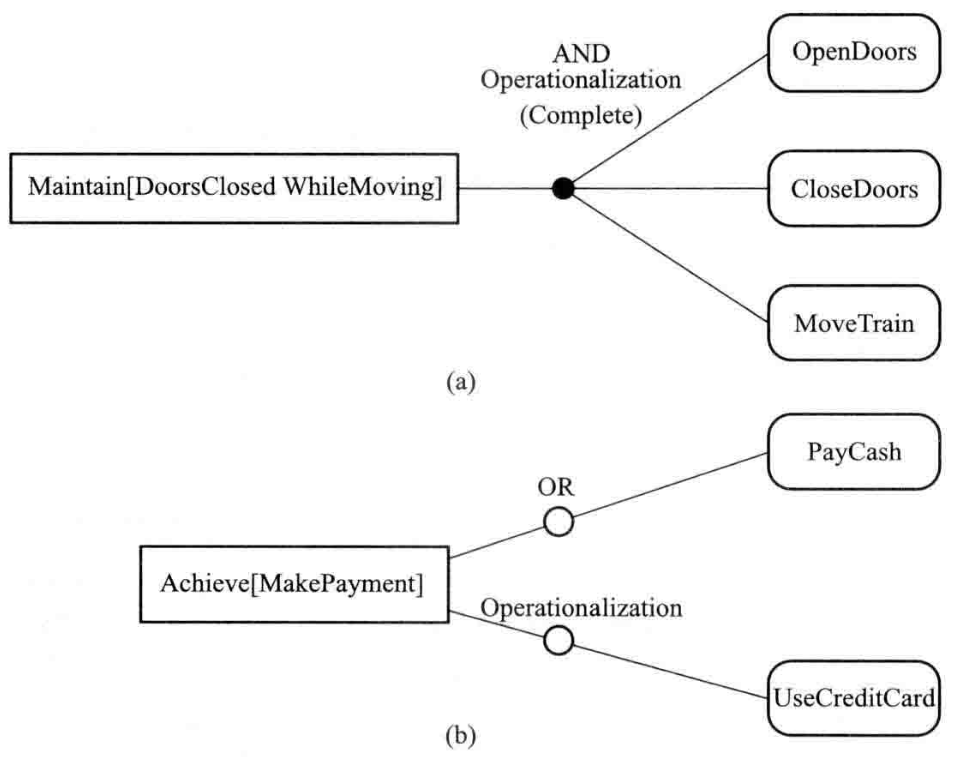
\includegraphics[width=\linewidth]{img/目标与操作之间的关系示例.png}
		\end{minipage}
	}
	\centering
	\vspace{-1em}
\end{figure}

\subsubsection{面向目标的方法}
面向目标方法的处理过程 
\begin{itemize}
    \item 高层目标的获取:现状和背景的分析(画布、评估)
    \item 低层目标的获取 :需求获取与目标分析
    \begin{itemize}
        \item 已有目标的验证和细化 (基于目标分析)
        \item 基于场景的方法等等 (基于目标实现)
    \end{itemize}
    \item 目标分析 :精化与分解
    \begin{itemize}
        \item 建立系统的目标模型 
    \end{itemize}
    \item 目标实现 
    \begin{itemize}
        \item 收集与目标相关的需求信息,讨论可能的候选解决方案,确定最终的系统详细需求和解决方案 
    \end{itemize}
\end{itemize}

\begin{figure}[H]
	\centering
	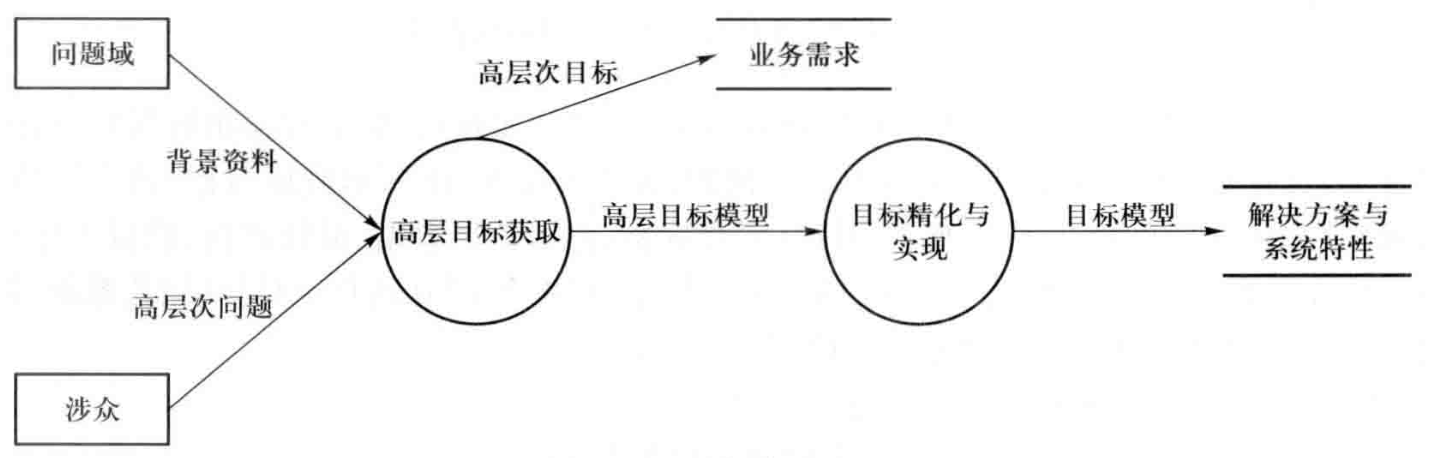
\includegraphics[width=0.85\textwidth]{img/目标分析过程.png}
\end{figure}

\paragraph{高层目标的获取}~{} \par
对于连锁商店销售系统项目,通过分析其问题P1$\sim$P4, 并建立最高层目标BR1$\sim$BR4,这些目标可以被抽取定义为业务需求并将它们组织为目标模型。

\begin{figure}[H]
	\centering
	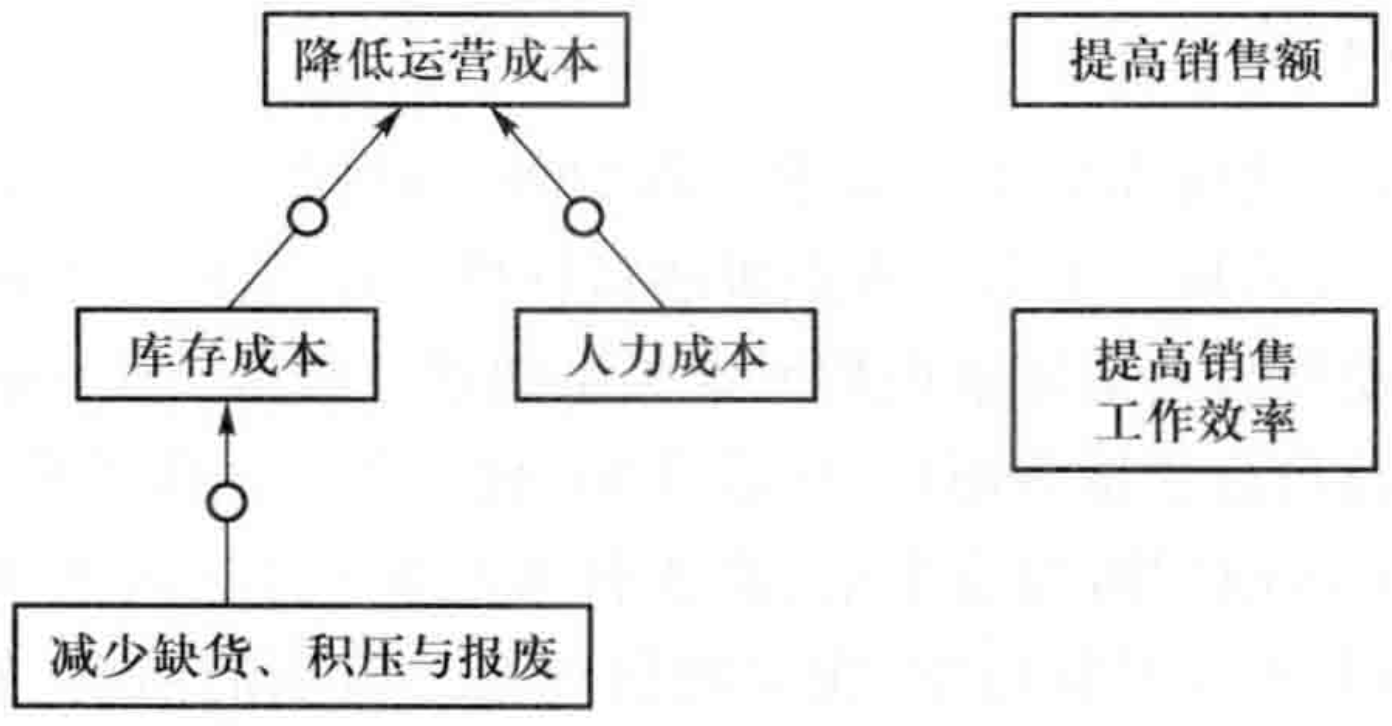
\includegraphics[width=0.48\textwidth]{img/连锁商店销售系统的高层目标模型.png}
    \caption*{连锁商店销售系统的高层目标模型}
\end{figure}
\vspace{-1em}

\paragraph{目标精化}~{} \par

\ding{172} 获取对高层目标的描述

通过收集背景资料,运用面谈、原型等需求获取方法,可以收集对高层目标的描述信息。常见的描述信息包括企业规章、政策,任务描述,业务过程和场景描述。

\ding{173} 从高层目标描述中发现AND精化关系

\begin{itemize}
    \item 同一个目标有不同场景:每个G$i$代表一个典型场景,任意G$i$与G$j$代表不同的场景;
    \item 完成目标有连续过程:每个G$i$代表G完成过程中的一个状态,G$i$、G$i+1$代表两个连续的状态;
    \item 完成目标需要有多个方面紧密配合:G$i$与G$j$紧密联系或互相支持;
    \item 目标有不同质量环境及表现:每个G$i$代表不同质量要求下的G的完成。
\end{itemize}

\ding{174} 从高层目标描述中发现“候选办法”,发现OR精化关系

\ding{175} 考虑阻碍目标(avoid目标)实现的情况

\ding{176} 发现目标冲突关系

\ding{177} 对高层目标问“How”,对低层目标同“Why”,完善层次结构

\vspace{-2em}
\begin{figure}[H]
	\centering
	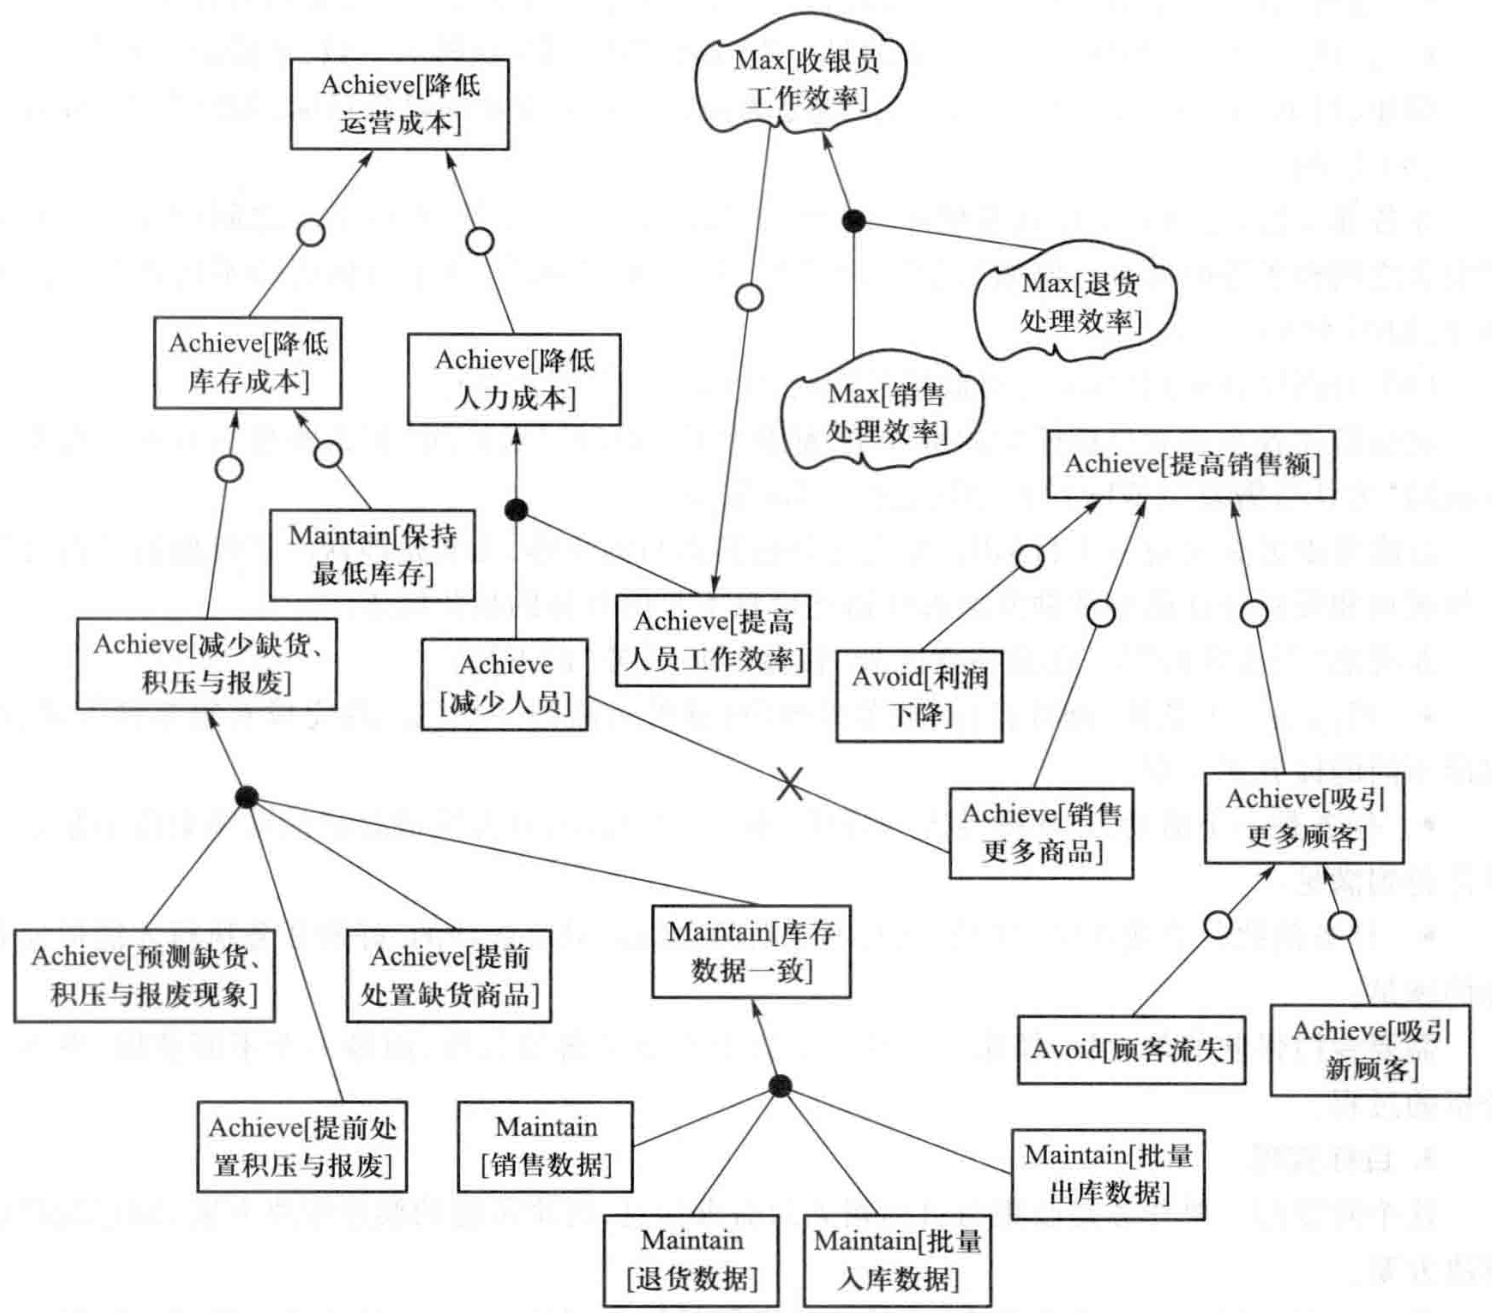
\includegraphics[width=0.88\textwidth]{img/连锁商店销售系统的完整目标模型.png}
    \caption*{\textbf{连锁商店销售系统的完整目标模型}}
\end{figure}
\vspace{-1em}

\paragraph{目标实现}~{} \par
将最底层目标分配给主体(人$+$系统)
\begin{figure}[H]
	\centering
	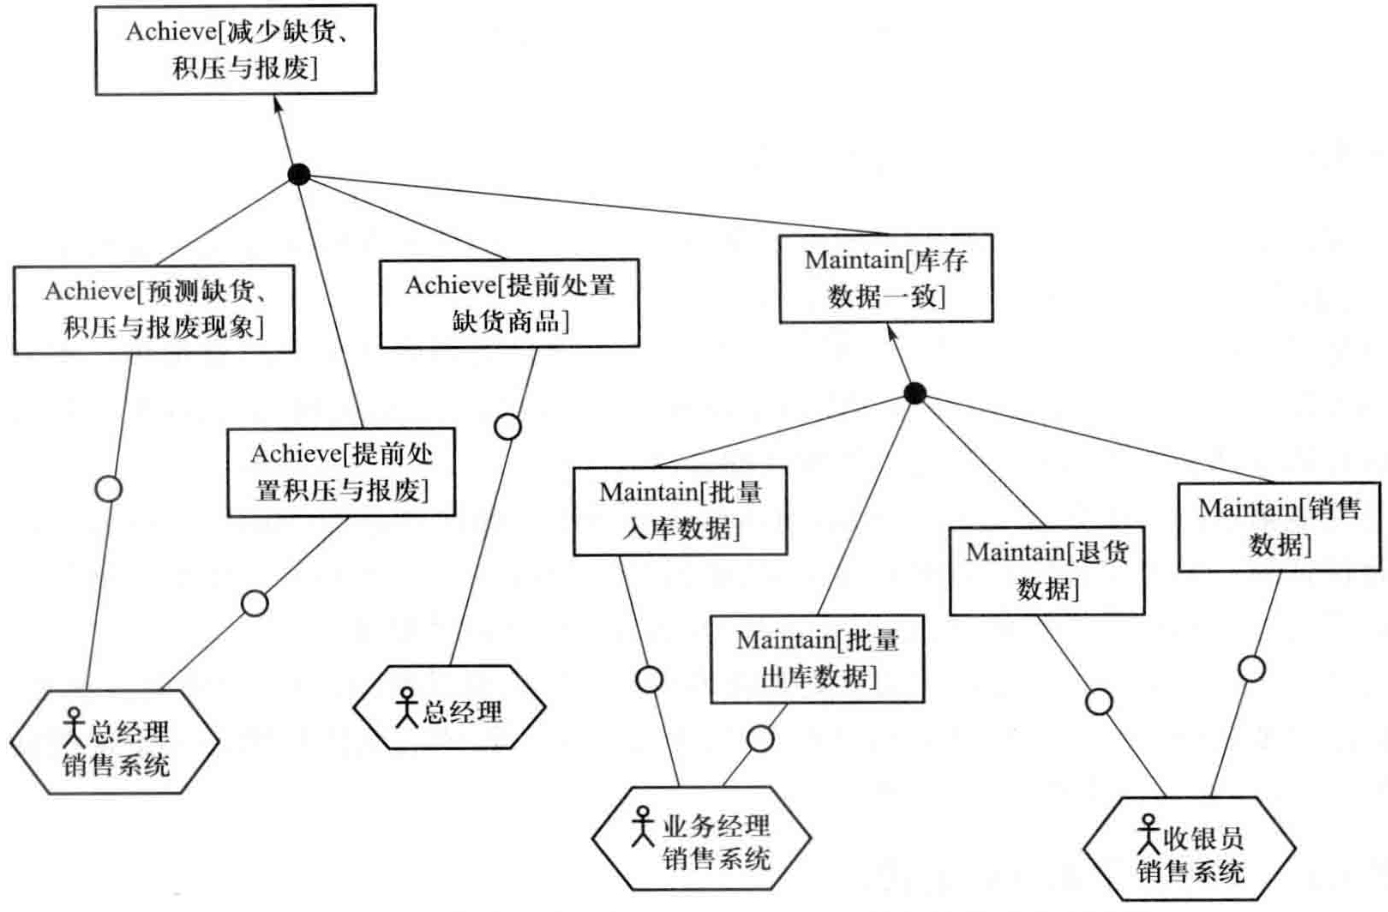
\includegraphics[width=0.75\textwidth]{img/连锁商店销售系统的目标模型片段的主体分配实现示例.png}
    \caption*{连锁商店销售系统的目标模型片段的主体分配实现示例}
\end{figure}
\vspace{-1em}

设计实现最底层目标的操作(任务:细粒度用例/场景)
\begin{figure}[H]
	\centering
	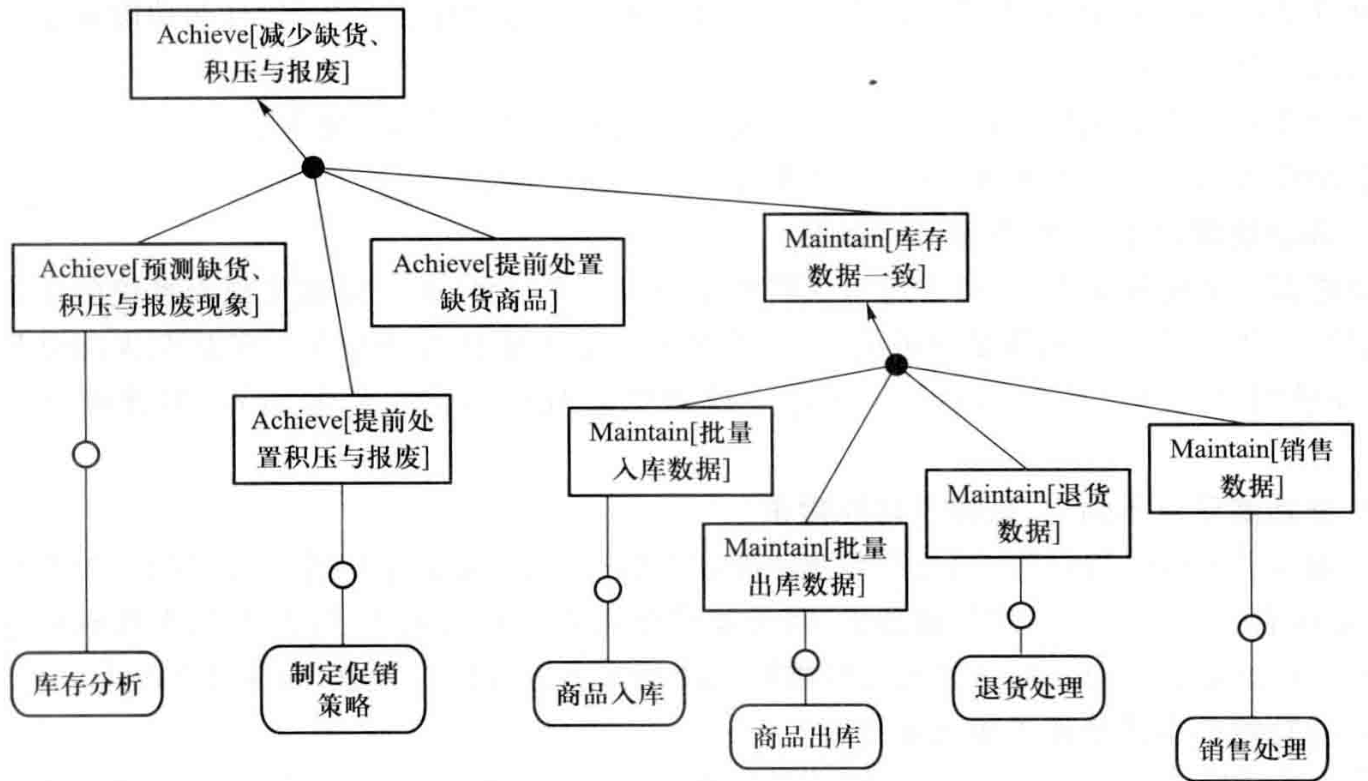
\includegraphics[width=0.85\textwidth]{img/连锁商店销售系统的目标模型片段的操作实现示例.png}
    \caption*{连锁商店销售系统的目标模型片段的操作实现示例}
\end{figure}
\vspace{-1em}
	\section{涉众分析}

\subsection{什么是涉众}
涉众是指所有能够影响软件系统的实现, 或者会被实现后的软件系统所影响的个人和团体。

涉众分析围绕一个组织的各个部门内的员工所负责的业务展开
\begin{itemize}
    \item 所有的描述和胜败条件都和业务直接相关
\end{itemize}

此类涉众分析的难度随着组织机构的复杂性和不确定性增长而增加
\begin{itemize}
    \item 部门内$\rightarrow$部门间$\rightarrow$新业务部门$\rightarrow$组织间$\rightarrow$大众用户(互联网产品)
\end{itemize}


\subsection{涉众分析的过程}
涉众分析与前景与范围的定义是交织进行的,互为依赖
\begin{figure}[H]
	\centering
	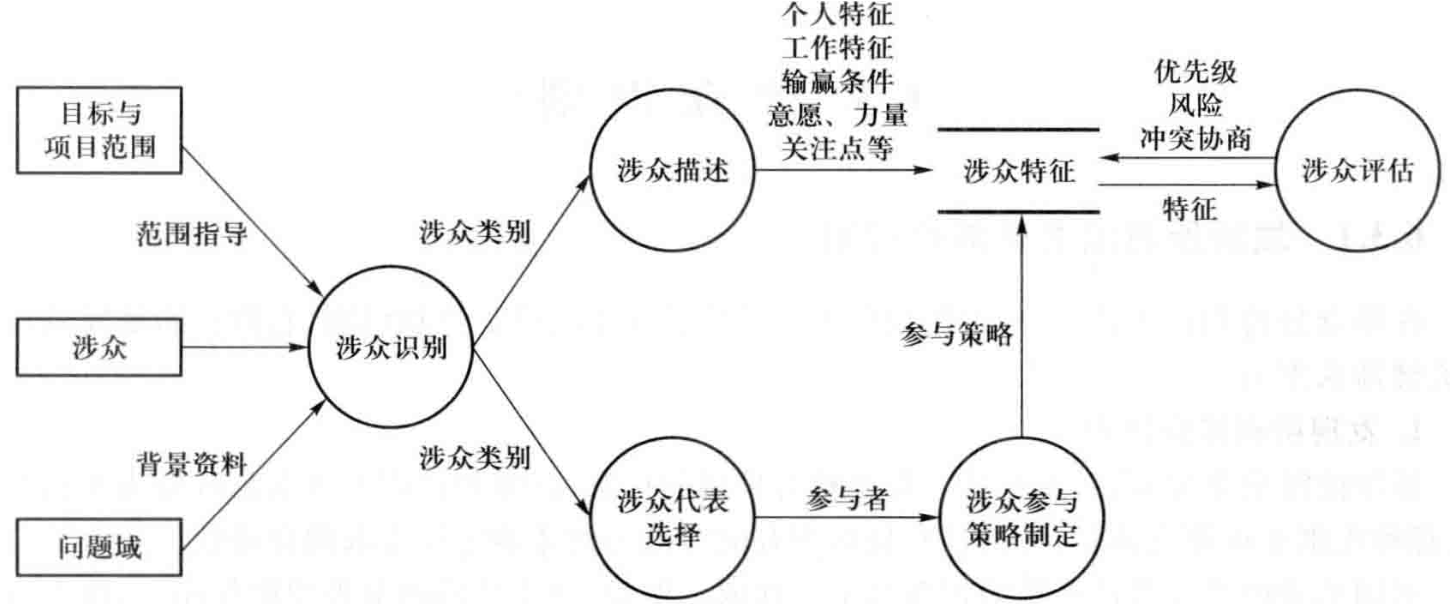
\includegraphics[width=0.85\textwidth]{img/涉众分析过程.png}
\end{figure}


\subsection{涉众识别}

\subsubsection{涉众识别的基本原则}
\begin{itemize}
    \item 涉众类别需要细分,发现所有类别
    \begin{itemize}
        \item 每一类涉众的所有成员都能够一致、稳定的从相同立场、相同视角来看待相同的软件系统
    \end{itemize}
    \item 发现比较关键的涉众
    \begin{itemize}
        \item 需要分析他们各自的赢利条件,以在相互妥协中尽力实现一个共赢的结局
    \end{itemize}
    \item 涉众群体不是固定不变的,需要持续维护
    \begin{itemize}
        \item 对涉众的理解不是一个完成之后就可以结束的活动,而是应该在完成之后继续保持适当的关注
    \end{itemize}
\end{itemize}

如果互动及其关注点属于项目的目标与范围,那么涉众就属于关键涉众
\begin{figure}[H]
	\centering
	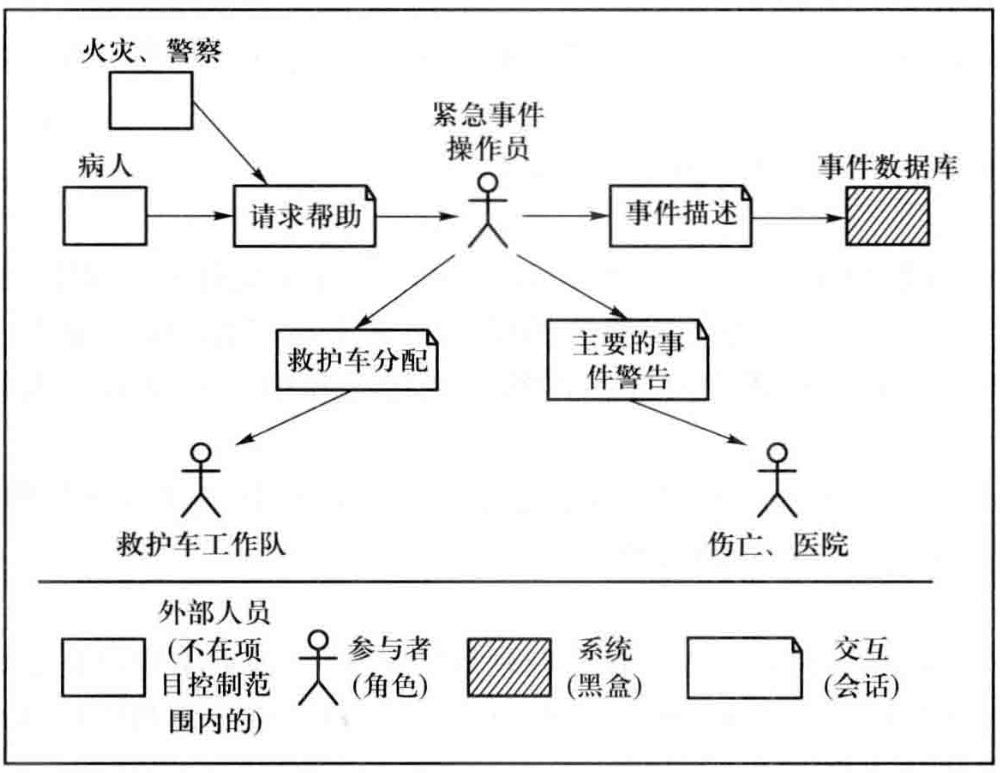
\includegraphics[width=0.65\textwidth]{img/救护车调度系统的交互网络草图.png}
    \caption*{救护车调度系统的交互网络草图}
    \vspace{-1em}
\end{figure}

\subsubsection{识别涉众的方法}
\begin{itemize}
    \item 简单方法:先膨胀后收缩方法
    \begin{itemize}
        \item 尽可能列出涉众后尝试合并,易用但可能有遗漏
    \end{itemize}
    \item 经典方法:涉众网络 方法
    \begin{itemize}
        \item 用容易发现的涉众(客户、管理者、投资人)出发
        \item 与初始涉众一起“膨胀—收缩”,集体确定关键涉众列表,再请列表中的新代表加入讨论,直到列表稳定
    \end{itemize}
    \item 经验方法:检查列表方法
    \begin{itemize}
        \item 在实践中人们总结出子常见的涉众类别列表,并据此指导涉众识别工作
    \end{itemize}
\end{itemize}

软件系统开发中常见的涉众类别有以下几种(检查列表方法)
\begin{itemize}
    \item 用户:最终使用和操作产品的人,关注软件功能 
    \item 客户:为软件系统的开发付费的人,关注经济上的成本、收益
    \item 开发者:负责实现软件系统的人,关注技术上的成本和收益
    \item 管理者:参与软件系统开发事务管理的人,投资方管理者、执行负责人、项目管理者,关注系统的开发进程
    \item 领域专家:在问题域中具有丰富知识的专家,关注软件中的知识(概括性、综合性) 
    \item 政府力量:法律法规、长远规划、政策意向等,起约束和指导作用
    \item 市场力量:组织中的市场部门人员,关注用户的想法
    \item 维护人员:系统的非功能属性,例如质量
\end{itemize}

利用\textbf{主体依赖模型}(Actor Dependency Model, ADM)分析涉众互动,识别关键涉众类别
\begin{itemize}
    \item 目标依赖(goal dependency):依赖者希望被依赖者满足一个条件,但不会规定怎样满足该条件。
    \item 软目标依赖(soft goal dependency):一种特殊类型的目标依赖,其条件是无法量化描述的。
    \item 任务依赖(task dependency):依赖者希望被依赖者执行特定任务。任务依赖比目标依赖更加具体,因为满足目标可以执行很多任务,被依赖者有自己的选择权。而任务依赖直接为被依赖者规定了任务。
    \item 资源依赖(resource dependency):依赖者希望被依赖者提供资源实体(抽象信息或者实物材料)为自己所用,但不关注提供资源需要被依赖者执行的行为和解决的问题。  
\end{itemize}
\begin{figure}[H]
	\centering
	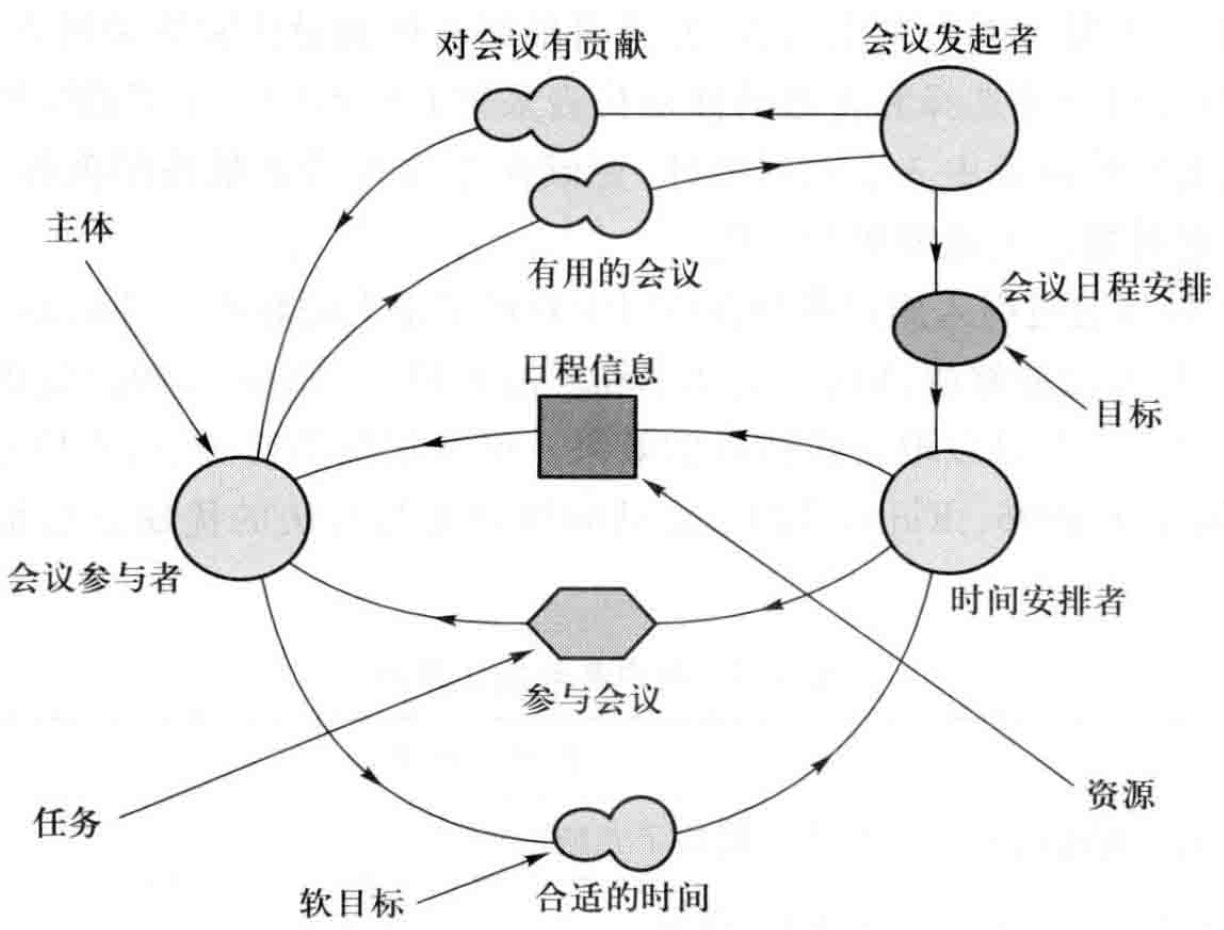
\includegraphics[width=0.7\textwidth]{img/主体依赖模型示例.png}
    \caption*{\textbf{主体依赖模型示例}}
    \vspace{-1em}
\end{figure}

\subsection{涉众描述}

\subsubsection{描述哪些内容}
\begin{itemize}
    \item L1:根据软件系统的功能前景寻找涉众
    \item L2:从涉众对象那里获取需求
    \item L3:分析涉众的输赢条件,实施共赢策略 
    \item L4:涉众对系统的影响力:了解涉众实现、监控和评估软件系统的能力,分析涉众的力量和影响范围;了解涉众实现、监控和评估软件系统的意愿,即分析涉众的关注点和兴趣取向
    \item L5:了解涉众的个人特征和工作特征,以便在涉众固定的情况下对软件系统的功能进行合理的调整  
\end{itemize}

\subsubsection{涉众简单特征描述}
涉众类别的特征描述
\begin{table}[H]
    \centering
    \begin{tabular}{|c|c|}
    \hline
    \multirow{4}{*}{个人特征}    & 年龄、性别、学历、职业、职务    \\ \cline{2-2} 
                             & 生活方式、个性、对新技术的态度   \\ \cline{2-2} 
                             & 技能                \\ \cline{2-2} 
                             & 身体能力及限制,例如色盲      \\ \hline
    \multirow{3}{*}{工作特征}    & 任务                \\ \cline{2-2} 
                             & 使用状况(利用程度、使用频率等)  \\ \cline{2-2} 
                             & 技能和经验(新手$\sim$专家) \\ \hline
    \multirow{3}{*}{地理和社会特征} & 地理:区域、国家          \\ \cline{2-2} 
                             & 文化背景              \\ \cline{2-2} 
                             & 社会关系              \\ \hline
    \end{tabular}
\end{table}

“化学制品跟踪系统”的涉众描述示例
\vspace{-0.8em}
\begin{center}
    \begin{longtable}{|Wc{3cm}|m{9cm}|}
        \hline
        涉众       & \multicolumn{1}{c|}{特征}                                                                               \\ \hline
        药剂师      & 药剂师将使用系统请求来自供应商和仓库的化学制品。药剂师每天多次使用系统,主要用于跟踪进出实验室的化学制品容器。药剂师需要在供应商目录中查找指定化学制品                                                                      \\ \hline
        采购者      & 采购者在采购部门处理其他用户所提交的化学制品请求,他们与外部的供应商建立联系,制定并发出订单。采购者对化学制品几乎不了解,因此将需要简单的查询机制来查找供应商目录。采购者不使用系统中容器跟踪这一特性。每个采购者平均每天使用系统10次                             \\ \hline
        化学制品仓库人员 & 化学制品仓库人员包括三个技师,管理着多达500 000种化学制品容器。他们将处理来自药剂师的请求并提供可用的容器,向供应商请求新的化学制品以及跟踪进出仓库的所有容器的流向,他们是货存清单和化学制品使用报告特性的唯一使用者。由于交易量大,化学制品仓库人员所使用的系统功能必须是自动化并且高效 \\ \hline
        卫生和安全人员  & 卫生和安全人员使用系统是为了生成符合官方关于化学制品使用和处理规则的季度报表。这些报表必须提前定义,并不需要特别查询能力,当官方的规则改变时,卫生和安全管理人员可能每年多次要求变化报表中的内容。报表变更优先级最高                                       \\ \hline
    \end{longtable}
\end{center}
\vspace{-3.7em}

\subsubsection{涉众深度信息描述}
\begin{itemize}
    \item 对项目的关注点和兴趣所在,态度是反对还是赞同
    \item 对项目的期望,成为项目赢家的条件
    \item 可能受到的项目的影响,影响的具体内容及影响程度
    \item 可以对项目施加的影响,力量的施加点及其强度
    \item 客户洞察中的移情图可以很好的补充涉众的深度信息  
\end{itemize}

自助餐厅在线订餐系统的涉众扩展特征描述
\vspace{-0.8em}
\begin{center}
    \begin{longtable}{|m{2cm}<{\centering}|m{2.4cm}|m{2.4cm}|m{2.4cm}|m{2.4cm}|}
    \hline
    涉众       & \multicolumn{1}{c|}{主要目标}                         & \multicolumn{1}{c|}{态度}                                             & \multicolumn{1}{c|}{主要关注点}                      & \multicolumn{1}{c|}{约束条件}                            \\ \hline
    公司管理层    & 提高员工生产率;节约自助餐厅的费用            & 强烈承诺完成版本2;如果有条件尽早完成版本3                         & 使用该系统所节约的费用必须超过开发和使用此系统的费用 & 无                               \\ \hline
    自助餐厅工作人员 & 更高效地利用了工作人员的整个工作时间;提高了客户的满意度 & 担心与工会的关系和可能的裁员,否则很愿意接受新系统                      & 保证工作                       & 培训工作人员使用Internet的技能;需要有送货的人员和车辆 \\ \hline
    顾客       & 可以更好地选择食物;节约了时间;更加方便         & 因为在自助餐厅和饭店就餐有社交作用,所以积极支持新系统,但使用系统的次数可能没有期望的次数多 & 使用要简单;送货可靠;食物选择要有效         & 需要访问公司的内部网络                     \\ \hline
\end{longtable}
\end{center}
\vspace{-3.7em}

\subsection{涉众评估}

\subsubsection{优先级评估}
\begin{itemize}
    \item (面向业务的)涉众并不是完全平等的,有些涉众比其他涉众更为重要
    \item 优先考虑涉众的基本特征,尤其是(涉众所完成的)任务特征 
\end{itemize}

一个医务(体检)软件的User/Task矩阵
\begin{table}[H]
    \centering
    \begin{tabular}{|c|c|c|c|}
    \hline
    用户群体 & 任务      & 群体数量 & 优先级 \\ \hline
    入院秘书 & 收集病人的数据 & 25   & 2   \\ \hline
    护士   & 查看体检信息  & 490  & 3   \\ \hline
    管理员  & 软件安装与维护 & 12   & 1   \\ \hline
    \end{tabular}
\end{table}


\subsubsection{风险评估}
\textbf{基于涉众特征与态度化解涉众风险策略}
\begin{itemize}
    \item 基于特征化解举例:亲子兴趣班
    \begin{itemize}
        \item 大人与小朋友一起参与:环境设定者(客户)$\rightarrow$ 参与者(用户)
        \item 良好的产品体验打造亲子品牌:被影响者(潜在用户/客户)$\rightarrow$ 参与者
    \end{itemize}
    \item 基于态度化解举例:电子竞技产业
    \begin{itemize}
        \item 与地方政府文化产业发展相结合:强反对者 $\rightarrow$ 强支持者
        \item 成功的赛事运营与未成年人游戏时长限制:弱反对者 $\rightarrow$ 弱支持者
    \end{itemize}
\end{itemize}

\begin{figure}[H]
	\centering
	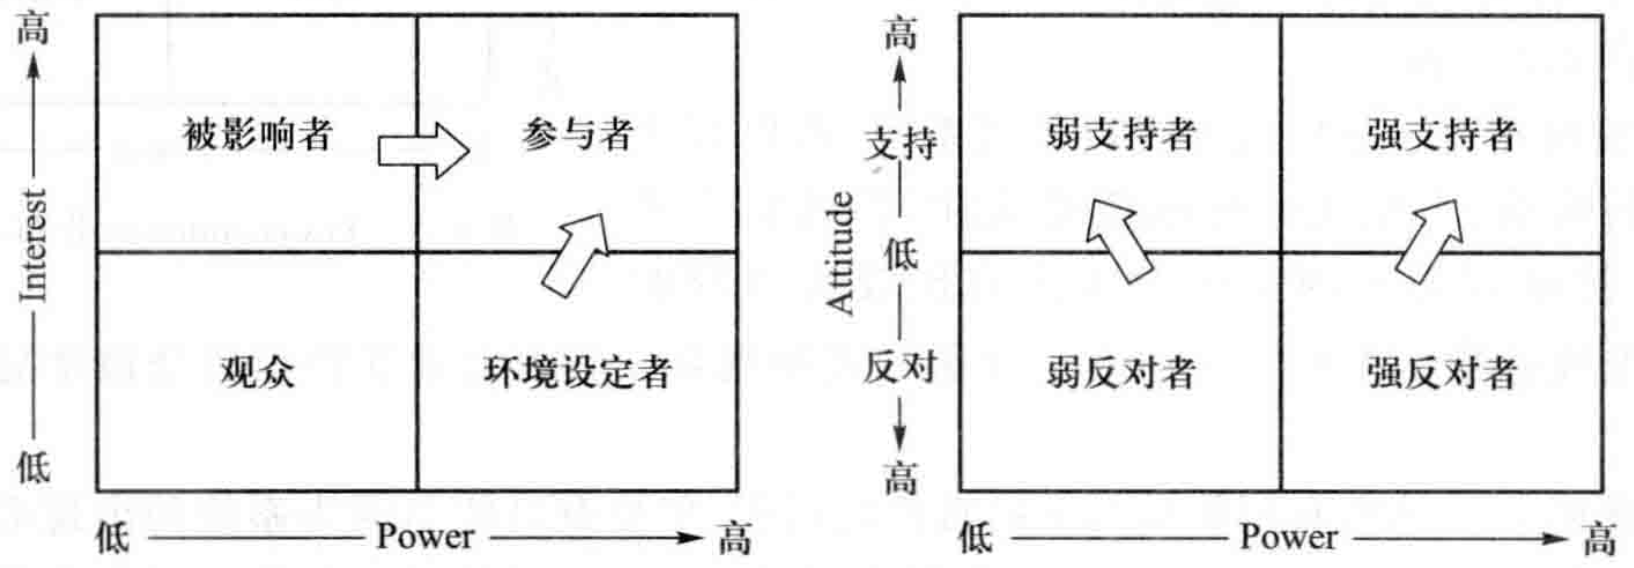
\includegraphics[width=0.8\textwidth]{img/化解涉众风险策略图.png}
    \caption*{\textbf{化解涉众风险策略图}}
    \vspace{-1em}
\end{figure}

\subsubsection{共赢分析}
\textbf{Stakeholder/Issue关系图}
\begin{itemize}
    \item 列出系统的所有涉众类别,明确描述他们的兴趣和对系统的期望
    \item 从涉众们的兴趣和期望中发现背后涉及的共同问题(Issue)
    \item 建立涉众类别和问题的关联,如果某个涉众类别对一个Issue存在兴趣,那么该涉众类别和这个Issue就存在关联关系
    \item 对每一个Stakeholder/Issue关系,标明该关系上面所被寄予的期望
\end{itemize}

\begin{figure}[H]
	\centering
	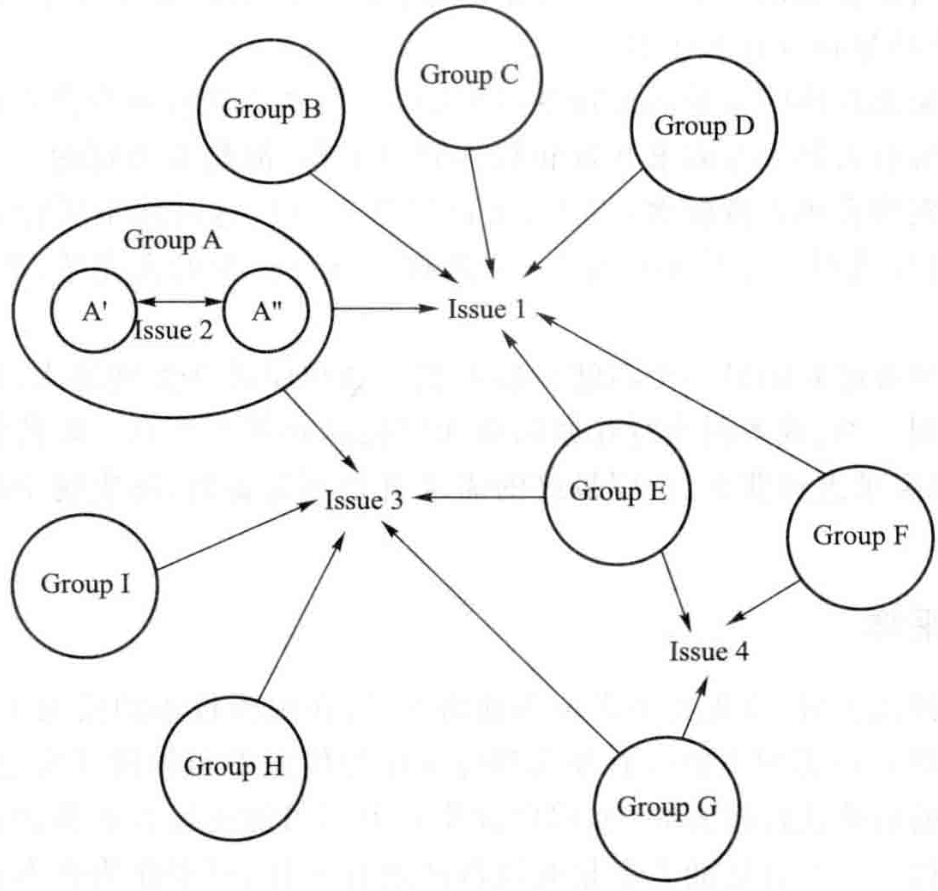
\includegraphics[width=0.5\textwidth]{img/Stakeholder-Issue关系图.png}
    \caption*{\textbf{Stakeholder/Issue关系图}}
    \vspace{-1em}
\end{figure}

基于Stakeholder/Issue关系图的共赢分析
\begin{itemize}
    \item 如果某个Stakeholder/Issue关系上所寄予的期望与项目的业务需求无法保持一致,那么它关联的涉众就在该Issue的问题上和项目整体目标存在冲突
    \begin{itemize}
        \item 涉众和项目负责人互相调整、折中 
        \item 重新评估项目的可行性 
    \end{itemize}
    \item 如果Stakeholder/Issue关系图中某个Issue所关联的不同关系标识有互相冲突的期望,那么就意味着它所关联的涉众在该Issue上存在需求冲突
    \begin{itemize}
        \item 分析各冲突方成为项目赢家的条件 
        \item 适当的调整,化解冲突 
        \item 分析项目在该Issue上的目标、约束和可选方案,并提供给冲突方进行权衡,促进他们之间协商解决   
    \end{itemize}
\end{itemize}

\subsubsection{利用目标模型深入评估涉众}
基于拥有者的目标模型,可以更好地执行涉众评估:
\begin{itemize}
    \item 将目标模型的目标配到主体
    \item 根据目标的优先级安排主体的优先级
    \item 根据目标的风险确定主体的风险
    \item 根据目标分析深入分析主体间的互动
    \begin{itemize}
        \item 根据目标冲突可以发现深层次的主体冲突
        \item 根据目标的冲突情况协商解决主体间的冲突
    \end{itemize}
\end{itemize}

\begin{figure}[H]
    \vspace{-0.5em}
	\centering
	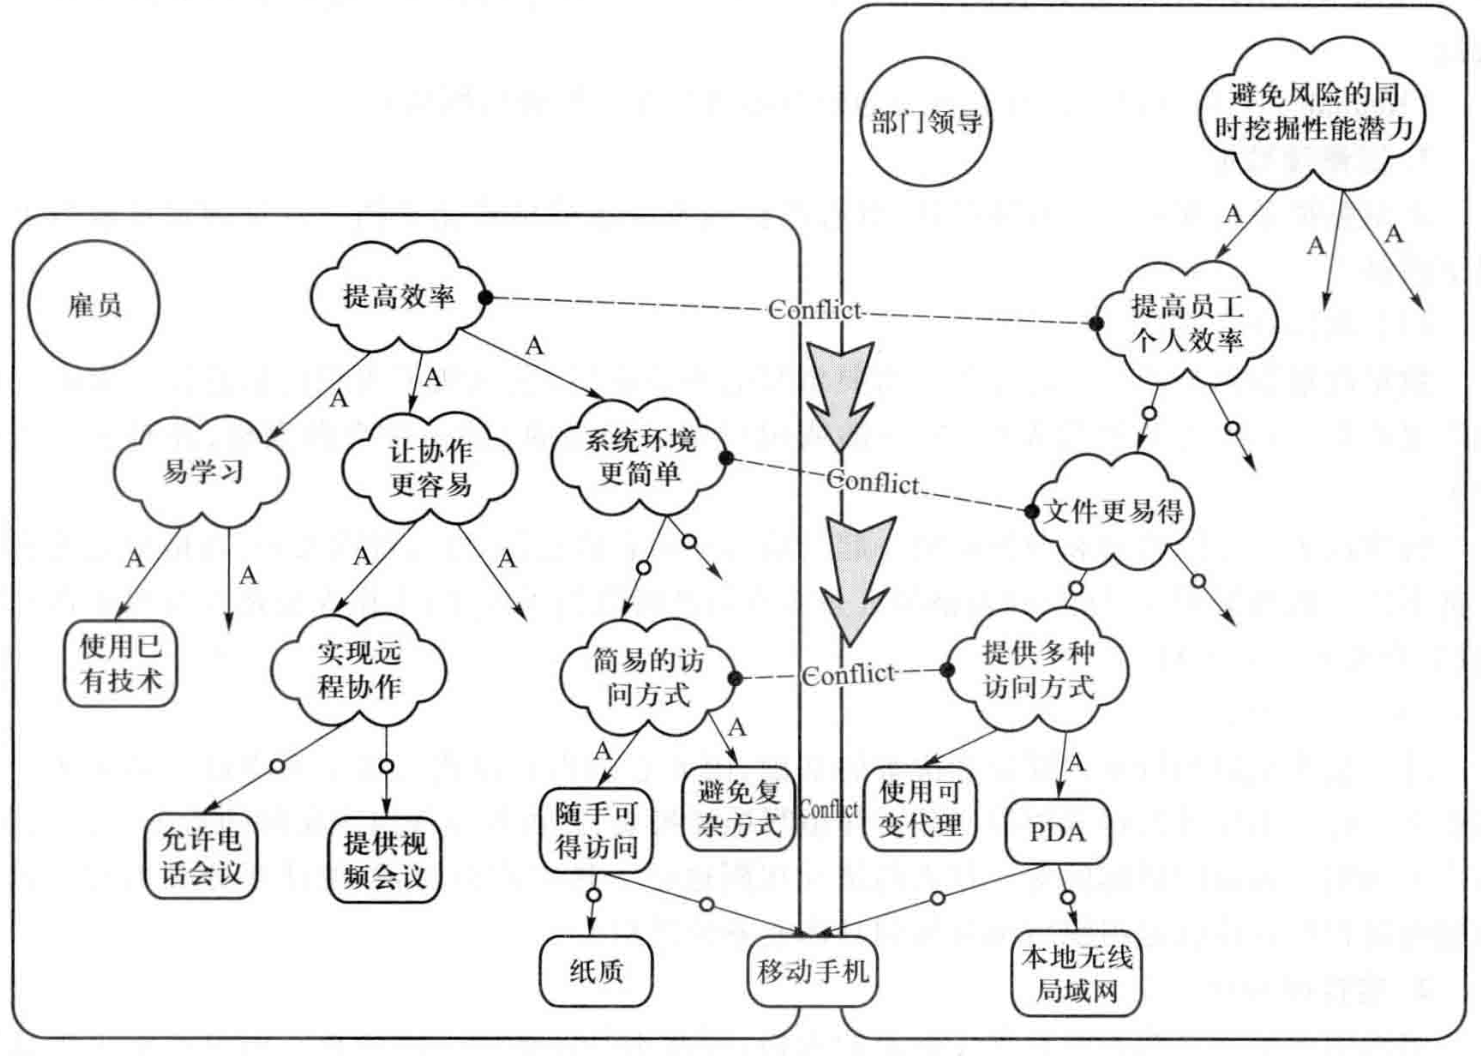
\includegraphics[width=0.68\textwidth]{img/拥有者的目标模型示例.png}
    \caption*{拥有者的目标模型示例}
    \vspace{-1.3em}
\end{figure}

\subsection{涉众代表选择}

\subsubsection{涉众采样}
\begin{itemize}
    \item 完整采样:每种涉众类别都有自己的代表
    \item 态度积极:愿意提供帮助
    \item 数量适中
    \begin{itemize}
        \item 太少:个人看法倾轧群体共同看法
        \item 太多:达成一致困难 
        \item 代表数量的准确数字要视项目的上下文环境来确定,一般为6$\sim$10
    \end{itemize}
    \item 比例恰当
    \vspace{-0.8em}
	\begin{multicols}{2}
        \begin{itemize}
            \item 计算机技能
            \item 业务技能
        \end{itemize}
	\end{multicols}
	\vspace{-1em}
\end{itemize}


\subsubsection{用户替代源}
在无法找到合适的涉众代表时,需求工程师可以考虑寻找一些涉众替代源——那些因为业务关系而和用户频繁接触的人。涉众替代源因为和用户在工作上存在频繁接触,所以能够较好地理解用户的真实想法,自然也就能够部分地代替他们发表看法。
\vspace{-0.8em}
\begin{multicols}{3}
    \begin{itemize}
        \item 市场人员
        \item 服务咨询人员
        \item 技术支持人员
        \item 领域专家
        \item (出色的)产品经理
    \end{itemize}
\end{multicols}
\vspace{-1em}

\subsection{涉众参与策略制定}

\subsubsection{制定涉众参与的基本策略}
代表们在合适的时间参与合适的工作
\begin{figure}[H]
    \vspace{-0.5em}
	\centering
	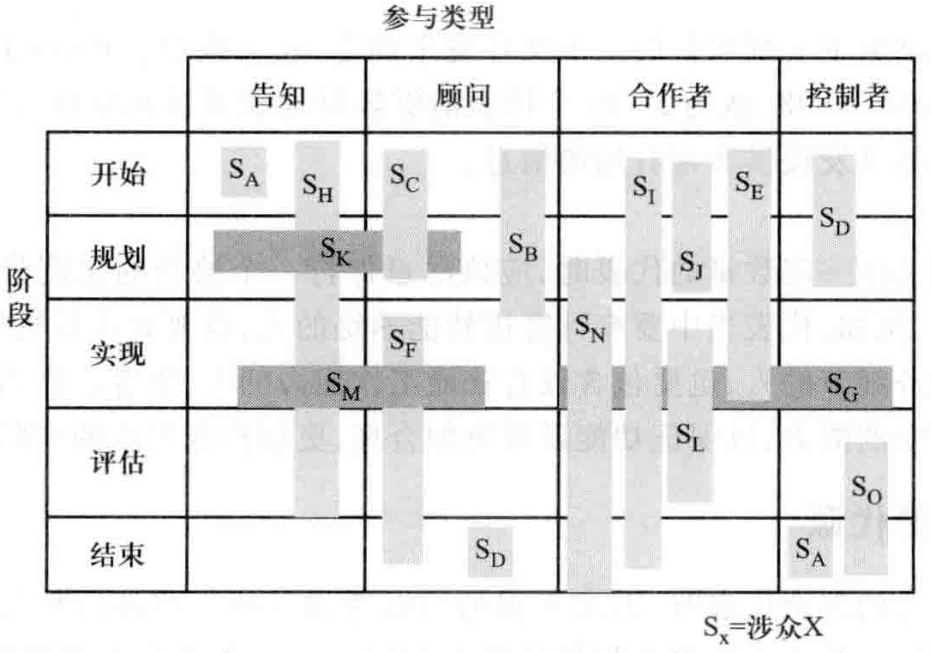
\includegraphics[width=0.6\textwidth]{img/涉众参与矩阵.png}
    \caption*{涉众参与矩阵}
    \vspace{-1em}
\end{figure}

\subsubsection{敏捷方法——用户参与}
\begin{itemize}
    \item 建立和用户的直接联系 
    \item 用户参与软件系统开发的整个过程 
    \item 反馈设计:最终的软件系统和用户的活动行为密切相关
    \item 主要通过社区来实现
\end{itemize}

用户参与的优缺点
\begin{table}[H]
    \centering
    \begin{tabular}{|c|l|}
    \hline
    \multirow{5}{*}{优点} & 会有更精确的用户需求,进而提高了系统的质量                                                             \\ \cline{2-2} 
                        & 可以避免发生代价昂贵的系统故障                                                                   \\ \cline{2-2} 
                        & 能提高用户对系统的接受度                                                                      \\ \cline{2-2} 
                        & 用户能够更有效的理解和使用系统                                                                   \\ \cline{2-2} 
                        & 可以提高组织内决策制定过程的参与度                                                                 \\ \hline
    \multirow{4}{*}{缺点} & 采集和管理巨量原始数据会花费很多时间                                                                \\ \cline{2-2} 
                        & 需要解决直接接触用户和对设计施加影响的困难                                                             \\ \cline{2-2} 
                        & \begin{tabular}[c]{@{}l@{}}用户通常不愿意在别人的观察下工作,而且研究\\ 发现用户在被观察时并不是真的在工作\end{tabular} \\ \cline{2-2} 
                        & 难以安排对用户工作过程的观察                                                                    \\ \hline
    \end{tabular}
\end{table}
	\section{基于用例/场景模型展开用户需求获取}

\subsection{用户需求的组织}
\begin{itemize}
    \item 场景/用例模型驱动
    \begin{itemize}
        \item 整理和归类需求获取行为得到的信息(框架)
        \item 指导和组织需求获取行为的开展
        \item 为详细信息的分析提供背景基础和上下文知识 
    \end{itemize}
    \item 承上启下
    \vspace{-0.8em}
	\begin{multicols}{2}
    \begin{itemize}
        \item 展开上一层(业务需求)
        \item 准备下一层的展开(系统级需求)
    \end{itemize}
	\end{multicols}
\end{itemize}

\subsection{场景}
\begin{itemize}
    \item $[$Zorman 1995]将场景定义为对系统和环境行为的局部描述
    \item $[$Plihon 1998]将场景定义为对行为或者事件序列的描述,序列中的行为和事件是系统需要完成的一个任务的特殊示例。
    \item $[$Jarke 1996]认为场景包含有行为序列和行为发生的环境,环境描述了行为的主体、客体和上下文设置
    \item 以上的描述都不足以作为场景的准确定义,人们也很难给场景下一个非常准确的定义[Rolland 1998a]
    场景强调系统同外部环境互动以完成预期任务
\end{itemize}

\subsection{场景与用例在需求工程中的定位}
\begin{itemize}
    \item 场景
    \begin{itemize}
        \item 具有重点描述真实世界的特征,利用情景、行为者之间的交互、事件随时间的演化等方式来叙述性的描述系统的使用
    \end{itemize}
    \item 用例
    \begin{itemize}
        \item 相关场景集合的叙述性的文本描述 
        \item 最早在Objectory方法[Jacobson 1992]中提出的
    \end{itemize}
    \item UML将用例定义为“在系统(或者子系统或者类)和外部对象的交互当中所执行的行为序列的描述,包括各种不同的序列和错误的序列,它们能够联合提供一种有价值的服务”[Rumbaugh 2004]。
    \item 商业模式中的场景一般需要多个用例来支撑(商业模式设计:讲故事$\rightarrow$场景)
\end{itemize}



	\section{面谈}

\subsection{概述}
\begin{itemize}
    \item 面对面的会见(face-to-face meeting)被认为是最具丰富内容的交流方法
    \item 实践当中应用最为广泛的需求获取方法之一 
    \item 可以获得的信息内容包括 
    \vspace{-0.8em}
	\begin{multicols}{2}
    \begin{itemize}
        \item 事实和问题 
        \item 被会见者的观点 
        \item 被会见者的感受 
        \item 组织和个人的目标 
    \end{itemize}
	\end{multicols}
\end{itemize}

\begin{figure}[H]
	\centering
	
\includegraphics[width=0.6\textwidth]{img/面谈的基本过程.png}
    \caption*{面谈的基本过程}
    \vspace{-1em}
\end{figure}

\subsection{准备面谈}

\subsubsection{准备工作}
面谈淮备的主要工作包括以下几方面
\vspace{-0.8em}
\begin{multicols}{2}
    \begin{itemize}
        \item 阅读背景资料 
        \item 确定面谈主题和目标 
        \item 选择被会见者 
        \item 通知被会见者:电话或邮件等正式的途径 
        \item 确定问题和类型   
    \end{itemize}
\end{multicols}
\vspace{-1em}

\subsubsection{问题类型}
准备问题不仅仅是要清楚面谈的内容,更要清楚提问题的方法,尤其是要恰当地使用各种不同问题类型
\vspace{-0.8em}
\begin{multicols}{4}
    \begin{itemize}
        \item 开放式问题
        \item 封闭式问题
        \item 程序性提示 
        \item 探究式问题
        \item 诱导式问题
        \item 元问题
        \item ……
    \end{itemize}
\end{multicols}
\vspace{-1em}

问题基本上可以分为两种类型:开放式问题和封闭式问题

\textbf{开放式问题} \par
被会见者对答复的选择可以是开放和不受限制的,他们可能答复两个词,也可能答复两段话

在希望得到丰富(具有一定深度和广度)信息时,开放式问题比较合适

开放式问题举例
\vspace{-0.25em}
{\kaishu \begin{compactitem}
    \item “你觉得把所有的经理都置于一个内联网内怎么样?”
    \item “请解释你是如何做进度决策的?”
    \item “对公司中企业对企业电子商务的当前状态有何看法?”
\end{compactitem}}

开放式问题的优点
\begin{itemize}
    \item 让被会见者感到自在;
    \item 会见者可以收集被会见者使用的词汇,这能反应他的教育、价值标准、态度和信念;
    \item 提供丰富的细节;
    \item 对没采用的进一步的提问有启迪作用;
    \item 让被会见者更感兴趣;
    \item 容许更多的自发性;
    \item 会见者可以在没有太多准备的情况下进行面谈。
\end{itemize}

开放式问题的缺点
\begin{itemize}
    \item 提此类问题可能会产生太多不相干的细节;
    \item 面谈可能失控;
    \item 开放式的回答会花费大量的时间才能获得有用的信息量;
    \item 可能会使会见者看上去没有准备。
\end{itemize}

\textbf{封闭式问题} \par
答案有基本的形式,被会见者的回答是受到限制的 

封闭式问题举例
\vspace{-0.25em}
{\kaishu \begin{compactitem}
    \item “项目存储库每个星期更新多少次?”
    \item “电话中心一个月平均收到多少个电话?”
    \item “下列信息中哪个对你最有用:(1)填好的客户投诉单;(2)访问web站点的客户的电子邮件投诉;(3)与客户面对面的交流;(4)退回的货物。”
    \item “列出头两项需要优先考虑的改善技术基础设施的事项。”
\end{compactitem}}

封闭式问题的优点
\vspace{-0.8em}
\begin{multicols}{2}
    \begin{itemize}
        \item 节省时间
        \item 切中要点
        \item 保持对面谈的控制
        \item 快速探讨大范围问题
        \item 得到贴切的数据
    \end{itemize}
\end{multicols}
\vspace{-1em}

封闭式问题的缺点
\vspace{-0.8em}
\begin{multicols}{2}
    \begin{itemize}
        \item 使得被会见者厌烦
        \item 得不到丰富的细节
        \item 出于上述原因,失去主要思想
        \item 不能建立和面谈者的友好关系
    \end{itemize}
\end{multicols}
\vspace{-1em}

\textbf{程序性提示} \par
程序性提示是针对一些人的思维特点而设计的面谈问题[Pitts 2007],它们的使用是程序性的,也就是说到了特点的面谈程序点,就应该使用相应的程序性提示问题。

\begin{table}[H]
    \centering
    \begin{tabular}{|c|l|}
    \hline
    提示                         & \multicolumn{1}{c|}{示例}                                                           \\ \hline
    \multirow{3}{*}{总结和反馈}     & 你能不能总结一下系统的功能?                                                                    \\ \cline{2-2} 
                               & 你能不能总结一下一个成功系统的必备特征?                                                              \\ \cline{2-2} 
                               & 在使用的时候,你希望能够从系统当中得到什么类型的信息反馈?                                                     \\ \hline
    \multirow{3}{*}{重复和改述}     & 能不能再说一次系统的哪些特征是重要的?                                                               \\ \cline{2-2} 
                               & 你能不能详细的重新叙述一下使用系统的步骤?                                                             \\ \cline{2-2} 
                               & 在使用系统的时候你会做出什么决定?                                                                 \\ \hline
    \multirow{3}{*}{建立场景和细节描述} & 有什么是你现在能做,却在新系统中不能做的?                                                             \\ \cline{2-2} 
                               & 在什么情况下,功能是必需的?                                                                    \\ \cline{2-2} 
                               & \begin{tabular}[c]{@{}l@{}}设想现在是6个月之后,你需要评估系统的成功状况,你会使用哪\\ 些标准来做出评价?\end{tabular} \\ \hline
    \multirow{3}{*}{抗辩}        & 你能不能想出什么不使用系统的理由?                                                                 \\ \cline{2-2} 
                               & 你为什么会不想使用系统呢?                                                                     \\ \cline{2-2} 
                               & 你能不能想出将来可能导致系统失败或故障的原因?                                                           \\ \hline
    \end{tabular}
\end{table}
\vspace{-0.5em}

\textbf{其他重要的问题类型} \par
\begin{itemize}
    \item 探究式问题
    \vspace{-0.25em}
    {\kaishu \begin{compactitem}
    \item 为什么?
    \item 你能举个例子吗?
    \item 你能详细描述一下吗?
    \end{compactitem}}
    \item 诱导性问题
    \vspace{-0.25em}
    {\kaishu \begin{compactitem}
    \item “你和其他经理一样,都同意把财产管理计算机化,是吗” 
    \end{compactitem}}
    \item 双筒问题
    \vspace{-0.25em}
    {\kaishu \begin{compactitem}
    \item “每天你通常会做什么决策,你是怎样做的” 
    \end{compactitem}}
    \item 元问题
    \vspace{-0.25em}
    {\kaishu \begin{compactitem}
    \item 我的问题看起来相关吗?
    \item 你的回答正式吗?
    \item 你是回答这些问题的最佳人选吗?
    \item 我问了太多的问题吗?
    \item 我还应该见什么人? 
    \end{compactitem}}
\end{itemize}


\subsubsection{问题准备}
\vspace{-0.8em}
\begin{multicols}{2}
\columnseprule=0.8pt
需求工程前期
\begin{itemize}
    \item 开放式问题为主
    \item 决策层与专家为主
    \item 遵循问题$\rightarrow$目标$\rightarrow$解决方案路线
    \begin{itemize}
        \item 问题、目标
        \item 目标、任务(流程$\rightarrow$任务)
    \end{itemize}
    \item 分析基本的涉众特点
    \begin{itemize}
        \item 角色、任务、个人目标、频率、优先级
    \end{itemize}
\end{itemize}

需求工程后期
\begin{itemize}
    \item 封闭式问题为主
    \item 抓住主题与线索,例如,任务分解、流程图、界面示意等
    \item 问题针对性
    \begin{itemize}
        \item 任务分解关系
        \item 流程正确性、异常
        \item 界面中的行为、数据项
    \end{itemize}
    \item 事先准备面谈记录材料
\end{itemize}
\end{multicols}
\vspace{-1em}

面谈的问题准备示例一

{\kaishu
(面谈对象:投资人、管理者)
\vspace{-0.25em}
\begin{compactenum}[1.]
    \item 目前的业务主要碰到了哪些问题?\\
    (预计:销售效率低;积压、缺货、报废现象严重;成本较高;竞争力不足)
    \item 希望新系统能够帮助达成哪些目标?\\
    (预计:提高销售效率;减少积压、缺货、报废现象;降低成本;提高竞争力;提升销售额)\\
    (如果存在销售效率问题)
    \item 销售工作是怎样进行的?
    \item 哪些人会参与销售过程?
    \item 哪些人的哪些工作是最为瓶颈的?
\end{compactenum}
\vspace{-0.5em}
……}

面谈的问题准备示例二

{\kaishu
(面谈对象:投资人、管理者)
\vspace{-0.25em}
\begin{compactenum}[1.]
    \item 销售人员的主要工作是什么?\\
    (预计:销售处理、退货处理)
    \item 销售处理的主要过程是怎样的?
    \item 销售处理工作目前的困难有哪些?
    \item 销售处理的频率怎么样?
    \item 平均多长时间完成一次销售处理?
\end{compactenum}
\vspace{-0.5em}
……}

面谈的问题准备示例三
\vspace{-0.8em}
{\kaishu
\begin{multicols}{2}
    用例/场景描述
    \vspace{-0.25em}
    \begin{compactenum}[1.]
        \item 收银员输入会员编号;
        \item 系统显示会员信息;
        \item 收银员输入商品;
        \item 系统显示输入商品的信息;
        \item 系统显示所有已输入商品的信息;
    \end{compactenum}
    \vspace{-0.65em}
    收银员重复3$\sim$5步,直至完成所有输入
    \vspace{-0.6em}
    \begin{compactenum}[1.]
        \setcounter{enumi}{5}
        \item 收银员结束商品输入;
        \item 系统显示总价和赠品信息;
        \item 收银员请求顾客付款;
        \item 顾客支付,收银员输入支付数额;
        \item 系统显示应找零数额,收银员找零;
        \item 收银员结束销售;
        \item 系统更新数据,并打印收据。
    \end{compactenum}

    问题:
    \vspace{-0.25em}
    \begin{compactenum}[1.]
        \item 会员编号的格式是怎样的?
        \item 需要显示的会员信息有哪些?
        \item 商品是怎样输入的?
        \item 需要显示的商品信息有哪些?
        \item 系统应该怎样显示已输入商品的信息?
        \\
        \item 总价是怎样计算的?
        \item 需要显示的赠品信息有哪些?
        \item 收据的格式是怎样的?
        \item 有可能不输入会员编号吗?
        \item 有可能不输入商品吗?
        \item 有可能不结束销售吗?
        \item 付款时有其他非现金方式吗?
    \end{compactenum}   
\end{multicols}
\vspace{-1em}}

\subsubsection{面谈背后的要点:取得“共情”与“目标”的平衡}
共情
\vspace{-0.8em}
\begin{multicols}{2}
    \begin{itemize}
        \item 取得信任
        \item 激发主动性
        \item 获得更全面的问题域背景(主观)和业务意向(个人)
        \item 客户洞察:功能$\rightarrow$认知$\rightarrow$情感;面谈可视作“反向的客户洞察”
    \end{itemize}
\end{multicols}
\vspace{-1em}

目标
\vspace{-0.8em}
\begin{multicols}{2}
    \begin{itemize}
        \item 充分、正确地获取用户需求
        \item 在项目前景和范围指导下充分获取用户需求与问题域知识
        \item 利用开放式问题、探究式问题和程序性提示增强覆盖范围
        \item 利用封闭式问题确认细节
        \item 主动控制面谈过程
    \end{itemize}
\end{multicols}
\vspace{-1em}


\subsection{主持面谈}
在面谈之前的注意事项
\vspace{-0.8em}
\begin{multicols}{2}
    \begin{itemize}
        \item 记得和被会见者联系并确认面谈的安排
        \item 着装正式
        \item 不要迟到
        \item 表现出来你已经准备好参加面谈了
    \end{itemize}
\end{multicols}
\vspace{-1em}

实际的面谈分为3个阶段:开始、主体和结束
\begin{itemize}
    \item 开始:建立一个理想的氛围和环境来促进会见者和被会见者之间的交流和沟通 
    \item 主体:通过提问和倾听来完成和被会见者的信息交流,按照计划控制面谈的进行,并在必要时进行适当的调整 
    \item 结束:表示感谢并回答被会见者提出的问题。保持与被会见者的亲善和信任关系 
\end{itemize}

\subsubsection{面谈开始阶段}
面谈开始阶段需要注意的事项包括:
\vspace{-0.8em}
\begin{multicols}{2}
    \begin{itemize}
        \item 开场仪式:握手
        \item 简要重申面谈的目标
        \item 准备好笔记本、录音机或者其他记录设备
        \item 用一些一般的、轻松的、开放式的问题为开始
    \end{itemize}
\end{multicols}
\vspace{-1em}

\subsubsection{面谈主体阶段}
面谈主体阶段的注意事项包括以下几方面:
\begin{itemize}
    \item 保持有礼貌的倾听:遵循交流模式
    \item 控制面谈过程:主动打破交流模式
    \item 保持面谈主题:以面谈问题为主线索
    \item 使用探究式问题 
    \item 观察被会见者:在一个人的全部感觉中,只有7\%是通过口头(语言)交流的,38\%是通过语调交流的,55\%是通过面部表情和肢体语言交流的
    \item 使用道具支持
\end{itemize}

\subsubsection{面谈结束阶段}
面谈结束阶段的注意事项主要有以下几方面:
\begin{itemize}
    \item 面谈应该在45分钟到1小时内结束,并非要在提出所有关心的问题后才能结束面谈,相反,结束面谈应该比开始面谈更自然;
    \item 总结谈话的要点,如果有记录笔记的话可以请被会见者进行快速的检查,确保记录下了面谈的所有重要信息;
    \item 感谢被会见者,并且给时间让他们询问一些他们自己关心的问题;
    \item 握手话别。 
\end{itemize}

\subsubsection{处理面谈结果}
\vspace{-0.8em}
\begin{multicols}{2}
    \begin{itemize}
        \item 复查面谈记录:整理内容要点,进行分类 
        \item 总结面谈信息:评估面谈中所得到的信息 
        \item 完成面谈报告
    \end{itemize}
\end{multicols}
\vspace{-1em}

\subsection{面谈的类型}
\begin{itemize}
    \item 结构化面谈
    \begin{itemize}
        \item 完全按照事先的问题和结构来控制面谈 
    \end{itemize}
    \item 半结构化面谈
    \begin{itemize}
        \item 事先需要根据面谈内容准备面谈的问题和面谈结构,但在面谈过程当中,会见者可以根据实际情况采取一些灵活的策略
    \end{itemize}
    \item 非结构化面谈 
    \begin{itemize}
        \item 没有事先预定的议程安排,常见情况
        \item 甚至会在没有太多事前准备的情况下就直接到访被会见者的工作地,就某个主题开展会谈
        \item 会见者和被会见者谈话的主题可能非常广泛,而且每个主题都不会非常深入
        \item 也可能在非结构面谈中仅就某个特殊的主题进行深入的讨论
        \item 考验对领域的理解、面谈技巧、整理笔录等诸多能力
    \end{itemize}
\end{itemize}

\subsection{面谈的优点和局限性}
面谈的优点有:
\begin{itemize}
    \item 面谈的开展条件较为简单,经济成本较低;
    \item 能获得包括事实、问题、被会见者观点、被会见者态度和被会见者信仰等各种信息类型在内的广泛内容;
    \item 通过面谈,需求工程师可以和涉众(尤其是用户)建立相互之间的友好关系;
    \item 通过参与面谈,被会见者会产生一种主动为项目做出贡献的感觉,提高涉众的项目参与热情。  
\end{itemize}

面谈的缺点和局限性包括:
\begin{itemize}
    \item 面谈比较耗时,时间成本较高;
    \item 在被会见者地理分散的情况下往往难以实现面谈;
    \item 面谈参与者的记忆和交流能力对结果影响较大,尤其是面谈的成功较高的依赖于需求工程师的人际交流能力;
    \item 交谈当中常见的概念结构不同、模糊化表述、默认知识、潜在知识和态度偏见等各种问题在面谈中都不可避免,进而影响面谈的效果,导致产生不充分的、不相关的或者错误的数据;
    \item 在会见者不了解被会见者认知结构的情况下,面谈不可能取得令人满意的效果。
\end{itemize}

\subsection{和面谈相关的其他需求获取方法}

\subsubsection{群体面谈}
群体面谈的方法是将所有的涉众方集中起来,选择一个合适的地点,集中一段时间,召开一个多方共同参与的会议,一起进行需求的讨论、分析和获取。

群体面谈的需求获取方法
\vspace{-0.8em}
\begin{multicols}{2}
    \begin{itemize}
        \item 联合应用程序设计JAD
        \item 需求专题讨论会
        \item 需求中心小组
        \item 联合需求规划JRP
    \end{itemize}
\end{multicols}
\vspace{-1em}

群体面谈的优点:节约时间,有着更低的时间成本。

群体面谈的缺点:主持群体面谈比主持一对一面谈要困难的多。

群体面谈的三个阶段:计划面谈、主持面谈和分析结果
\begin{itemize}
    \item 计划面谈
    \begin{itemize}
        \item 确定参与人员:涉众、主持人、负责人、分析人员、记录人员、观察员
        \item 安排会谈时间:全职的2$\sim$4天参与会议,拟定一份议程
        \item 选择会谈地点:充足的空间,道具支持,良好的餐饮服务
        \item 准备会谈内容:面谈的主题和范围,会议的议程,需求的预期和会谈的目标,各种材料
    \end{itemize}
    \item 主持面谈
    \begin{itemize}
        \item 建立基本规则
        \vspace{-1em}
        \begin{multicols}{2}
        \begin{itemize}
            \item 按时开始和结束会议
            \item 中途休息(例如午餐)后要尽快进入状态
            \item 一次只讨论一个主题
            \item 期望每个人都为会议做出自己的贡献
            \item 要关注于问题,不要有人身批评和攻击
            \item 限制发言时间,不要个人把持会议   
        \end{itemize}
        \end{multicols}
        \vspace{-1em}
        \item 保持会议的气氛
        \item 确保每个人都积极地参与讨论
        \item 控制会议的主题
    \end{itemize}
    \item 分析结果
\end{itemize}

\subsubsection{调查问卷}
面谈方法以口头语言为主要的交流媒介,而调查问卷以文档为主要的交流媒介

适用调查问卷的情况
\begin{itemize}
    \item 系统的涉众在地理上是分布的;
    \item 系统的涉众数量众多,而且了解所有涉众的统计倾向是非常重要的;
    \item 需要进行一项探索性的研究,并希望在确定具体方向之前了解当前的总体状况;
    \item 为后续的面谈标识问题和主题,建立一个开展工作的基础框架。
\end{itemize}

调查问卷也是面谈
\vspace{-0.8em}
\begin{multicols}{2}
\begin{itemize}
    \item 适用于面谈的基本要求
    \item 留意内容导向
    \item 基于选择题的开放式问题与基于主观题的封闭式问题
\end{itemize}
\end{multicols}
\vspace{-1em}

\subsubsection{头脑风暴}
它的目的不是发现需求,而是“发明”需求,或者说是发现“潜在”需求

它鼓励参与者在无约束的环境下进行某些问题的自由思考和自由讨论,以产生新的想法 

适用情况
\vspace{-0.8em}
\begin{multicols}{2}
\begin{itemize}
    \item 发明并描述以前不存在的全新的业务功能
    \item 明确模糊的业务
    \item 在信息不充分的情况做出决策
\end{itemize}
\end{multicols}
\vspace{-1em}

头脑风暴通常包括两个阶段:想法产生阶段和想法精简阶段
\begin{itemize}
    \item 想法产生阶段
    \begin{itemize}
        \item 目的是产生出尽可能多的新的想法 
        \item 基本规则
        \begin{itemize}
            \item 充分发挥想像力,不要有任何的羁绊
            \item 产生尽可能多的想法,想法重在数量而不是质量,不要顾及想法是否荒诞
            \item 自由讨论,目的是产生新的想法,不要争吵和批评
            \item 在自由讨论当中,可以转换和组合所有已提出的想法,以产生新的想法 
        \end{itemize}
        \item 通常持续1个小时左右,特殊情况下持续$2\sim 3$个小时
    \end{itemize}
    \item 想法精减阶段
    \begin{itemize}
        \item 第一步是去除那些不值得进一步讨论的想法
        \item 第二步是把类似的意见进行归类
        \item 第三步是主持人遍历每一个未被删除的想法,确保所有参与者都对其有共同的理解
        \item 利用投票或类似方法,评估现有想法的优先级
        \item 最后,根据评估的数据,从中筛选出符合一定标准的想法作为头脑风暴方法的成果 
    \end{itemize}
\end{itemize}



	\section{原型}

\subsection{原型及原型法概述}

\subsubsection{什么是原型}
“原型是一个系统,它内化了一个更迟系统的本质特征。原型系统通常被构造为不完整的系统,以在将来进行改进、补充或者替代。” 

如果在最终的物件产生之前,一个中间物件被用来在一定广度和深度范围内表现这个最终物件,那么这个中间物件就被认为是最终物件在该广度和深度上的原型。 

包括书面描绘、场景叙述、情节串联图板、幻灯演示、动画模拟、屏幕快照和程序代码等在内的各种被用来探索和论证软件系统功能的物件都是软件的原型。

\subsubsection{为什么要使用原型}
\begin{itemize}
    \item 不确定性
    \begin{itemize}
        \item 因为对未来知识有限,而无法确定某种决策的结果
    \end{itemize}
    \item 不确定性是广泛存在的
    \begin{itemize}
        \item 科学的目的是限定、解释不确定性,不是将不确定性转换为确定性
        \item 人们厌恶不确定性:不确定性意味着不完全可控
    \end{itemize}
    \item 软件工程中存在着大量的不确定性,原型、迭代和(方法)验证是人们解决不确定性的主要手段
    \begin{itemize}
        \item 需求的不确定性:需求原型、迭代需求、需求分析技术
        \item 设计的不确定性(设计约束与设计决策):设计原型(体系结构原型)、迭代设计、设计技术
        \item 构造的不确定性(编译错误与运行表现):算法原型、调试、程序语言
        \item 测试的不确定性(缺陷分布):测试环境、测试技术
        \item 管理的不确定性(时间、成本、风险……):管理技术
        \item ……
    \end{itemize}
\end{itemize}

帮助需求工程师及早解决需求的不确定性:
\begin{itemize}
    \item 产品的用户对相关类别的产品没有经验,产品的细节需求存在着不确定性
    \item 用户在完成工作的方式上仍然存在障碍,产品在整体方案的可行性上存在着不确定性
    \item 用户在清晰说明他们的需求方面存在困难,这些相关的需求是有着不确定性的需求
    \item 需求工程师在理解用户的需求上存在困难,在澄清和理解之前,这些需求存在着不确定性
    \item 需求的可行性值得怀疑,即具体需求的可满足性存在着不确定性
    \item 创新性产品,它们的基本需求是潜在的,有着很大的不确定性
\end{itemize}


\subsection{使用原型法进行需求获取}

\subsubsection{基本过程}

\begin{figure}[H]
	\centering
    \vspace{-1em}
	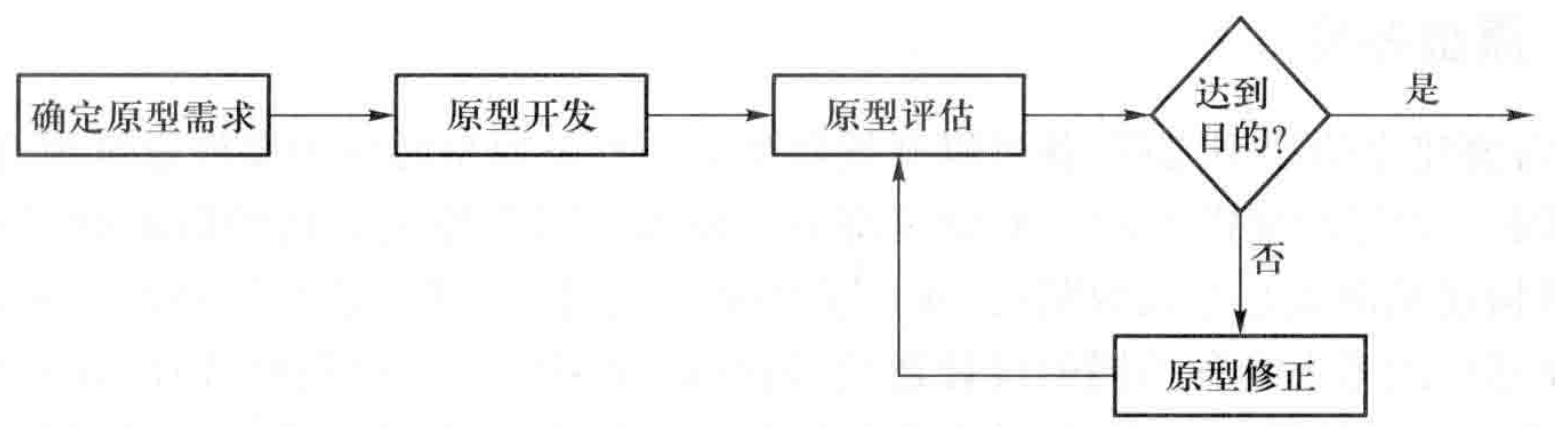
\includegraphics[width=0.65\textwidth]{img/使用原型方法获取需求的典型过程.png}
    \vspace{-1em}
\end{figure}

\subsubsection{确定原型需求}
界定不确定性
\vspace{-0.8em}
\begin{multicols}{3}
    \begin{itemize}
        \item 可能发生的需求变更
        \item 存在冲突的地方
        \item 信息不充分的地方
    \end{itemize}
\end{multicols}
\vspace{-1em}

明确不确定的维度:外观、角色和实现
\begin{itemize}
    \item 外观是指用户对原型物件的具体感觉体验,即用户在使用原型物件时会看到什么、听到什么和感觉到什么 
    \item 角色是指原型物件在用户工作中的价值,也就是说它为什么是对用户有用的
    \begin{itemize}
        \item 原型物件到底能够帮助用户完成什么样的工作
    \end{itemize}
    \item 实现是指原型物件完成功能的细节技术和方法 
\end{itemize}

\subsubsection{原型开发}
开发原型时的主要注意事项有以下几点
\vspace{-0.8em}
\begin{multicols}{2}
    \begin{itemize}
        \item 将探索不确定功能需求的原型构建得易修改
        \item 让探索可行性的原型收集充分的数据
        \item 控制开发成本
    \end{itemize}
\end{multicols}
\vspace{-1em}

\subsubsection{原型评估}
\begin{itemize}
    \item 需要获取的评估者反馈
    \vspace{-0.8em}
    \begin{multicols}{3}
    \begin{itemize}
        \item 评估者反应
        \item 评估者建议
        \item 创新思想
    \end{itemize}
    \end{multicols}
    \vspace{-1em}
    \item 可以创建一些脚本来指导评估者的体验活动 
    \item 务必要让合适的人从恰当的角度来评估原型
    \item 观察评估人员使用原型的过程
    \item 创造一个无偏见的环境,让评估人员畅所欲言
\end{itemize}

\subsubsection{原型修正}
原型修正一方面要依据评估人员的反馈, 另一方面也要考虑事先的原型调整计划。原型一定要开发的容易修改。


\subsection{抛弃式原型与演化式原型}
按照[Floyd 1984]的分类,可以将原型开发方法分为3种类型
\begin{itemize}
    \item 探索式(exploratory)
    \begin{itemize}
        \item 以缺陷需求开始继而不断调整和修正需求的原型开发方式称为探索式,要尽可能的调整各种设计选项
        \item 演示原型,严格意义上的原型
    \end{itemize}
    \item 实验式(experimental)
    \begin{itemize}
        \item 以清晰的用户需求和模糊的实现方法、实现效果、可行性开始,明确需求的可行性和技术实现方案
        \item 定义一个对原型的评估方法,确定评估的属性
        \item 试验原型
    \end{itemize}
    \item 演化式(evolutionary)
    \begin{itemize}
        \item 以清晰的原型化需求和项目积累下来的原型资产为开始
        \item 原型化的需求,也有项目积累下来的原型资产 
        \item 引示系统原型
    \end{itemize}
\end{itemize}

% 设定尺寸单位
\setlength{\TPHorizModule}{\textwidth}
\setlength{\TPVertModule}{\textwidth}
 
% 排版文本框
\begin{textblock}{0.5}(0.775,1.35)
{\fangsong
\begin{compactitem}
    \item 演示原型
    \begin{compactitem}
        \item 主要被用在启动项目阶段 
        \item 目的让用户相信应用系统的开发是可行的 
    \end{compactitem}
    \item 严格意义上的原型
    \begin{compactitem}
        \item 主要被用在分析需求阶段 
        \item 用来阐明用户界面或者系统功能的某些特定方面 
    \end{compactitem}
    \item 试验原型
    \begin{compactitem}
        \item 主要被用在构建系统阶段 
        \item 帮助开发者澄清他们所面对的一些和系统构建相关的技术问题 
    \end{compactitem}
    \item  引示系统原型
    \begin{compactitem}
        \item 会被开发在系统开发的各个阶段 
        \item 用作最终系统的构建核心 
    \end{compactitem}
\end{compactitem}}
\end{textblock}

  
探索式和实验式方法产生的原型产品又被称为抛弃式原型 
\begin{itemize}
    \item 花费最小的代价,争取最快的速度 
    \item 可能会使用简易的开发工具和不成熟的构造技术 
    \item 可能会忽略或简化处理原型目的不相关的功能特征 
    \item 要\textbf{坚决抛弃抛弃式原型}
\end{itemize}

演化式原型方法产生的原型产品被称为演化式原型
\begin{itemize}
    \item 质量要从一开始就能达到最终系统的要求 
    \item 要易于进行扩展和频繁改进,因此开发者必须重视演化式原型的设计 
    \item 仅应该被用于处理清晰的需求、规格说明和技术方案 
\end{itemize}

\subsection{控制原型开发成本}

\subsubsection{依据抛弃式特征控制原型成本}
因为基于不确定的需求基础,所以抛弃式原型难免反复修改,导致代码质量较低,应该坚决抛弃。

抛弃式原型的贡献不在于它的代码,而是它所包含的内容,它说明了正确的需求和正确的技术方案,如果认识不到这一点,他们就只能得到低质量的代码,而丢失真正宝贵的内容。

控制抛弃式原型的成本
\begin{itemize}
    \item “不要过于详细地构建抛弃式原型,只要它能够满足原型制作的目标就足够了。要抵制住诱惑,也要顶住用户的压力,不要向抛弃式原型添加更多的功能。”[Wiegers2003]
\end{itemize}

\subsubsection{控制水平原型的开发成本}
\vspace{-0.8em}
\begin{multicols}{2}
    \begin{itemize}
        \item 水平原型方法
        \begin{itemize}
            \item 它仅仅实现选定功能所有层次中的某些特定层次 
            \item 建立的原型产品称为水平原型
            \item 要把注意力集中在概括性需求和工作流问题上 
        \end{itemize}
        \item 垂直原型方法
        \begin{itemize}
            \item 它会触及到选定功能实现的所有层次
            \item 建立的原型产品称为垂直原型
            \item 要保证真实实现它的各种功能
        \end{itemize}
        \item 用尽可能低的成本开发水平原型
    \end{itemize}
\end{multicols}
\vspace{-1em}

\subsubsection{用尽量简单的介质降低成本}
\begin{figure}[H]
	\centering
    \vspace{-1em}
	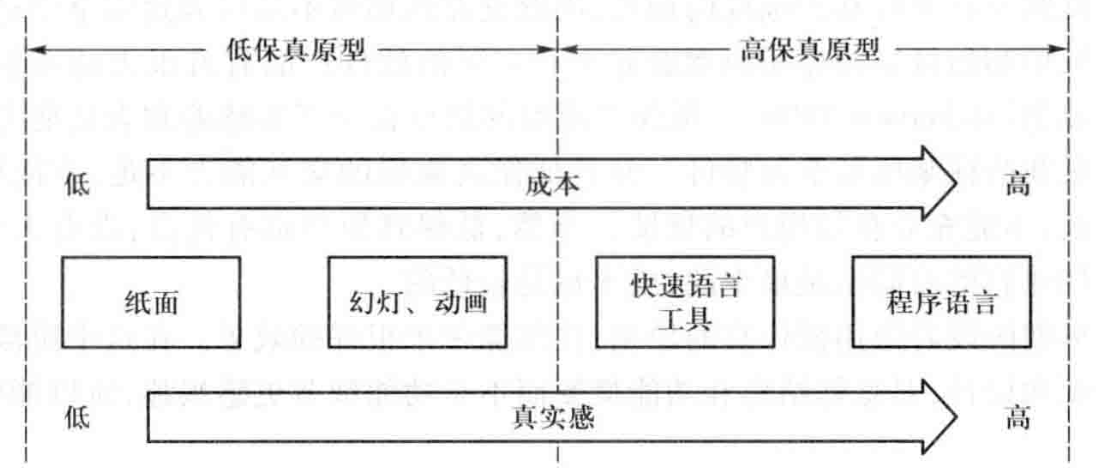
\includegraphics[width=0.65\textwidth]{img/原型的常见介质.png}
    \caption*{原型的常见介质}
    \vspace{-1em}
\end{figure}

\subsection{善用故事板原型}
\begin{figure}[H]
	\centering
    \vspace{-1em}
	
\includegraphics[width=0.6\textwidth]{img/故事板原型.png}
    \vspace{-1em}
\end{figure}

故事板最早是好莱坞在设计电影场景和卡通故事时使用的,卡通制作者通过勾画出一系列相连的图片来展示一个卡通故事,具有更直观、可视化的故事叙述能力

将原来分散的功能与步骤组织成故事,让普通人能够更好地体验与评估

原型和用例/场景通常结合使用[Mannio 2001]:为需要探索和澄清的用例/场景建立故事板原型,或者依据故事板原型的评估结果建立清晰、明确的用例/场景描述

\begin{figure}[H]
	\centering
    \vspace{-1em}
	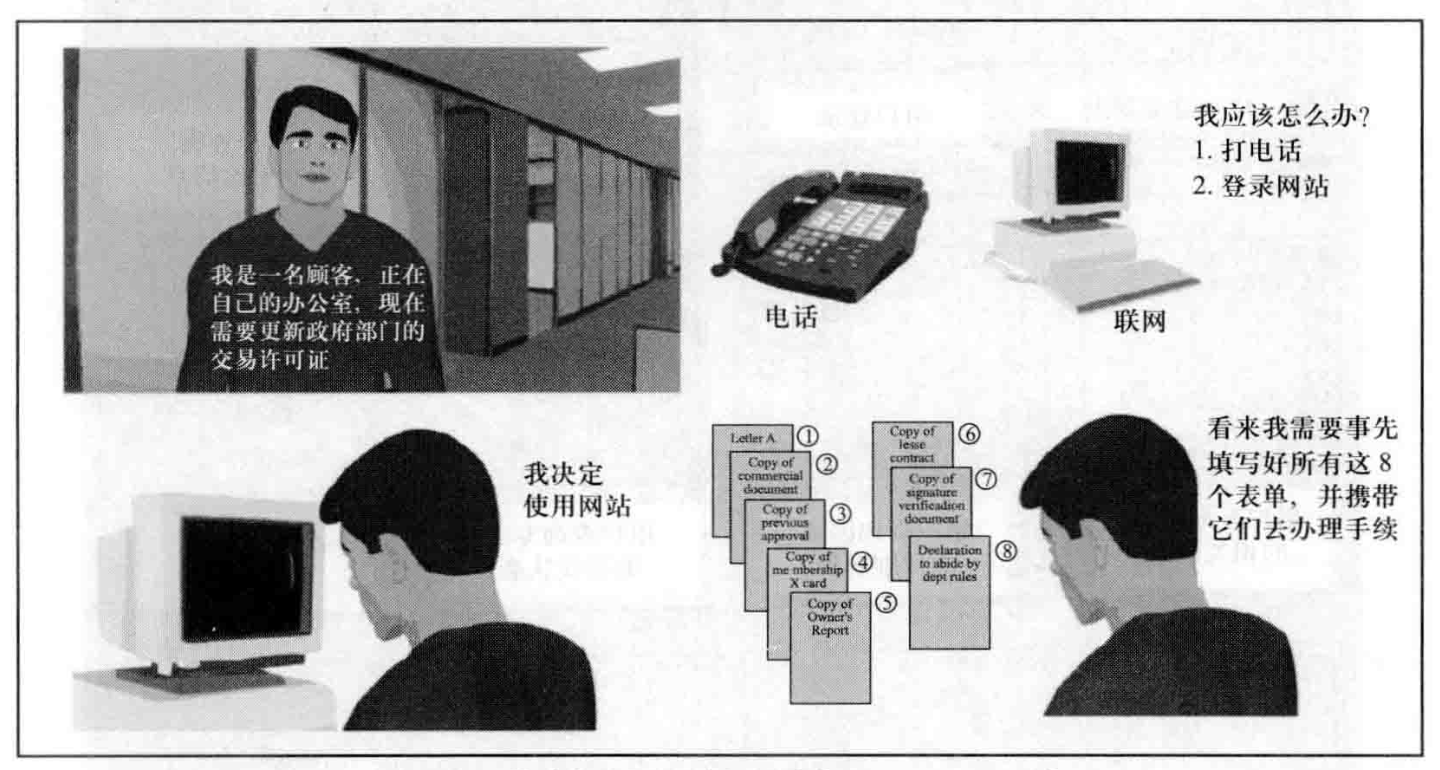
\includegraphics[width=0.75\textwidth]{img/故事板原型示例.png}
    \caption*{故事板原型示例}
    \vspace{-1em}
\end{figure}

故事板原型构建
\begin{itemize}
    \item 明确故事板原型要素
    \vspace{-0.8em}
    \begin{multicols}{3}
    \begin{itemize}
        \item 角色(Who)
        \item 内容(What)
        \item 方法(How)
    \end{itemize}
    \end{multicols}
    \vspace{-1em}
    \item 建不同类型的故事板原型
    \begin{itemize}
        \item 被动(Passive)故事板原型$\rightarrow$连环画
        \item 主动(Active)故事板原型$\rightarrow$漫画
        \item 交互(Interactive)故事板原型$\rightarrow$网页   
    \end{itemize}
\end{itemize}

\begin{figure}[H]
	\centering
    \vspace{-0.5em}
	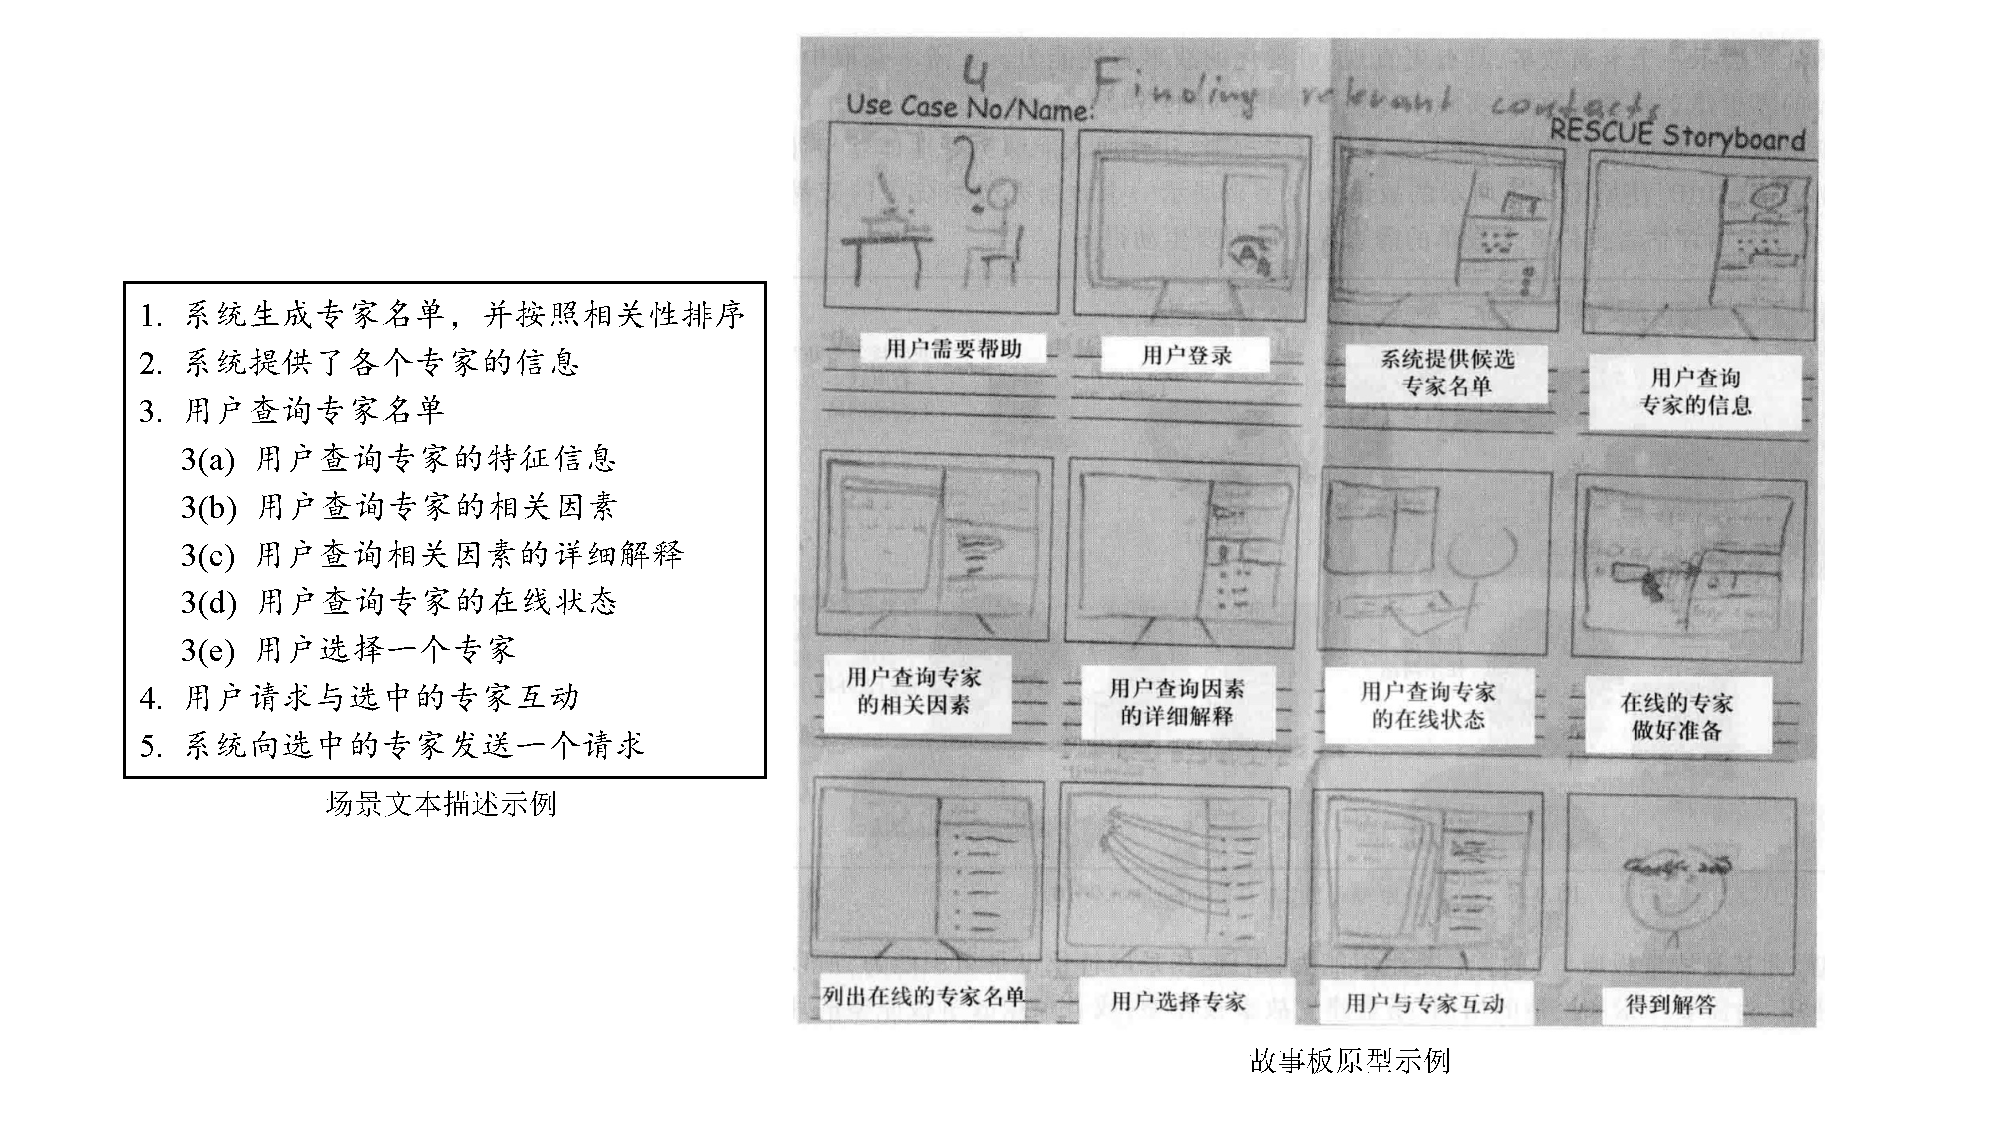
\includegraphics[width=0.83\textwidth]{img/为场景描述建立更直观的故事板原型.pdf}
    \caption*{为场景描述建立更直观的故事板原型}
    \vspace{-1em}
\end{figure}

\subsection{原型方法的风险}
\begin{itemize}
    \item 原型开发工作投入太多的工作,使得开发团队消耗了过多的时间和过大的成本
    \item 涉众看到了一个正在运行的原型,得出产品几乎已经完成的结论,从而提出快速交付产品的不当要求
    \begin{itemize}
        \item 不要将原型的功能开发的太好,以免用户提出“交付”的要求
    \end{itemize}
    \item 用户可能会被原型所表现出来的非功能特性遮蔽了眼睛,从而忽略了他们更应该重视的功能特性
    \item 在澄清需求不确定性的同时也可能会掩盖一些用户的假设,这些假设将会无从发现
\end{itemize}

\subsection{总结}
\begin{itemize}
    \item 原型是软件开发当中消除不确定性风险的有效工具,是一种有效的需求获取方法
    \item 原型的体系是复杂的,不同类型的原型具有不同的作用和创建要求,实践当中应该综合考虑各种应用因素选择合适的类别
    \item 一个完整的原型方法过程可以帮助更有效的应用原型方法
    \item 原型方法的应用可能会给项目带来相应的风险,需要妥善的加以解决
\end{itemize}

	\section{观察与文档审查}

\subsection{观察的情境适用性}
观察应用于用户无法完成主动的信息告知的情况下,目前常见的观察方法有以下几种
\vspace{-0.8em}
\begin{multicols}{3}
    \begin{itemize}
        \item 采样观察
        \item 民族志
        \item 话语分析
        \item 协议分析
        \item 任务分析
    \end{itemize}
\end{multicols}
\vspace{-1em}

某些事件只有和它们发生时的具体环境联系起来,才能得到理解,情景性的重要性质主要有以下几个
\vspace{-0.8em}
\begin{multicols}{2}
    \begin{itemize}
        \item 突现:集体促成 ,互动中突现 
        \item 局部:特定的上下文环境 
        \item 暂时:演进过程中的一刻
        \item 涉身:参与者的认知和能力受限
        \item 开放:业务不确定并开放,以后完善
        \item 模糊:基于潜在知识,尚未明确表达
    \end{itemize}
\end{multicols}
\vspace{-1em}

观察方法对情景性问题的解决
\begin{table}[H]
    \centering
    \begin{tabular}{|c|c|l|}
    \hline
    方法                    & 情景性性质 & \multicolumn{1}{c|}{描述}          \\ \hline
    \multirow{3}{*}{采样观察} & 局部    & 对工作进行一段时间的观察,发现其中的异常处理           \\ \cline{2-3} 
                          & 暂时    & 对实际工作进行观察,发现并纠正其与规章、手册或者用户意识中的不同 \\ \cline{2-3} 
                          & 模糊    & 观察特殊事件的进行,发现用户工作中的潜在知识           \\ \hline
    \multirow{5}{*}{民族志}  & 突现    & 通过观察,分析群体的互动,理解复杂的协同事件           \\ \cline{2-3} 
                          & 局部    & 长时间的观察,可以发现各种情况下的异常处理和特殊情况       \\ \cline{2-3} 
                          & 暂时    & 对实际工作进行观察,发现并纠正其与规章、手册或者用户意识中的不同 \\ \cline{2-3} 
                          & 涉身    & 在观察中学习,了解用户本身的认知和能力              \\ \cline{2-3} 
                          & 模糊    & 了解各种基础的细节,能够发现用户工作中的潜在知识         \\ \hline
    会话分析                  & 涉身    & 通过分析用户交谈发现用户的认知和能力               \\ \hline
    协议分析                  & 模糊    & 发现用户工作中的潜在知识                     \\ \hline
    \end{tabular}
    \vspace{-1em}
\end{table}

观察方法解决的问题
\begin{itemize}
    \item 理解复杂的协同事件:突现,民族志 
    \item 获取工作中的异常处理:局部,采样观察、民族志
    \item 获取与用户认知不一致的实际知识:暂时,采样观察、民族志 
    \item 了解用户的认知:涉身,民族志、话语分析
    \item 获取默认知识:模糊,采样观察、民族志、协议分析
\end{itemize}


\subsection{观察方法的应用}

\subsubsection{采样观察}
\vspace{-0.5em}
\begin{table}[H]
    \centering
    \begin{tabular}{|c|l|l|}
    \hline
    \multicolumn{1}{|l|}{} & \multicolumn{1}{c|}{时间采样}                                                         & \multicolumn{1}{c|}{事件采样}                                               \\ \hline
    优点                     & \begin{tabular}[c]{@{}l@{}}\ding{172}通过随机的观察减少偏差\\ \ding{173}对频繁发生事件取代表性事件进行观察\end{tabular}         & \begin{tabular}[c]{@{}l@{}}\ding{172}允许在行为展开过程中观察\\ \ding{173}允许对指定的重要事件进行观察\end{tabular} \\ \hline
    缺点                     & \begin{tabular}[c]{@{}l@{}}\ding{172}用分段的方式来收集数据不能提供全面信息的时间\\ \ding{173}漏掉不经常发生却很重要的事件\end{tabular} & \begin{tabular}[c]{@{}l@{}}\ding{172}消耗大量时间\\ \ding{173}漏掉频繁发生事件的代表性样本\end{tabular}       \\ \hline
    \begin{tabular}[c]{@{}c@{}}适用\\ 情景\end{tabular}                   & \begin{tabular}[c]{@{}l@{}}\ding{172}发现异常流程\\ \ding{173}验证用户知识和实际工作的一致性\end{tabular}                & \begin{tabular}[c]{@{}l@{}}\ding{172}获取默认知识\\ \ding{173}验证用户知识和实际工作的一致性\end{tabular}      \\ \hline
    \end{tabular}
\vspace{-1em} 
\end{table}

\subsubsection{民族志}
对一些复杂的协同工作而言,工作的协同安排具有一定的社会性,是按照社会化的方式组织的,也就是说复杂的协同 工作具有突现的情景性。民族志可以帮助开发者了解这些工作的社会性因素,解决突现的情景性因素。

民族志的优点
\vspace{-0.8em}
\begin{multicols}{2}
    \begin{itemize}
        \item 能够得到信息的深度理解
        \item 能够让真实世界的社会性因素可见化
        \item 打破人们已有的一些错误假设和错误观念
    \end{itemize}
\end{multicols}
\vspace{-1em}

民族志的缺点
\vspace{-0.8em}
\begin{multicols}{2}
    \begin{itemize}
        \item 需要耗费很多的时间
        \item 调研结果很难传递到开发过程
    \end{itemize}
\end{multicols}
\vspace{-1em}

在民族志当中,需求工程师和开发者需要关注3方面的内容
\begin{itemize}
    \item 工作的分布式协同(Distributed Coordination)
    \begin{itemize}
        \item 要特别注意那些利用物件实现的协同和创建这些物件的文书工作
    \end{itemize}
    \item 工作的计划和程序(Plans and Procedures)
    \begin{itemize}
        \item 关注它们在组织活动中的应用方式
        \item 发现实际工作和文档化程序之间存在的偏离
    \end{itemize}
    \item  工作的意识(Awareness of Work)
    \begin{itemize}
        \item 活动是如何对协同中的其他人可见或者可理解的?
    \end{itemize}
\end{itemize}

适用普通民族志的规则
\vspace{-0.8em}
\begin{multicols}{2}
    \begin{itemize}
        \item 应该定期的记录发现 
        \item 尽快的记录可能会在观察过程中发生的面谈 
        \item 定期的复查和更新自己的想法 
        \item 确定管理海量数据的应对策略 
    \end{itemize}
\end{multicols}
\vspace{-1em}

\subsection{文档审查方法的应用}
\begin{table}[H]
    \vspace{-0.5em}
    \centering
    \begin{tabular}{|c|c|l|}
    \hline
    文档类型                                                   & 文档审查方法 & \multicolumn{1}{c|}{描述}                                                                                               \\ \hline
    \begin{tabular}[c]{@{}c@{}}相关产品的需求\\ 规格说明\end{tabular} & 需求重用   & \begin{tabular}[c]{@{}l@{}}分析相关产品的规格说明,发现可以移植到到\\ 新产品中的需求信息,进行需求的重用\\ $\bullet$\ 问题域信息\\ $\bullet$\ 用户界面特征\\ $\bullet$\ 业务需求、组织策略、政策法规\end{tabular} \\ \hline
    硬数据                                                    & 文档分析   & \begin{tabular}[c]{@{}l@{}}阅读、研究得到的硬数据,从中发现需求信息\\ $\bullet$\ 问题域信息\\ $\bullet$\ 工作流程\\ $\bullet$\ 业务细节\end{tabular}                                 \\ \hline
    客户的需求文档                                                & 需求剥离   & \begin{tabular}[c]{@{}l@{}}抽取客户的需求文档中的需求描述\\ $\bullet$\ 粗粒度需求\end{tabular}                                                      \\ \hline
    \end{tabular}
    \vspace{-1em}
\end{table}

\vspace{-0.5em}
\begin{shaded}

\subsubsection*{附:硬数据及硬数据采样}

人们在进行实际工作时会产生各种各样的表格和文档资料,这些表格和文档资料往往是用户对实际业务进行加工和抽象之后的结果,是一种精化过的知识。因此,在研究一个现有系统时,有经验的需求工程师总是会从现有文档中获取事实,理解问题域。这些文档资料被称为硬数据。

[Kendall 2002]将常见的硬数据分为定量硬数据和定性硬数据两种类型
\begin{itemize}
    \item 定量硬数据
    \begin{itemize}
        \item 数据收集表格
        \begin{itemize}
            \item 反映了组织的信息流 
            \item 收集正在使用的每张空白表格表格、填写和分发说明 
            \item 对比填写好的表格
            \begin{itemize}
                \item 表格中是否有从来都不填写的数据项
                \item 应该收到表格的人是否真的收到了
                \item 他们是否按照正常程序使用、存储和丢弃表格
            \end{itemize}
        \end{itemize}
        \item 统计报表
        \begin{itemize}
            \item 反映了组织过去的主要业务和业务目标
            \item 统计规则也是一种丰富的知识,统计项分解为细节业务数据的过程往往也就是组织目标分解到具体业务的过程
            \item 根据实际工作填写过的统计报表,就可以发现组织实际的业务执行状况,从中发现组织面临的具体问题  
        \end{itemize}
    \end{itemize}
    \item 定性硬数据
    \begin{itemize}
        \item 整个组织的描述文档 
        \begin{itemize}
            \item 组织结构图:帮助发现项目的关键涉众
            \item 门户网站:反映组织的业务开展状况
        \end{itemize}
        \item 业务指导文档
        \begin{itemize}
            \item  工作指南和规章手册:解释业务的详细执行过程,反映业务的具体细节
        \end{itemize}
        \item 业务备忘
        \begin{itemize}
            \item 反映业务的实际执行情况
            \item 形成对组织工作过程的清晰理解
        \end{itemize}
    \end{itemize}
\end{itemize}

抽样时样本大小的选择取决于需求工程师希望样本具有多大的代表性。用于确定样本大小($SS$)的一个简单而有效的公式是
$$SS = p\times (1-p) \times \mbox{(确定性因子/可接受的错误)}^2$$
其中$p$是差异样本比例,未知的情况下设为$0.25$

\begin{wraptable}{r}{6.5cm}
    \centering
    \vspace{-1.5em}
    \begin{tabular}{|c|c|}
    \hline
    期望的确定性 & 确定性因子 \\ \hline
    95\% & 1.960  \\ \hline
    90\% & 1.645  \\ \hline
    85\% & 1.281  \\ \hline
    \end{tabular}
    \caption*{常见的确定性因子}
    \vspace{-3em}
\end{wraptable}

例:采样数量示例
\begin{itemize}
    \item 每10张发票中就有1张发票与常规情况不同 
    \item 希望发票样本中包含所有的情况具有90\%的确定性 
\end{itemize}
则选取的样本大小为样本大小为$SS=0.10\times (1-0.10)\times(1.645/0.10)^2=25$

如何选择这25张发票呢?两种常用的抽样技术是随机抽样和分层抽样。随机抽样随机地采样数据,因此,只是根据上面计算出的样本大小随机选择25张发票即可。分层抽样是一种有考虑的系统的方法,试图降低采样数据的方差。例如,假设发票的总数是250000张,由于样本大小需要包括25发票,所以就可以将所有的发票分为25层,每层10000张,最后从每一层中随机抽取一个样本即可。
\end{shaded}
\vspace{-1em}


	\section{需求分析概述}

\subsection{需求分析的根本任务}

\begin{figure}[H]
	\centering
    \vspace{-1em}
	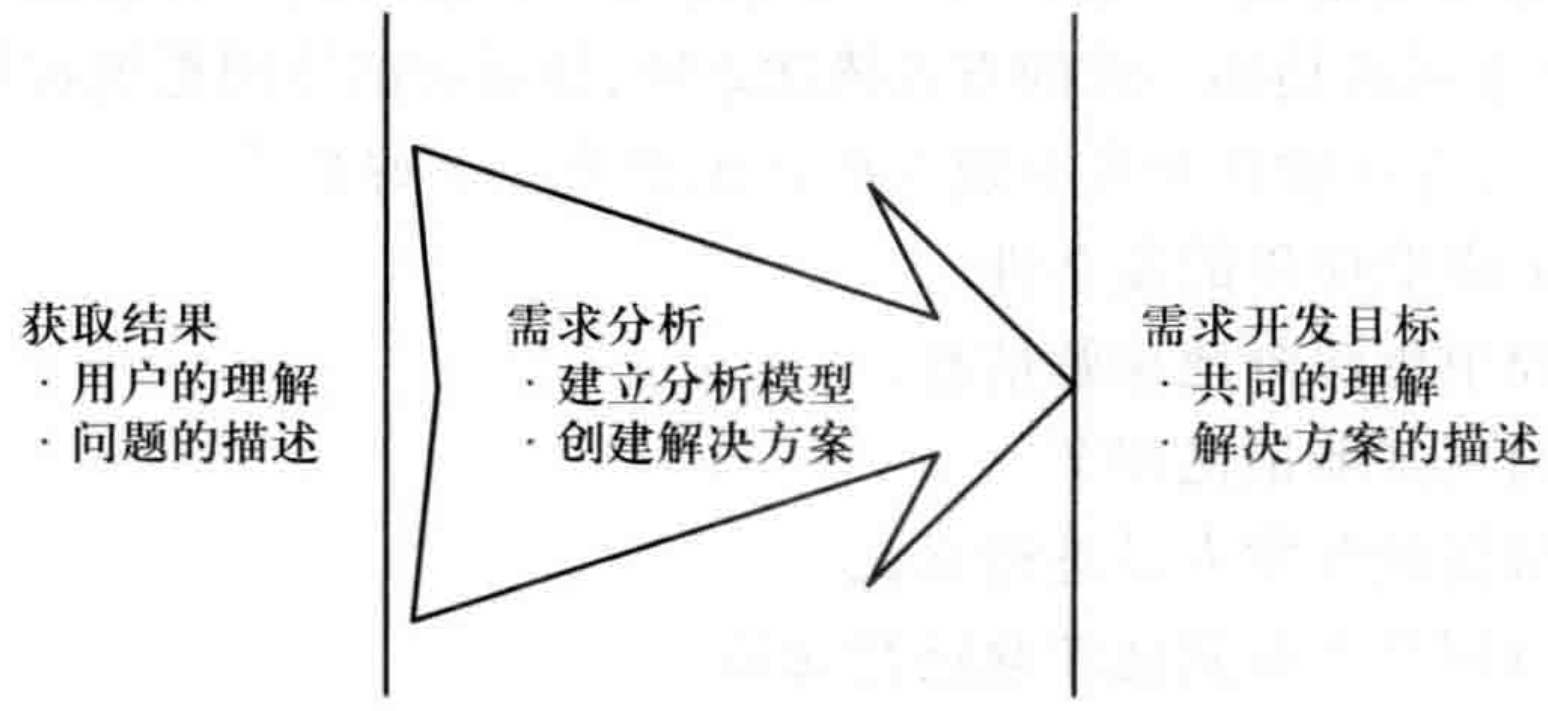
\includegraphics[width=0.55\textwidth]{img/需求分析的任务.png}
    \vspace{-1em}
\end{figure}

需求分析的根本任务有如下两条:
\begin{itemize}
    \item 建立分析模型
    \begin{itemize}
        \item 将复杂的系统分解成为简单的部分以及它们之间的联系,确定本质特征
        \item 和用户达成对信息内容的共同理解
        \item 分析的活动主要包括识别、定义和结构化,它的目的是获取某个可以转换为知识的事物的信息
    \end{itemize}
    \item 创建解决方案
    \begin{itemize}
        \item 将一个问题分解成独立的、更简单和易于管理的子问题来帮助寻找解决方案
        \item 创建解决方案的过程是创造性的
        \item 帮助开发者建立问题的定义,并确定被定义的事物之间的逻辑关系
        \begin{itemize}
            \item 这些逻辑关系可以形成信息的推理,进而可以被用来验证解决方案的正确性
        \end{itemize}
    \end{itemize}
\end{itemize}

\subsubsection{建立分析模型}

\paragraph{模型}~{} \par
“模型是对事物的抽象,帮助人们在创建一个事物之前可以有更好的理解” 

集中关注问题的计算特性(数据、功能、规则等等) 

“它是对系统进行思考和推理的一种方式。建模的目标是建立系统的一个表示,这个表示以精确一致的方式描述系统,使得系统的使用更加容易” 

建模方法
\begin{itemize}
    \item 抽象(Abstraction)
    \begin{itemize}
        \item 一方面要求人们只关注重要的信息,忽略次要的内容:通过强调本质的特征,就减少了问题的复杂性
        \item 另一方面也要求人们将认知保留在适当的层次,屏蔽更深层次的细节:在问题的各元素之间推断出更广泛和更普遍的关系,帮助人们寻找解决方案
    \end{itemize}
    \item 分解(Decomposition/Partitioning)
    \begin{itemize}
        \item “分而治之”:将单个复杂和难以理解的问题分解成多个相对更容易的子问题,并掌握各子问题之间的联系
        \item 分解的方案往往还能提供问题的解决思路
    \end{itemize}
    \item 投影(Projection)
    \begin{itemize}
        \item 多视点方法
    \end{itemize}
\end{itemize}

\paragraph{两个世界与三种模型}~{} \par
\textbf{计算世界与计算模型} \par
基于软件构建单位及其之间的关系建立的模型是软件工程中非常常用的一种模型形式,用来说明软件逻辑上的构建方式和实现方式。这种模型使用的组元及其关系都是软件的元素,所以它是来自于软件(计算世界)的模型,称为计算模型。

基于计算科学建立的,具有形式化的特征
\begin{itemize}
    \item 信息的描述具有明确化、准确化和确定化的特征
\end{itemize}

需求分析阶段不适宜建立形式化的计算模型
\vspace{-0.8em}
\begin{multicols}{2}
    \begin{itemize}
        \item 重点是问题,缺乏和软件实现相关的技术细节
        \item 用户无法理解
    \end{itemize}
\end{multicols}
\vspace{-1em}

\begin{figure}[H]
	\centering
    \vspace{-0.5em}
	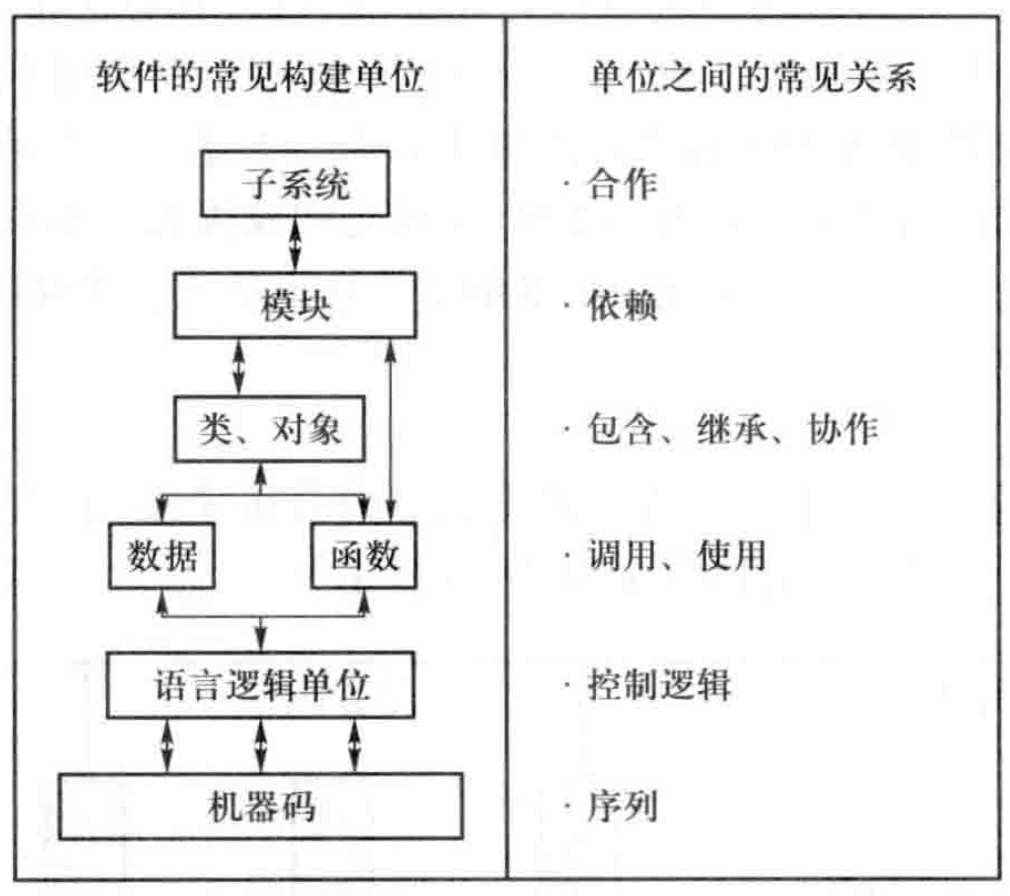
\includegraphics[width=0.53\textwidth]{img/软件的常见构建单位及其关系.png}
    \caption*{软件的常见构建单位及其关系}
    \vspace{-1em}
\end{figure}


\textbf{问题世界与业务模型} \par
业务模型使用问题域中的重要概念作为模型的组元,使用概念之间的业务联系作为组元之间的关系

使用了业务描述的方式,具有非形式化特征
\begin{itemize}
    \item 业务模型元素(即业务概念和业务联系)的选取和定义上具有不准确、不确定和模糊化
    \item 可以抽取出需求信息中最重要和最本质的内容
    \item 可以达成用户和开发者的共同理解
\end{itemize}

非形式化特征使得它不适合于进行需求建模
\begin{itemize}
    \item 不足以用于描述一个有效的软件解决方案:不准确、不确定和模糊化
\end{itemize}

\textbf{软件分析模型} \par
软件分析模型是介于计算模型和业务模型二者之间的模型形式,使用了计算模型的组元形式,在组元的表现上采用了业务模型的表现方式

\begin{figure}[H]
	\centering
    \vspace{-0.5em}
	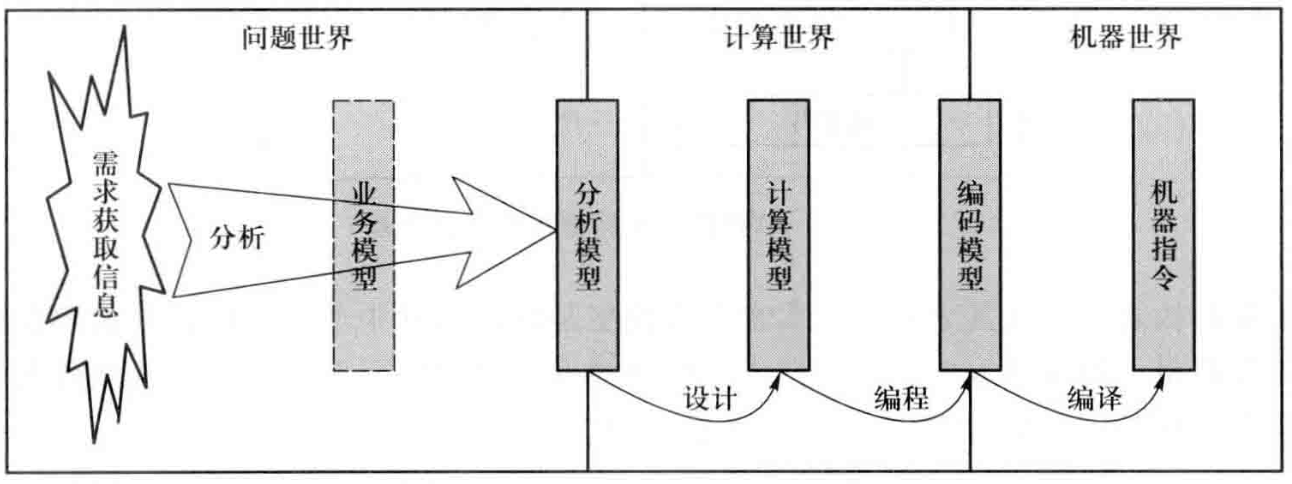
\includegraphics[width=0.75\textwidth]{img/软件分析模型.png}
    \caption*{软件分析模型}
    \vspace{-1em}
\end{figure}

软件分析模型是半形式化的,不再像计算模型那么严谨,不再具有形式化的特征,由于需求分析的半形式化特征还使得它可以比业务模型更严格

\textbf{三种模型的区别示例} \par
\begin{figure}[H]
	\centering
    \vspace{-0.5em}
	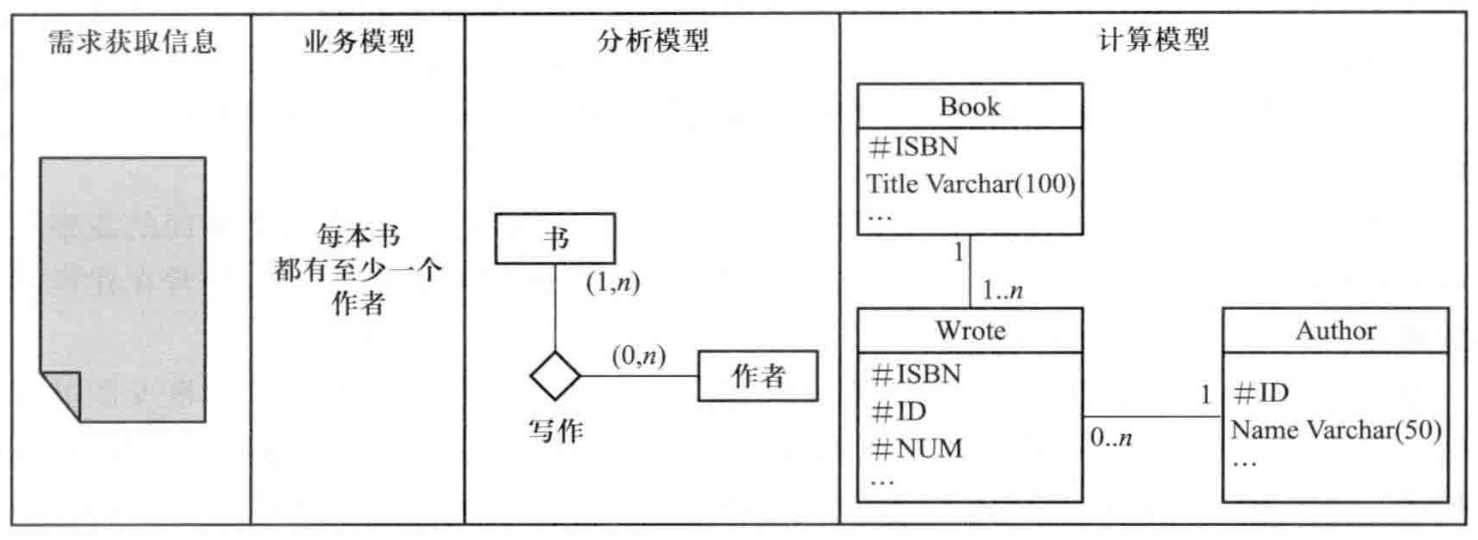
\includegraphics[width=0.75\textwidth]{img/3种模型的区别示例.png}
    \vspace{-1em}
\end{figure}

\paragraph{需求建模}~{} \par
需求建模通常的做法是:
\begin{itemize}
    \item 先依据获取的问题域信息建立初步的模型
    \item 然后分析用户需求,对模型进行调整,得到一个中间形式的模型形式
    \item 最后,对调整后的模型进行逻辑推理和验证,如果符合预期的期望,那么它就是最终的解决方案模型
\end{itemize}

\begin{figure}[H]
	\centering
    \vspace{-0.5em}
	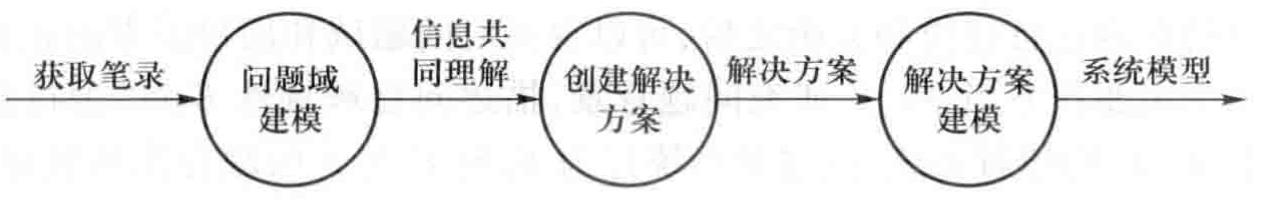
\includegraphics[width=0.7\textwidth]{img/需求建模过程.png}
    \caption*{需求建模过程}
    \vspace{-1em}
\end{figure}


\subsubsection{建立解决方案}
\begin{figure}[H]
	\setcounter{subfigure}{0}
	\centering
	\vspace{-1em}	
	\subfloat{
		\begin{minipage}[c]{0.48\linewidth}
		\centering
		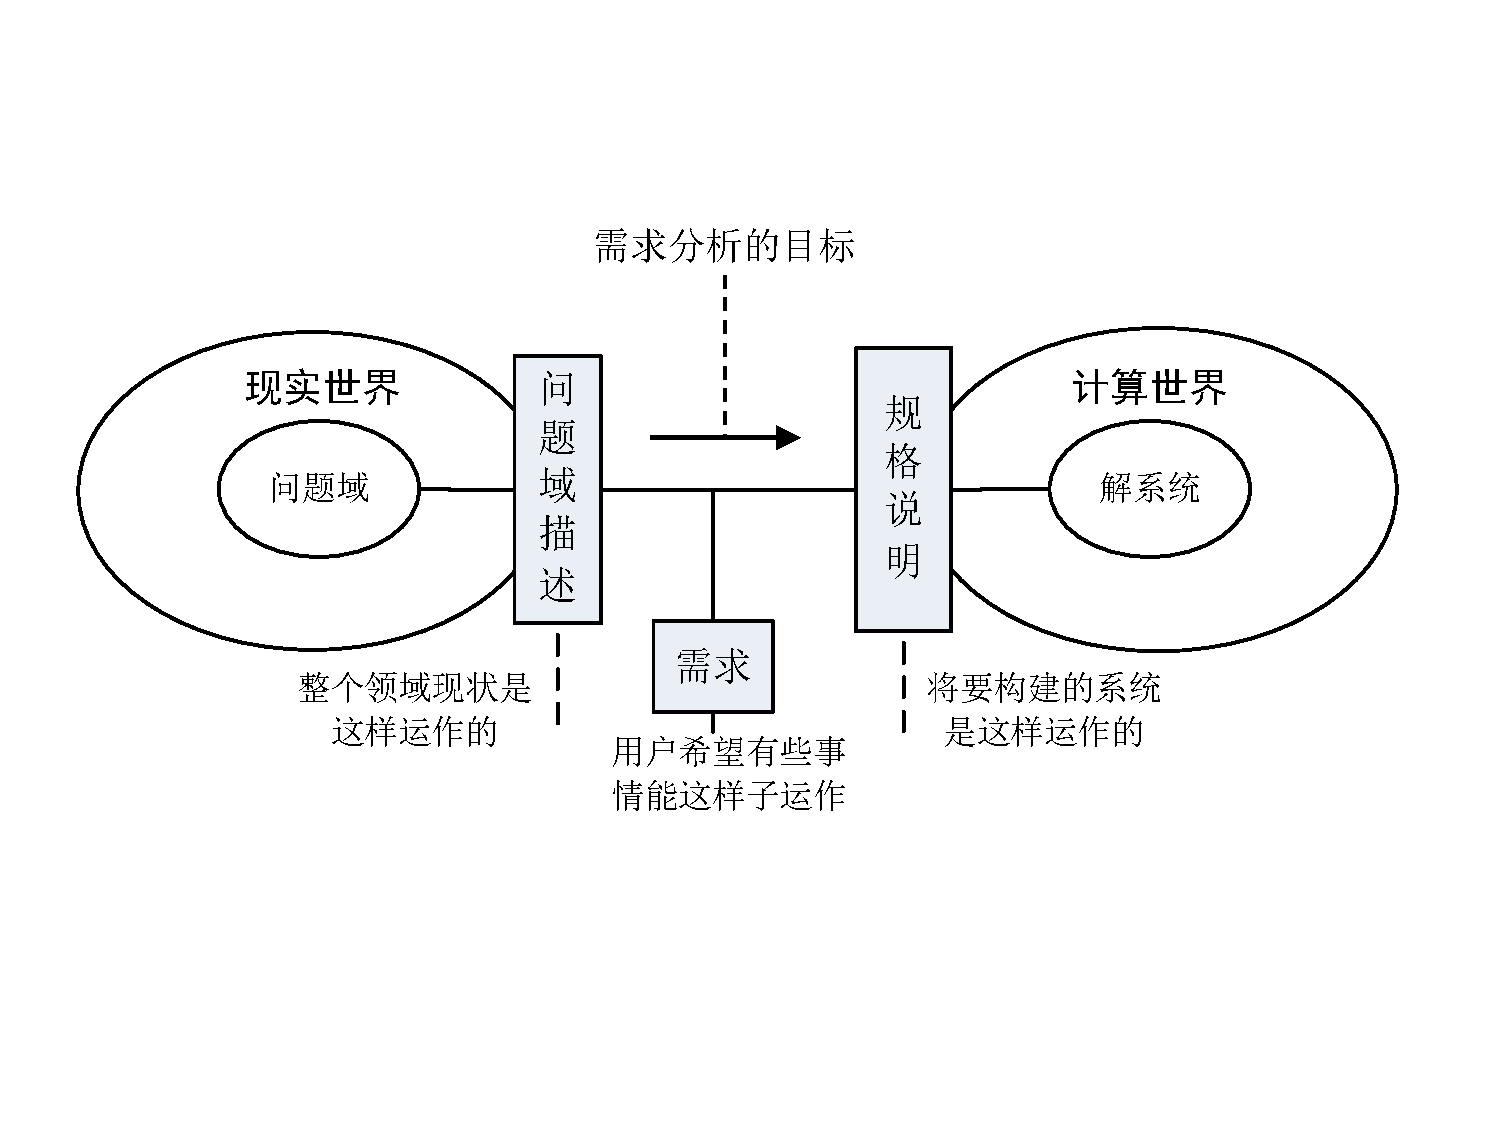
\includegraphics[width=\linewidth]{img/建立解决方案.pdf}
		\end{minipage}
	}
	\subfloat{
		\begin{minipage}[c]{0.49\linewidth}
		\centering
		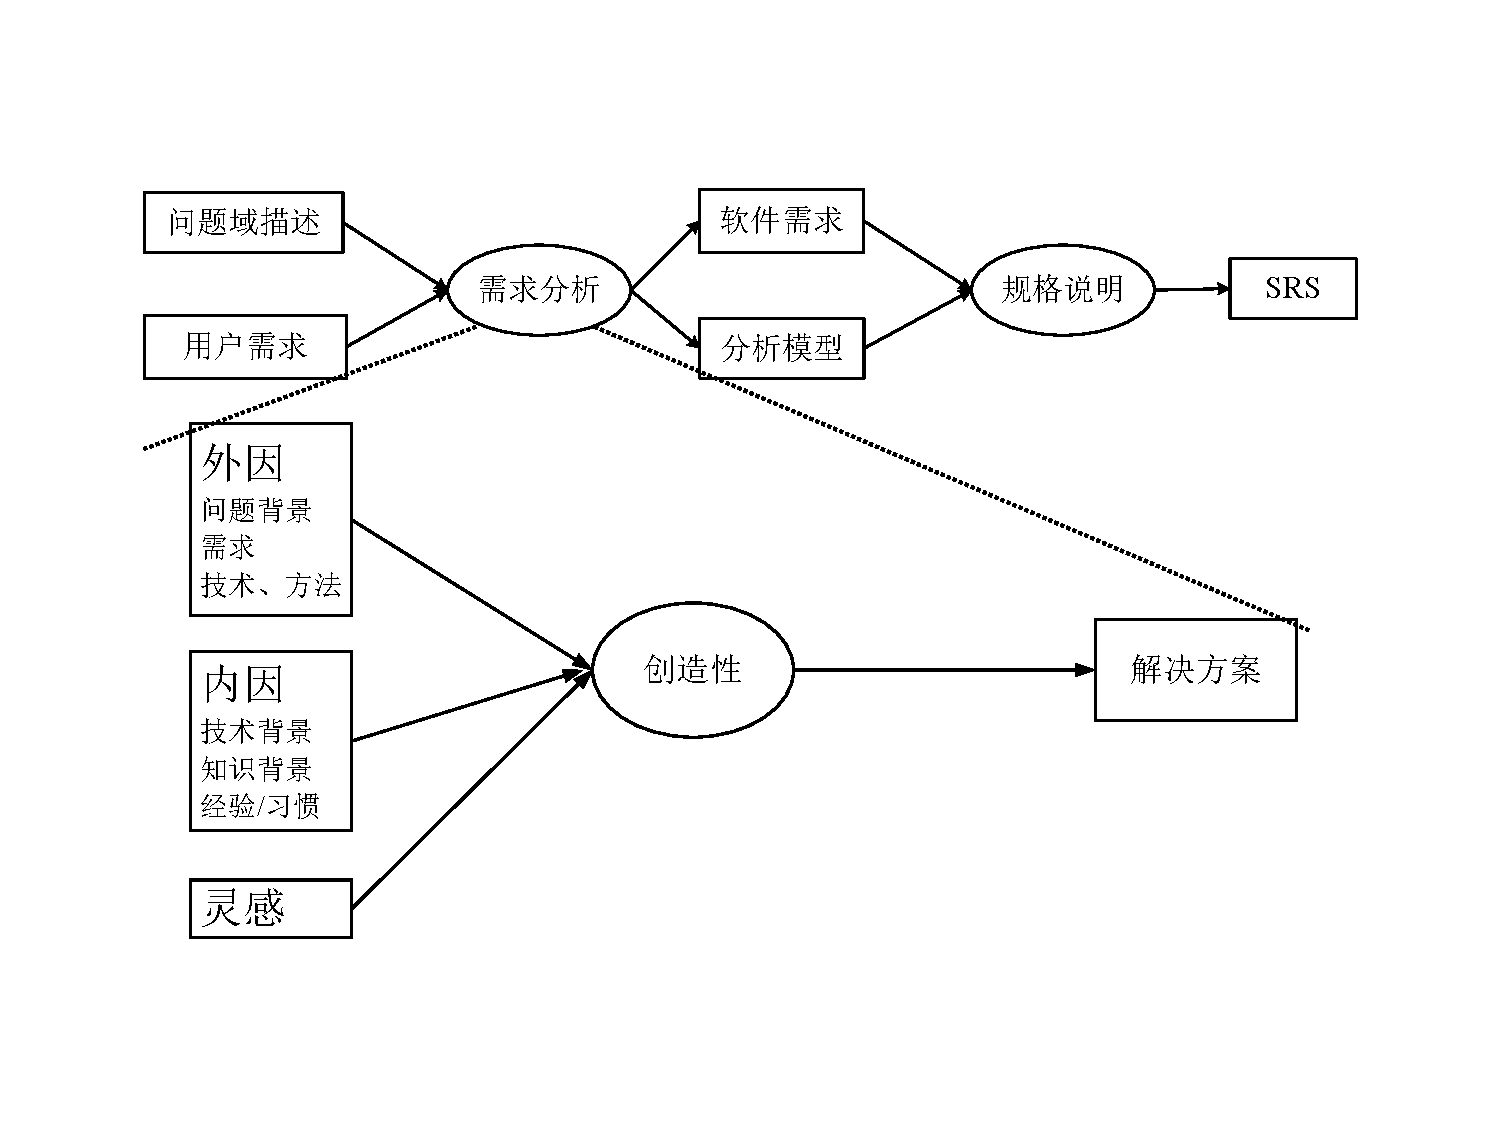
\includegraphics[width=\linewidth]{img/建立解决方案的过程.pdf}
		\end{minipage}
	}
	\centering
	\vspace{-1em}
\end{figure}

\subsection{需求分析方法}
\begin{figure}[H]
	\centering
    \vspace{-0.5em}
	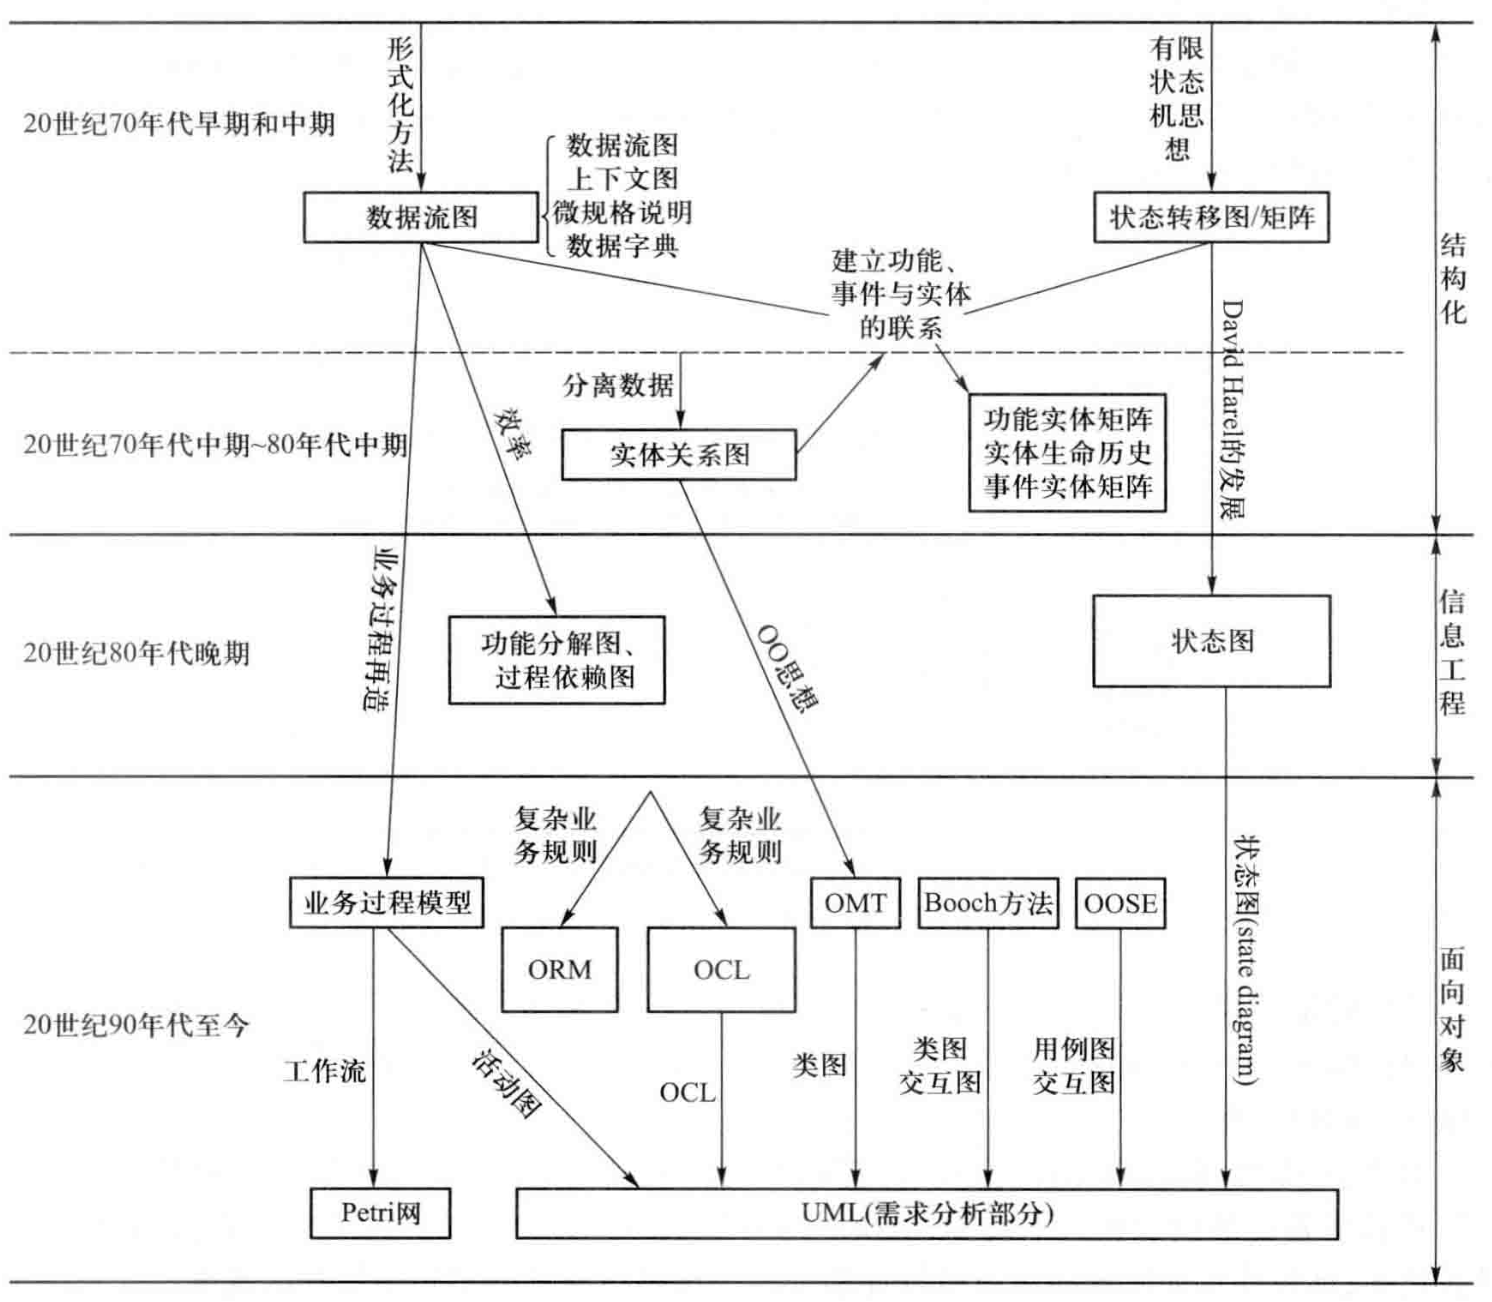
\includegraphics[width=0.9\textwidth]{img/常见需求分析技术的发展历程.png}
    \caption*{常见需求分析技术的发展历程}
    \vspace{-1em}
\end{figure}

\begin{figure}[H]
	\setcounter{subfigure}{0}
	\centering
	\vspace{-1em}	
	\subfloat{
		\begin{minipage}[c]{0.56\linewidth}
		\centering
		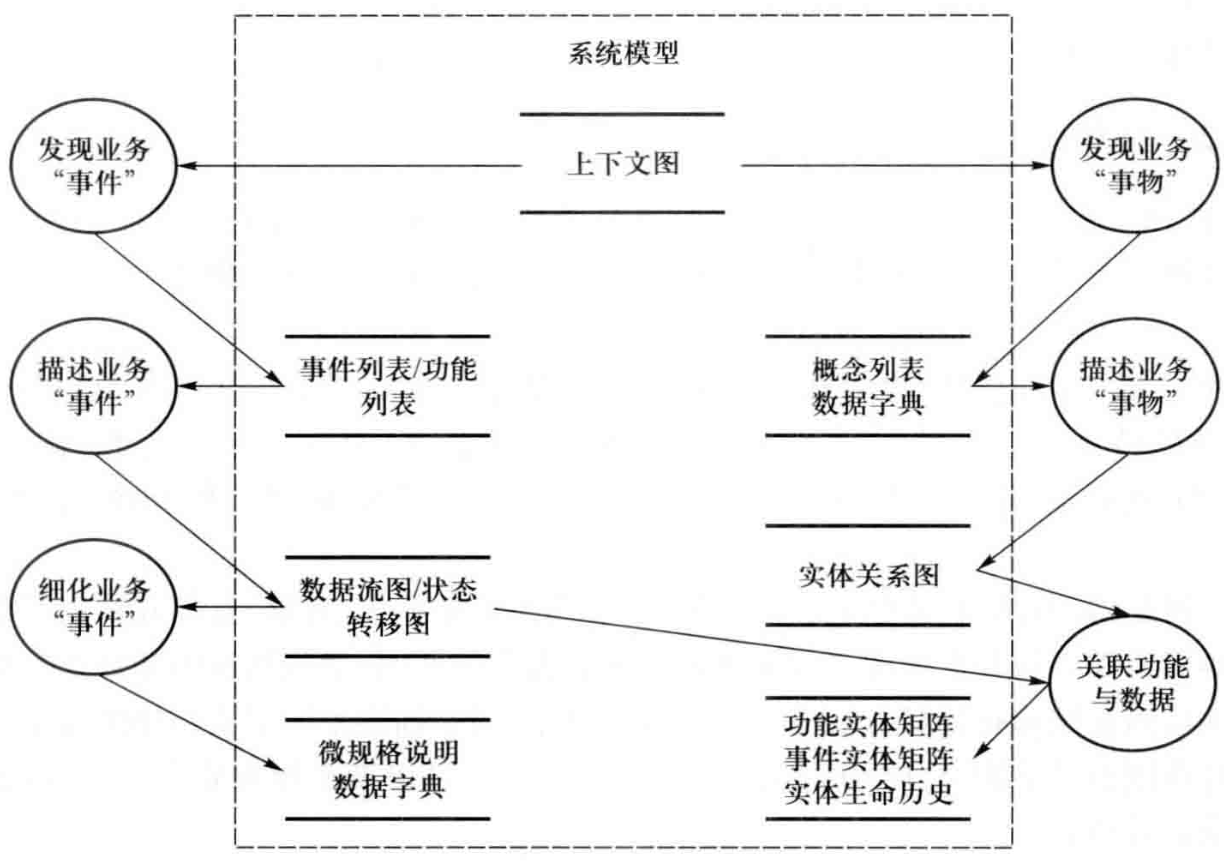
\includegraphics[width=\linewidth]{img/结构化分析的典型过程.png}
        \caption*{结构化分析的典型过程}
		\end{minipage}
	}
	\subfloat{
		\begin{minipage}[c]{0.37\linewidth}
		\centering
		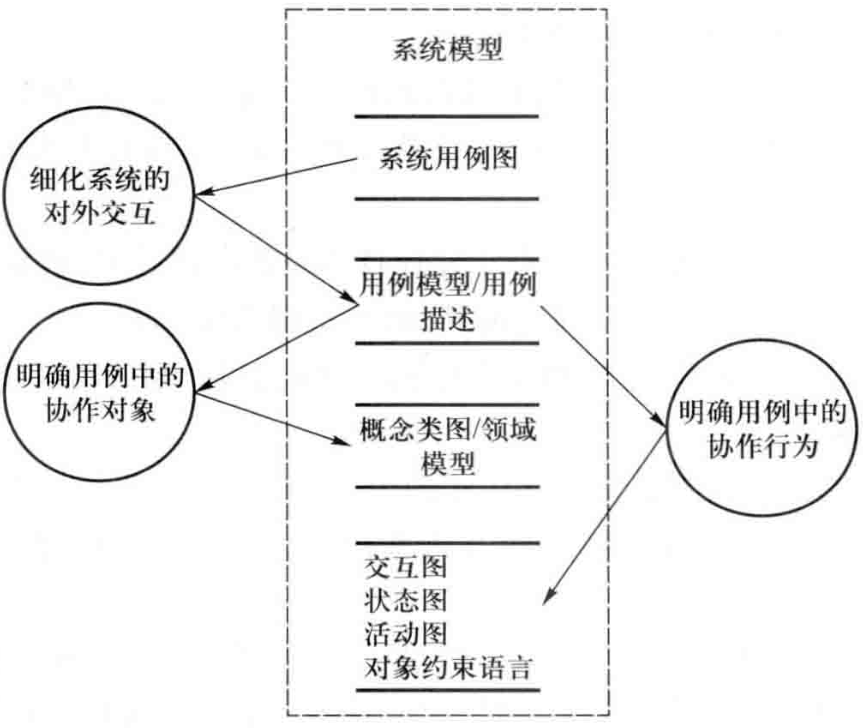
\includegraphics[width=\linewidth]{img/面向对象分析的典型过程.png}
        \caption*{面向对象分析的典型过程}
		\end{minipage}
	}
	\centering
	\vspace{-1em}
\end{figure}


\subsection{需求分析的活动}
\begin{figure}[H]
	\centering
    \vspace{-0.5em}
	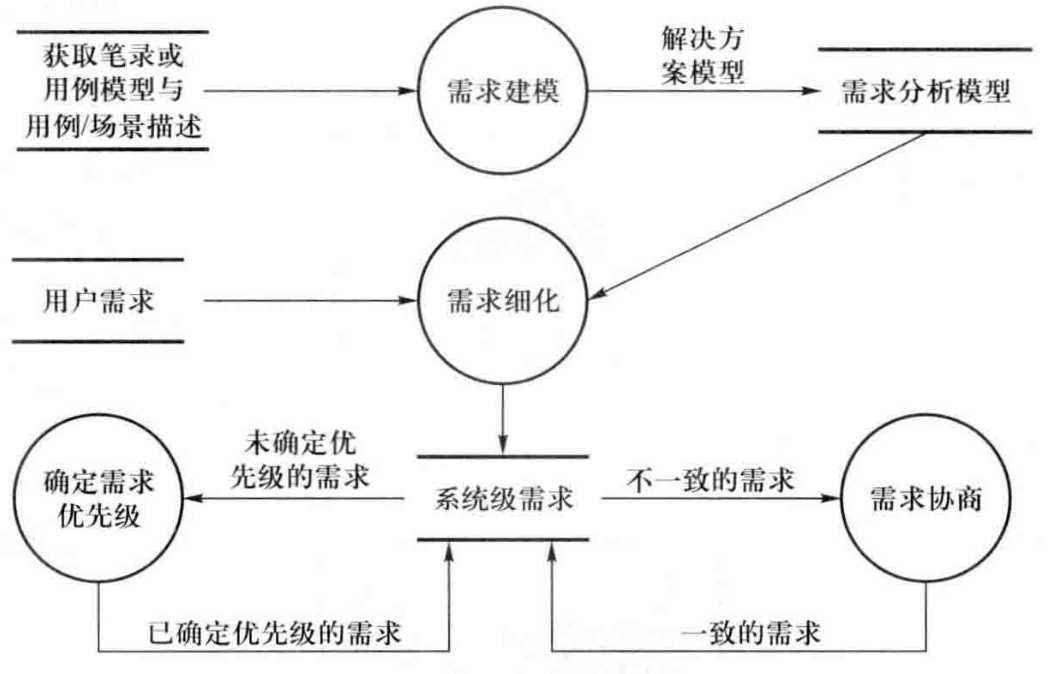
\includegraphics[width=0.65\textwidth]{img/后期需求阶段的需求分析活动流程图.png}
    \caption*{后期需求阶段的需求分析活动流程图}
    \vspace{-1em}
\end{figure}

\subsubsection{需求细化}
\begin{itemize}
    \item 明确用户需求的隐含因素 
    \item 将从问题域和业务的角度表述的用户需求等价的转化为从软件和技术的角度表述的系统需求 
    \item 非功能需求也需要从高层次的表述方式转化为一系列更加详细和具体的需求表述 
    \item 需求细化也会发现新的细节需求
    \item 需求已经得了充分的理解,并且开发者已经可以着手为其进行方案设计时停止细化过程 
    \item 细化后的需求应该被一一的标识和记录下来 
\end{itemize}

在分析活动当中需要收集每条需求的重要属性,常见的属性有以下几种
\vspace{-0.8em}
\begin{multicols}{2}
    \begin{itemize}
        \item 标识符,每一条需求都应该能够通过ID唯一的标识自己
        \item 源头,要能回溯到需求源头,例如特定的涉众
        \item 理由,需求被提出的目的
        \item 优先级,详细情况见下一节
        \item 成本,预估的实现成本
        \item 风险,实现该需求的过程中可能带来的风险
        \item 可变性,将来发生变化的可能性
    \end{itemize}
\end{multicols}

\subsubsection{确定需求优先级}
确定需求优先级的常用方法有下列几种:累计投票、区域划分、Top$-N$和数据量化

\textbf{累计投票:}在这种方法下,所有参与需求优先级评定的人员都会在一开始被给予一定数量的投票分数(如100分)。然后评定人员根据自己的判断将这些分数分配给各个单独的需求。最后,将每个需求得到的投票分值汇总,得到的总分值就代表了该需求的优先级,分值越大的需求优先级越高。

\textbf{区域划分:}在这种方法下,会将用来评价优先级的特征分为几个等级, 然后建立不同的优先级区域。最后,由评价人员将需求划分到不同的区域当中,每个区域的优先级等级就是该区域内所有需求的优先级。

\begin{table}[H]
    \centering
    \begin{tabular}{|c|c|c|}
    \hline
     & 重要 & 不重要 \\ \hline
    紧急 & 高优先级 & 不予处理 \\ \hline
    不紧急 & 中优先级 & 低优先级 \\ \hline
    \end{tabular}
    \vspace{-0.3em}
    \caption*{区域划分方法示例}
    \vspace{-1em}
\end{table}

可以用来评价优先级的常见特征有以下几方面
\vspace{-0.8em}
\begin{multicols}{2}
    \begin{itemize}
        \item 重要性。需求的不可或缺程度。
        \item 紧急性。需求的时间紧迫程度。
        \item 惩罚性。忽略需求会导致的惩罚程度。
        \item 成本。实现需求的代价。
        \item 风险。需求实现中可能产生的风险程度。 
    \end{itemize}
\end{multicols}
\vspace{-1em}

$\mathbf{Top}-\symbfit{N}$\textbf{:}这通常是在迭代式开发中使用的方法,如敏捷开发。在这种方法下,于每次迭代开始之前,由评价人选择他们认为最为重要的$N$个需求。这里$N$的取值是不受明确限制的,真正受限制的是Top $-N$个需求的实现代价总和。

\textbf{数据量化:}这种方法会将评价优先级的特征量化,然后再依据一定的计算规则计算需求最终的优先级。
\vspace{-0.3em}
$$\mbox{优先级}=\frac{\mbox{价值}\%}{(\mbox{成本\%}\times \mbox{成本权值}) + (\mbox{风险}\% \times \mbox{风险权值})}$$

\begin{figure}[H]
	\centering
    \vspace{-0.8em}
	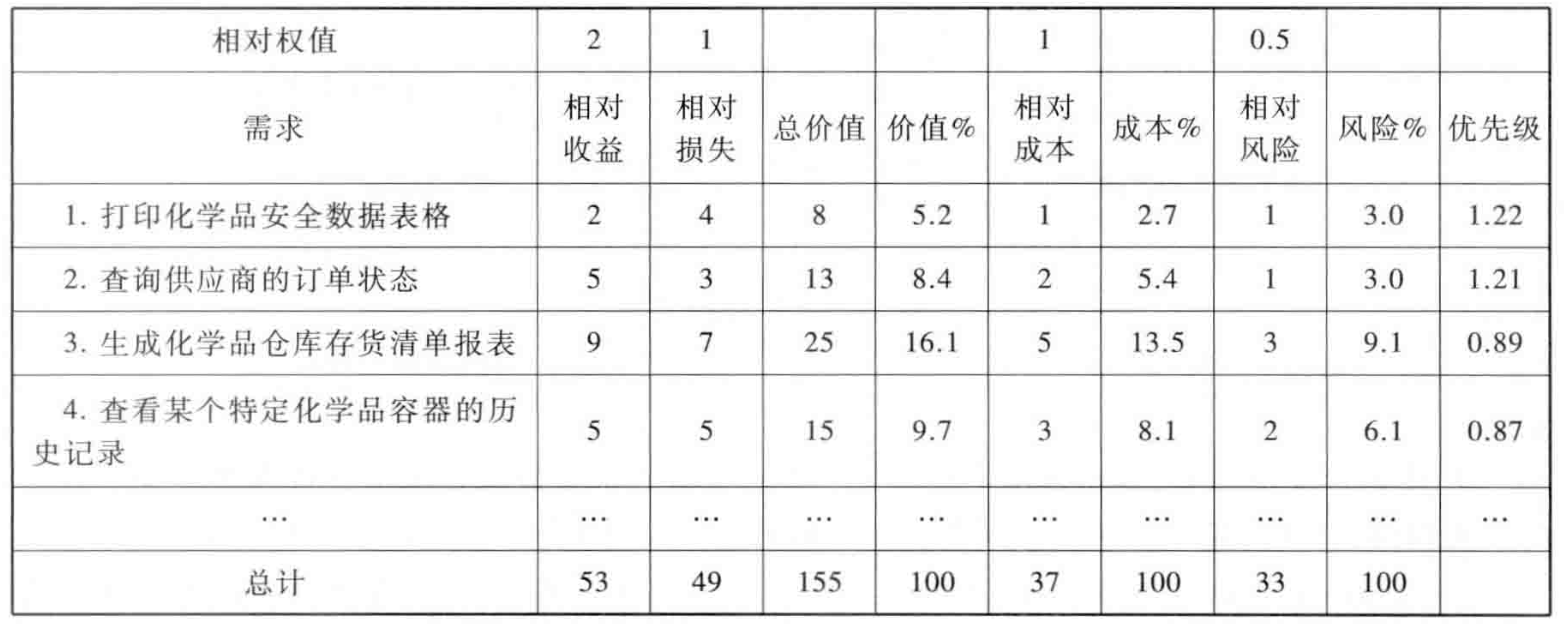
\includegraphics[width=0.85\textwidth]{img/QFD方法示例.png}
    \vspace{-1em}
\end{figure}

\vspace{-0.5em}
\begin{shaded}
    
\textbf{用户故事地图:}基于时间延迟成本的优先级判断
\begin{itemize}
    \item 延迟成本相同,短任务优先
    \item 工作量相同,高延迟成本优先
    \item 加权最短任务优先(重要$+$紧急程度)
    \item 所有优先级都是本地和临时的
\end{itemize}

\begin{figure}[H]
	\centering
    \vspace{-0.8em}
	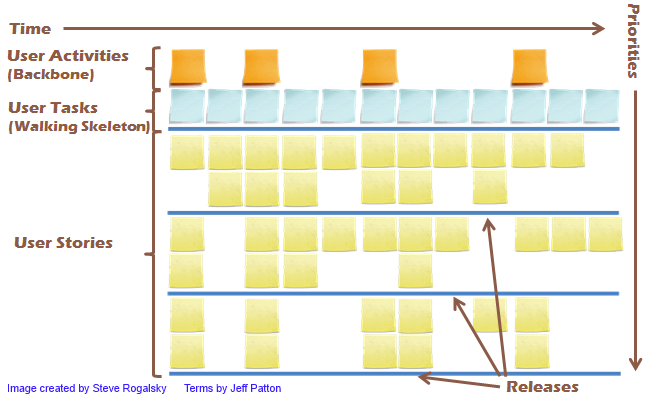
\includegraphics[width=0.6\textwidth]{img/用户故事地图.png}
    \vspace{-1em}
\end{figure}

\end{shaded}
\vspace{-1em}

\subsubsection{需求协商}
需求协商当中应该子以确保的3个原则
\vspace{-0.8em}
\begin{multicols}{2}
    \begin{itemize}
        \item 明确冲突的因素,避免情绪上的冲突
        \item 明确冲突的解决空间
        \item 确定最佳解决方案 
    \end{itemize}
\end{multicols}
\vspace{-1em}

\begin{figure}[H]
	\centering
    \vspace{-0.8em}
	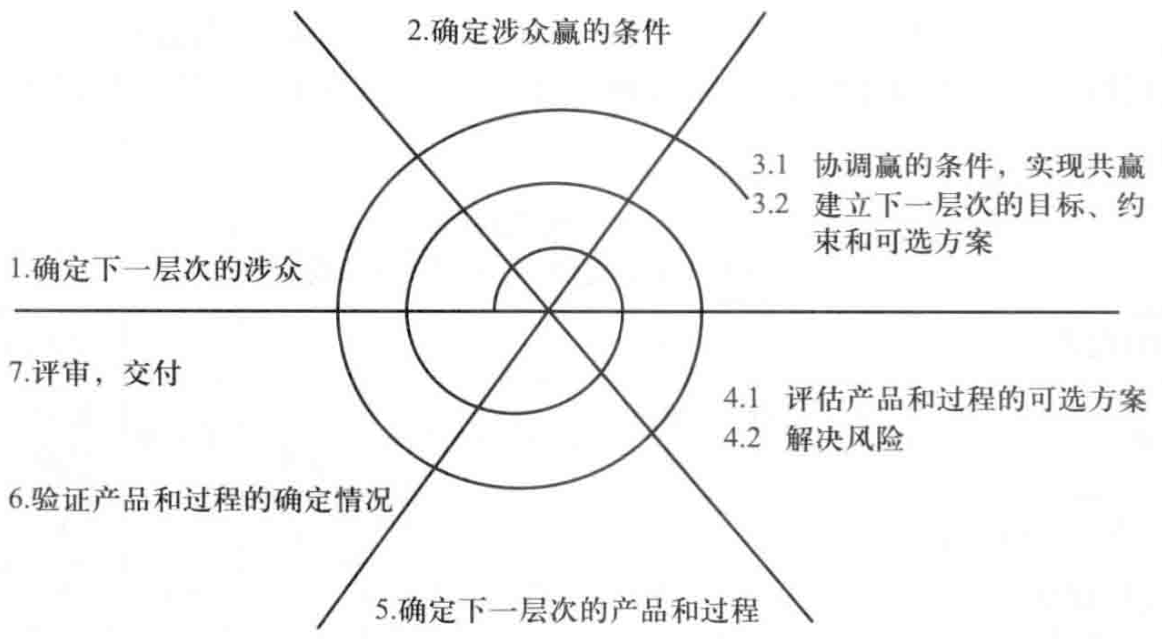
\includegraphics[width=0.67\textwidth]{img/WinWin螺旋模型.png}
    \caption*{WinWin螺旋模型}
    \vspace{-1em}
\end{figure}

	\section{面向对象建模}

\subsection{面向对象分析}

\subsubsection{现实世界的复杂模型}
\begin{itemize}
    \item 复杂总是简单部分的组合
    \item 简单部分又是更简单部分的组合
    \begin{itemize}
        \item 简单组成复杂的过程存在层次性
    \end{itemize}
    \item 每个最小简单部分独立负责完成一系列相关任务
    \item 相比较而言,每个组合内部各部分的关系比其内部与外部的关系都更紧密
    \item 各个部分通过一致的接口进行组合,即一个部分对其它部分的所知仅仅是接口
\end{itemize}

\subsubsection{映射现实模型的面向对象思想}
\begin{itemize}
    \item 任何系统都是能够完成一系列相关目标和任务的对象
    \begin{itemize}
        \item 对象完成一个任务时会请求一系列其他对象帮助其完成一些子目标
        \item 其他对象为了完成其任务又会请求将子目标更细分为子子目标,并请求其他对象帮助完成
        \item 子目标的分解和责任分担一直进行直到最后产生的子部分可以映射到计算实体
    \end{itemize}
\end{itemize}

\vspace{-0.8em}
\begin{multicols}{3}
    \begin{itemize}
        \item 计算实体:对象
        \item 层次关系:继承/关联、聚合/组合
        \item 组合接口:一个对象暴露的接口
    \end{itemize}
\end{multicols}
\vspace{-1em}

\subsubsection{基于UML的面向对象分析}
UML是以Booch方法、OOSE方法和ONT方法为基础,发挥3种方法的互补性,互相取长补短,并吸收了对象约束语言(Object Constraint Language, OCL)等其他技术之后产生的。
\begin{figure}[H]
	\centering
    \vspace{-0.5em}
	\includegraphics[width=0.7\textwidth]{img/Booch方法、OOSE方法、OMT方法与UML.png}
    \caption*{Booch方法、OOSE方法、OMT方法与UML}
    \vspace{-1em}
\end{figure}

在需求分析中涉及的UML技术有:
\vspace{-0.8em}
\begin{multicols}{2}
    \begin{itemize}
        \item 用例图(用例模型)
        \item 类图(对象模型)
        \item 交互图(顺序图/通信图,行为模型-对象协作)
        \item 状态图(行为模型-状态机)
        \item 活动图(行为模型-业务过程)
        \item 对象约束语言OCL
    \end{itemize}
\end{multicols}
\vspace{-1em}

面向对象分析与设计的关键是实现从用例模型到完全对象模型的过渡,包括下列几个步骤:
\begin{figure}[H]
	\centering
    \vspace{-0.5em}
	\includegraphics[width=0.9\textwidth]{img/面向对象方法的技术路线.png}
    \caption*{面向对象方法的技术路线}
    \vspace{-1em}
\end{figure}

\subsection{对象模型}

\subsubsection{对象}
对象是指在一个应用当中具有明确角色的独立可确认的实体 

每个对象都要包含
\begin{itemize}
    \item 标识:唯一的标识自己,对象模型使用对象的引用作为对象的标识
    \item 状态:对象的特征描述,包括对象的属性和属性的取值 
    \item 行为:对象在其状态发生改变或者接收到外界消息时所采取的行动 
\end{itemize}

常见的事物都可以是对象
\begin{itemize}
    \item 和系统存在交互的外部实体,例如人、设备、其他的软件系统等
    \item 问题域中存在的事物,例如报表、信息展示、信号等
    \item 在系统的上下文环境中发生的事件,例如一次外部控制行为、一次资源变化等
    \item 人们在与系统的交互之中所扮演的角色,例如系统管理人员、用户管理人员、普通用户等
    \item 和应用相关的组织单位,例如分公司、部门、团队、小组等
    \item 问题域中问题发生的地点,例如车间、办公室等
    \item 事物组合的结构关系,例如部分与整体的关系等
\end{itemize}

但是也有事物不是对象
\vspace{-0.8em}
\begin{multicols}{3}
    \begin{itemize}
        \item 无法界定的事物
        \item 纯粹的值
        \item 纯粹的行为
    \end{itemize}
\end{multicols}
\vspace{-1.2em}

\subsubsection{对象之间的关系}
系统中的对象不是孤立存在的,它们需要互相协作完成任务。对象之间这种互相协作的关系称为链接,它描述了对象之间的物理或业务联系。

链接通常是单向的,当然也有双向的链接存在。如果一个对象a存在指向b的链接,那就意味着a拥有对b的假设,关于b的行为和行为效果的假设。也就是说,b需要满足a的某些行为期望。

\subsubsection{类}
类是共享相同属性和行为的对象的集合,它为属于该类的所有对象提供统一的抽象描述和生成模板
\begin{itemize}
    \item 抽象描述称为接口,定义了类所含对象对外的(其他类和对象)的统一协议
    \item 生成模板称为实现,说明了类所含对象的生成机制和行为模式
\end{itemize}

类产生的关键是进行正确的分类,目前常见的类产生方法有数据驱动和职责驱动两种
\begin{itemize}
    \item 数据驱动:将具有相同属性的对象归为一类
    \begin{itemize}
        \item 产生自哲学上传统的经典分类理论:所有具有一个给定特性或共同特性集的实体组成一个类
    \end{itemize}
    \item 职责驱动:会依据事物的相似性而不是完全的相同性来进行事物的分类
    \begin{itemize}
        \item 产生自哲学上的概念聚类:使用概念描述而不是指定的特征来描述类别和事物,在进行事物分类时它会考虑概念之间的相似性,并将事物归入和其概念最为相似的类别
    \end{itemize}
\end{itemize}

\subsubsection{类之间的关系}
类与类之间的关系有继承、实现、依赖、关联、聚合和组合六种。
\vspace{-0.2em}

\begin{figure}[H]
	\setcounter{subfigure}{0}
	\centering
	\vspace{-1em}	
	\subfloat[关联的描述]{
		\begin{minipage}[t]{0.3\linewidth}
		\centering
		\includegraphics[width=\linewidth]{img/关联的描述.png}
		\end{minipage}
	}
    \hfill
	\subfloat[关联的其他特性描述]{
		\begin{minipage}[t]{0.67\linewidth}
		\centering
		\includegraphics[width=\linewidth]{img/关联的其他特性描述.png}
		\end{minipage}
	}

    \subfloat[聚合与组合示例]{
		\begin{minipage}[t]{0.48\linewidth}
		\centering
		\includegraphics[width=0.65\linewidth]{img/聚合与组合示例.png}
		\end{minipage}
	}
	\subfloat[继承关系图示]{
		\begin{minipage}[t]{0.49\linewidth}
		\centering
		\includegraphics[width=0.6\linewidth]{img/继承关系图示.png}
		\end{minipage}
	}
	\centering
	\vspace{-1em}
\end{figure}

\subsubsection{领域模型}
“领城”一词是指软件系统所处的同题域和业务范围。也就是说,在进行系统分析时,开发人员关注的仅仅是实际的业务范围,分析阶段产生的对象模型是关注用户问题域的对象模型,它被称为领域模型,又被称为领域类图、概念类图或分析类图。

领城模型中的类大多是概念类,是一个能够代表现实世界事物的概念,来自于对问题域的观察
\begin{itemize}
    \item 概念类之间存在指明语义联系的关联,这些关联通常不标记方向,也不标记关联端的可见性
    \item 概念类会显式的描述自己的一些重要属性,但不是全部的详细属性,而且概念类的属性通常没有类型的约束
    \item 概念类不显式的标记类的行为,即概念类不包含明确的方法
\end{itemize}

\begin{figure}[H]
	\centering
	\includegraphics[width=0.65\textwidth]{img/领域模型示例.png}
    \caption*{\textbf{领域模型(概念类图)示例}}
    \vspace{-1em}
\end{figure}

\subsection{建立领域模型}
领域模型的建立过程包括:识别候选对象与类、确定概念类、建立类之间的关联和添加类的重要属性。

\subsubsection{识别候选对象与类}
概念类分类列表:这种方法事先给出一个概念类的分类列表,从中发现对象
\begin{table}[H]
    \centering
    \begin{tabular}{|c|l|l|l|}
    \hline
    方式来源 & \multicolumn{1}{c|}{Shlaer-Mellor{[}Shlaer 1988{]}}            & \multicolumn{1}{c|}{Ross{[}Ross 1987{]}}                                     & \multicolumn{1}{c|}{Coad-Yourdon{[}Coad 1990{]}}                                   \\ \hline
    分类列表 & \begin{tabular}[c]{@{}l@{}}有形的事物\\ 角色\\ 事件\\ 交互功能\end{tabular} & \begin{tabular}[c]{@{}l@{}}人\\ 地点\\ 事物\\ 组织:集合体\\ 概念\\ 事件:需要被记录\end{tabular} & \begin{tabular}[c]{@{}l@{}}结构\\ 其他系统\\ 设备\\ 事件:需要被记录\\ 角色\\ 地点\\ 组织单位\end{tabular} \\ \hline
    \end{tabular}
    \caption*{常见的概念类分类}
    \vspace{-1em}
\end{table}

利用概念类分类列表发现对象和类的示例
\begin{figure}[H]
	\centering
    \vspace{-0.5em}
	\includegraphics[width=0.75\textwidth]{img/利用概念类分类列表发现对象和类的示例.png}
    \vspace{-1em}
\end{figure}


名词分析:从文本描述中识别出有关的名词和名词短语,然后从中发现对象
\begin{figure}[H]
	\centering
    \vspace{-0.5em}
	\includegraphics[width=0.9\textwidth]{img/利用名词分析发现候选对象和类.pdf}
    \vspace{-1em}
\end{figure}

\subsubsection{确定概念类}
确定概念类的准则
\begin{itemize}
    \item 如果候选对象既维持一定的状态,又依据状态表现一定的行为,那么它就应该是一个独立存在的对象
    \item 如果候选对象只有状态没有行为,那么就要分析它的状态是否是系统需要的数据
    \begin{itemize}
        \item 如果系统需要它的状态数据,那么该候选对象就应该作为其他对象的属性出现在最终的领域模型当中
        \item 否则,该候选对象应该被摈弃
    \end{itemize}
    \item 如果候选对象只有行为没有状态,那么往往意味着需求信息的遗漏
    \item 既没有状态也没有行为的候选类很少会出现,即使出现也可以很容易地做出将其摈弃的决定
\end{itemize}

\subsubsection{建立类之间的关联}
建立类之间的关联时,要注意下列原则
\begin{itemize}
    \item 保证类之间协作所必需的可见性
    \item 适当使用问题域内的关联,增强领域模型的可理解性
    \item 不要在关联的识别上花费太多的时间,识别概念类比识别关联更加重要
    \item 避免显示冗余和导出的关联
\end{itemize}


\subsubsection{添加类的重要属性}
这些属性往往是实现类协作时必要的信息,是协作的条件、输入、结果或过程记录。

在添加概念类的属性时通常遵循用户的描述方式,不进行类型和约束的严格定义。

\begin{figure}[H]
	\centering
    \vspace{-0.5em}
	\includegraphics[width=0.55\textwidth]{img/添加了属性的领域模型示例.png}
    \caption*{添加了属性的领域模型示例}
    \vspace{-1em}
\end{figure}


\subsubsection{领域模型的分析作用}
\begin{itemize}
    \item 发现数据方面的需求缺陷与不足,表现为数据的定义、加工与使用
    \item 用例之间是互补的,有些用例的数据缺陷可以在其他用例的领域模型中得到补充
\end{itemize}

\begin{figure}[H]
	\centering
	\includegraphics[width=0.95\textwidth]{img/领域模型的分析作用.pdf}
    \vspace{-1em}
\end{figure}


\subsection{行为模型——交互图}
\begin{itemize}
    \item 交互图是以一组对象为中心的交互描述技术
    \item 描述在特定上下文环境中一组对象的交互行为
    \item 通常描述的是单个用例的典型场景
    \item 交互图中的每一个交互都描述了环境中的对象为了实现某个目标而执行的一系列消息交换
    \item 顺序图和通信图是最常用的交互图
    \item 交互图中出现的对象应该在领域模型中有相应的对象存在
\end{itemize}

\subsubsection{顺序图}

\textbf{顺序图}可以突出消息的时间顺序,一个简单的顺序图如下所示
\begin{figure}[H]
	\setcounter{subfigure}{0}
	\centering
	\vspace{-0.5em}	
	\subfloat[一个简单的顺序图图示]{
		\begin{minipage}[c]{0.67\linewidth}
		\centering
		\includegraphics[width=\linewidth]{img/一个简单的顺序图图示.png}
		\end{minipage}
	}
    \hfill
	\subfloat[顺序图中不同消息类型的图示]{
		\begin{minipage}[c]{0.25\linewidth}
		\centering
		\includegraphics[width=\linewidth]{img/顺序图中不同消息类型的图示.png}
		\end{minipage}
	}
	\centering
	\vspace{-1em}
\end{figure}

顺序图还使用了一些表达复杂情景的组合片段
\begin{figure}[H]
	\centering
    \vspace{-0.2em}
	\includegraphics[width=0.65\textwidth]{img/组合片段示意图.png}
    \caption*{组合片段示意图}
    \vspace{-1em}
\end{figure}

顺序图的组合片段有以下几种
\begin{itemize}
    \item 选择(alternatives):操作符alt。表示要从多个行为中根据监护条件选择一个交互行为执行。在用例中存在分支流程时,往往要使用多选一组合片段。
    \item 可选(option):操作符opt。如果符合监护条件,那么片段内的交互行为就会得到执行,否则就不执行。
    \item 循环(loop):操作符loop。只要监护条件为真,片段内的交互行为就会被反复执行。
    \item 中断(break):操作符break。如果监护条件为真,片段内的交互行为就会被执行,并在执行后退出中断片段所在的顺序图,即如果中断发生,那么顺序图中中断片段之后的交互行为就不会得到执行。
    \item 并行(parallel):操作符par。并行片段内的不同交互行为可以不遵循顺序图的时间线顺序,可以并行、交织进行。
    \item 关键区域(critical region):操作符critical。区域内的交互行为是一个原子操作,一旦开始执行就必领执行完成, 在执行过程中不能被打断,例如其另一个并发片段中发生了Break行为,关键区域内容的交互行为仍然要执行完成后才能退出其所在的顺序图。
    \item 强顺序(strict sequencing):操作符strict。强顺序内的交互行为必须顺序执行。
    \item 弱顺序(weak sequencing):操作符seq。在弱顺序下:每个操作组内的交互行为要维持顺序关系;不同生命线上的不同操作组可以按照任何顺序执行;同一个生命线上的不同操作组要按照顺序执行。
\end{itemize}

\begin{figure}[H]
	\centering
    \vspace{-0.2em}
	\includegraphics[width=0.95\textwidth]{img/顺序图组合片段示例.png}
    \caption*{顺序图组合片段示例}
    \vspace{-1em}
\end{figure}


\subsubsection{系统顺序图}
\textbf{系统顺序图}将整个系统看作一个黑箱的对象,强调外部参与者和系统的交互行为,重点展示系统级事件 
\begin{figure}[H]
	\centering
    \vspace{-0.2em}
	\includegraphics[width=0.7\textwidth]{img/系统顺序图示例.png}
    \vspace{-1em}
\end{figure}


\subsection{建立交互图}

\subsubsection{建立典型场景的系统顺序图}
为典型场景建立系统顺序图的一般步骤如下:
\begin{enumerate}[label=\arabic*.]
    \item 确定系统顺序图的上下文环境
    \item 找出参与交互的对象
    \item 根据发现的对象建立交互图框架。将对象平行排列,并添加对象的生命线
    \item 添加消息,描述交互行为:以消息的方式,将对象之间的交互行为描述出来,并建立行为间的顺序
\end{enumerate}

\begin{figure}[H]
	\centering
    \vspace{-0.2em}
	\includegraphics[width=0.8\textwidth]{img/系统顺序图的建立示例.png}
    \caption*{系统顺序图的建立示例}
    \vspace{-1em}
\end{figure}


\subsubsection{建立用例(多场景)的系统顺序图}
先为主流程场景建立基础的系统顺序图,然后根据分支场景与异常场景的分支点、异常点,建立组合片段描述
\begin{figure}[H]
	\centering
    \vspace{-0.2em}
	\includegraphics[width=0.65\textwidth]{img/多场景的系统顺序图示例.pdf}
    \caption*{多场景的系统顺序图示例}
    \vspace{-1em}
\end{figure}


\subsubsection{建立详细顺序图}
对简单项目进行需求分析时,建立系统顺序图描述就足够了。如果项目比较复杂,系统顺序图中的交互行为粒度太大,可以考虑适度使用详细顺序图。

建立详细顾序图的关键是正确识别参与交互的对象,这个可以借鉴领域模型的工作。一个用例的详细顺序图中参与对象应该与该用例的领域对象是一致的。

详细顺序图仍然只是分析模型,因为它没有添加设计因素,所以到了设计阶段还需要被设计师继续细化,添加界面、数据模型等设计要素。

\begin{figure}[H]
	\centering
    \vspace{-0.2em}
	\includegraphics[width=0.95\textwidth]{img/详细顺序图示例.png}
    \caption*{详细顺序图示例}
    \vspace{-1em}
\end{figure}


\subsubsection{交互图的分析作用}
\textbf{建立交互图时最常发现的问题是系统的交互行为缺失。}

\textbf{组合片段和消息描述可能会发现行为数据的问题。}如果一个交互消息的数据内容在领域模型中没有描述,就意味着其数据内容是缺失的。如果组合片段监护条件使用的数据内容在领域模型中没有描述,也意味着其数据内容的缺失。


\subsection{行为模型——状态图}

\subsubsection{状态图概论}
状态图是以状态机理论为基础建立的对系统行为的描述手段
\begin{itemize}
    \item 状态机是以“状态”概念为基础解释系统行为的一种技术
    \item 有限状态机FSM(Finite State Machine)是用于建模的最简单的状态机
    \item 在FSM技术基础之上,发展出了多种分支技术(FSM, STD, Yourdon, SDL, STM, SC),UML的状态图SD (State Diagram)也是其中之一
\end{itemize}

状态图主要用于描述重要而且复杂的对象的所有行为,这个对象的行为通常要涉及很多(甚至大部分)的用例

\subsubsection{有限状态机}
状态机理论
\begin{itemize}
    \item 状态机理论认为,系统总是处于一定的状态之中。而且,在某一时刻,系统只能处于一种状态之中。
    \item 系统在任何一个状态中都是稳定的,如果没有外部事件触发,系统会一直持续维持该状态。
    \item 如果发生有效的触发事件,系统将会响应事件,从一种状态转移到唯一的另一种状态。
\end{itemize}

如果能够罗列出系统所有可能的状态,并发现所有有效的外部事件,那么就能够从状态转移的角度完整的表达系统的所有行为。

有限状态机可以被看作是一个5元组:$\mathrm{FSM}=(Q,\; \Sigma,\; \delta,\; q_0,\; F)$,其中:
\vspace{-0.8em}
\begin{multicols}{2}
    \begin{itemize}
        \item $Q$是系统所有可能的状态集合
        \item $\Sigma$是系统所有可能面对的触发事件
        \item $\delta$是状态转移两数。
        \item $q_0\in Q$是系统的初始状态
        \item $F\subset Q$是系统可能的结束状态的集合
    \end{itemize}
\end{multicols}
\vspace{-1em}

\subsubsection{状态图实例}
简单示例
\begin{figure}[H]
	\setcounter{subfigure}{0}
	\centering
	\vspace{-0.5em}	
	\subfloat{
		\begin{minipage}[c]{0.49\linewidth}
		\centering
		\includegraphics[width=\linewidth]{img/状态图简单示例1.pdf}
		\end{minipage}
	}
    \hfill
	\subfloat{
		\begin{minipage}[c]{0.48\linewidth}
		\centering
		\includegraphics[width=\linewidth]{img/状态图简单示例2.eps}
		\end{minipage}
	}
	\centering
	\vspace{-1em}
\end{figure}

并发状态
\begin{figure}[H]
	\centering
    \vspace{-0.2em}
	\includegraphics[width=0.58\textwidth]{img/状态图并发状态.png}
    \vspace{-1em}
\end{figure}

入口与出口:子图的异常进入与退出
\begin{figure}[H]
	\setcounter{subfigure}{0}
	\centering
	\vspace{-0.5em}	
	\subfloat{
		\begin{minipage}[c]{0.25\linewidth}
		\centering
		\includegraphics[width=\linewidth]{img/状态图入口与出口1.png}
		\end{minipage}
	}
	\subfloat{
		\begin{minipage}[c]{0.4\linewidth}
		\centering
		\includegraphics[width=\linewidth]{img/状态图入口与出口2.png}
		\end{minipage}
	}
    \subfloat{
		\begin{minipage}[c]{0.32\linewidth}
		\centering
		\includegraphics[width=\linewidth]{img/状态图入口与出口3.png}
		\end{minipage}
	}
	\centering
	\vspace{-1em}
\end{figure}

决策选择与汇集点
\begin{figure}[H]
	\setcounter{subfigure}{0}
	\centering
	\vspace{-0.5em}	
	\subfloat{
		\begin{minipage}[c]{0.48\linewidth}
		\centering
		\includegraphics[width=\linewidth]{img/状态图决策选择.png}
		\end{minipage}
	}
	\subfloat{
		\begin{minipage}[c]{0.44\linewidth}
		\centering
		\includegraphics[width=\linewidth]{img/状态图汇集点.png}
		\end{minipage}
	}
	\centering
	\vspace{-1em}
\end{figure}

中止与历史状态
\begin{figure}[H]
	\setcounter{subfigure}{0}
	\centering
	\vspace{-0.5em}	
	\subfloat{
		\begin{minipage}[c]{0.4\linewidth}
		\centering
		\includegraphics[width=\linewidth]{img/状态图终止状态.png}
		\end{minipage}
	}
	\subfloat{
		\begin{minipage}[c]{0.55\linewidth}
		\centering
		\includegraphics[width=\linewidth]{img/状态图历史状态.png}
		\end{minipage}
	}
	\centering
	\vspace{-1em}
\end{figure}


\subsection{建立状态图}

\subsubsection{基于状态转移矩阵建立状态图}
建立状态图的步骤如下:
\begin{itemize}
    \item 确定上下文环境
    \begin{itemize}
        \item 搞清楚状态的主体常见的状态主体有:类、用例、多个用例和整个系统
    \end{itemize}
    \item 识别状态,标记初始状态和结束状态
    \begin{itemize}
        \item 可能会不存在确定的初始状态和结束状态 
    \end{itemize} 
    \item 建立状态转换  
    \item 补充详细信息,完善状态图 
\end{itemize}

例:针对上面商品销售的示例, 可以按照如下示例建立POS类的状态图
\begin{table}[H]
    \centering
    \begin{tabular}{|c|c|c|c|c|c|c|c|}
    \hline
           & 授权 & 空闲 & 销售开始 & 商品信息显示 & 错误提示 & 列表显示 & 销售结束 \\ \hline
    授权     & Y  & Y  &      &        &      &      &      \\ \hline
    空闲     & Y  &    & Y    & Y      &      &      & Y    \\ \hline
    销售开始   &    &    &      & Y      &      &      &      \\ \hline
    商品信息显示 &    &    &      &        & Y    & Y    &      \\ \hline
    错误提示   &    & Y  &      &        &      &      &      \\ \hline
    列表显示   &    & Y  &      &        &      &      &      \\ \hline
    销售结束   &    & Y  &      &        &      &      &      \\ \hline
    \end{tabular}
    \caption*{建立状态转换示例}
    \vspace{-1em}
\end{table}

\begin{figure}[H]
    \vspace{-0.2em}
	\includegraphics[width=0.75\textwidth]{img/状态图建立示例.png}
    \vspace{-1em}
\end{figure}


% 设定尺寸单位
\setlength{\TPHorizModule}{\textwidth}
\setlength{\TPVertModule}{\textwidth}
 
% 排版文本框
\begin{textblock}{0.33}(0.925,0.95)
{\kaishu \small
\begin{compactenum}[1.]
    \item 顾客携带商品到銷售终端POS前
    \item 收银员开始一个新的销售处理
    \item 收银员输入物品项标识
    \item 系统记录销售的物品项列表并且显示物品描述、价格和总价
\end{compactenum}
\vspace{-0.65em}
收银员重复步骤$3\sim 4$,直至输入所有物品项
\vspace{-0.6em}
\begin{compactenum}[1.]
    \setcounter{enumi}{4}
    \item 系统显示最后的总价
    \item 收银员告诉顾客总价,要求顾客支付账款
    \item 顾客付款,系统结账
    \item 系统记录整个销售处理,更新立品座在目录
    \item 系统打印收据
    \item 顾客离开
\end{compactenum}
}\end{textblock}

\subsubsection{状态图的分析作用}
\begin{itemize}
    \item 如果状态图中发现有无法进入的状态或者无法跳出的状态,就意味着相应行为的缺失
    \item 如果一个状态在发生触发时转移路线不确定,就意味着监护条件数据缺失或者行为需要细化
    \item 如果应该建立的状态转移在需求内容中没有体现,就需要修正需求内容
    \item 如果应该存在的状态在需求内容中没有体现,也需要修正需求内容
\end{itemize}

\subsection{对象约束语言OCL}
对象约束语言OCL并不是UML中单独的一个模型,而是被应用在其他的模型当中,丰富其他模型语义

对象约束语言是一种无副作用的规约语言
\vspace{-0.8em}
\begin{multicols}{2}
    \begin{itemize}
        \item 以表达式的方式定义对其他模型元素的约束
        \item 约束和限制其他模型元素的行为和状态变化
        \item 不会修改任何其他模型元素的表述
    \end{itemize}
\end{multicols}
\vspace{-1em}

对象约束语言不是一种编程语言
\begin{itemize}
    \item 对象约束语言的首要定位是建模语言,因此它在保证一定表达能力的前提下,注重于语言的简洁性和抽象性
    \item 它无法被用来描述程序的控制逻辑和工作流程,它的表达式定义也无法在程序中得到直接的执行
\end{itemize}

对象约束语言主要由类型、表达式和保留关键字3部分组成。

\subsubsection{对象约束语言示例}
\begin{figure}[H]
	\setcounter{subfigure}{0}
	\centering
	\vspace{-0.5em}	
	\subfloat[使用概念类图的表示方法]{
		\begin{minipage}[t]{0.48\linewidth}
		\centering
		\includegraphics[width=\linewidth]{img/对象约束语言示例1.pdf}
		\end{minipage}
	}
    \hfill
	\subfloat[使用对象约束语言表示]{
		\begin{minipage}[t]{0.48\linewidth}
		\centering
		\includegraphics[width=\linewidth]{img/对象约束语言示例2.pdf}
		\end{minipage}
	}
    \caption*{限定客运航班只能由客运飞机承运,货运航班只能由货运飞机承运}
	\centering
	\vspace{-1em}
\end{figure}

\begin{figure}[H]
    \centering
    \vspace{-0.2em}
	\includegraphics[width=0.75\textwidth]{img/对象约束语言示例3.pdf}
    \caption*{限定航班到达机场}
    \vspace{-1em}
\end{figure}

\subsubsection{对象约束语言的应用}
对象约束语言在UML模型中有很多的用途,其中最常见的是用来定义UML模型元素的4类约束:不变量、前置条件、后置条件和监护条件。

\paragraph*{不变量}~{} \par
不变量是可以对UML类元施加的约束
\begin{itemize}
    \item 类元需要保持它的表达式取值在指定的时间范围内或者指定的条件下始终为“真”
    \item 最常见的是用来约束类的属性或者类的方法
\end{itemize}

\begin{figure}[H]
	\setcounter{subfigure}{0}
	\centering
	\vspace{-0.5em}	
	\subfloat[使用表达式描述]{
		\begin{minipage}[t]{0.3\linewidth}
		\centering
		\includegraphics[width=0.75\linewidth]{img/对象约束语言的应用不变量1.pdf}
		\end{minipage}
	}
    \hfill
	\subfloat[在UML图中直接添加带有<<invariant>>标签的特殊注释来进行说明]{
		\begin{minipage}[t]{0.65\linewidth}
		\centering
		\includegraphics[width=0.7\linewidth]{img/对象约束语言的应用不变量2.pdf}
		\end{minipage}
	}
    \caption*{限制Flight的时间小于4(小时)}
	\centering
	\vspace{-1em}
\end{figure}

\paragraph*{前置条件和后置条件}~{} \par
前置条件和后置条件是可以对类元的操作施加的约束
\begin{itemize}
    \item 前置条件要求类元在执行操作之前必须保证前置条件的表达式为真
    \item 后置条件要求类元在操作执行完成之后必须保证后置条件的表达式为真
\end{itemize}

\begin{figure}[H]
    \centering
    \vspace{-0.2em}
	\includegraphics[width=0.8\textwidth]{img/对象约束语言的应用前置条件和后置条件.pdf}
    \vspace{-1em}
\end{figure}

\paragraph*{监护条件}~{} \par
监护条件是对状态机模型中状态转移施加的约束
\begin{itemize}
    \item 在状态机到达转移点时,监护条件的表达式需要根据实际状态进行评估,并只有在表达式实际取值为“真”的情况下才进行转移
\end{itemize}

\begin{figure}[H]
    \centering
    \vspace{-0.2em}
	\includegraphics[width=0.8\textwidth]{img/对象约束语言的应用监护条件.pdf}
    \vspace{-1em}
\end{figure}


\subsection{使用对象约束语言建立契约说明}
不需要为所有的系统行为都定义操作契约,可以有选择的为其中的一部分系统行为定义操作契约
\vspace{-0.8em}
\begin{multicols}{2}
    \begin{itemize}
        \item 涉及到很多状态变化的复杂行为
        \item 因果关系比较微妙的模糊行为
    \end{itemize}
\end{multicols}
\vspace{-1em}

可以从下面几个角度进行约束的发现工作:
\begin{itemize}
    \item 不变量:系统行为中所涉及的敏感状态,这些状态的改变往往会产生广泛的连锁反应
    \begin{itemize}
        \item 不可改变的属性、不可改变的关联关系
    \end{itemize}
    \item 前置条件:行为发生和顺利完成所需要的系统的状态条件
    \begin{itemize}
        \item 合法的参数
        \item 有效的状态:对象的存在状态、对象的属性取值、有效的关联关系
    \end{itemize}
    \item 后置条件:行为顺利完成之后引起的系统状态改变
    \begin{itemize}
        \item 有效状态的改变:对象的存在状态、对象的属性取值
        \item 关联关系的改变
    \end{itemize}
\end{itemize}

\begin{figure}[H]
    \centering
    \vspace{-0.2em}
	\includegraphics[width=0.85\textwidth]{img/使用对象约束语言建立契约说明.pdf}
    \caption*{对左图中的系统行为“输入物品项”,可以进行操作契约的描述如右图所述}
    \vspace{-1em}
\end{figure}
	\section{需求验证}

\subsection{验证与确认}

\subsubsection{概念引入}
需求验证:以正确的方式建立需求
\vspace{-0.8em}
\begin{multicols}{2}
    \begin{itemize}
        \item 需求集是正确的、完备的和一致的
        \item 技术上是可解决的
        \item 它们在现实世界中的满足是可行的和可验证的
    \end{itemize}
\end{multicols}
\vspace{-1em}

需求确认:建立的需求是正确的
\begin{itemize}
    \item 每一条需求都是符合用户原意的
\end{itemize}

\subsubsection{需求验证活动}
和验证活动贯穿于软件开发活动一样,验证活动同样也普遍存在于需求开发活动中。例如:
\begin{itemize}
    \item 在需求获取中:获得的用户需求是否正确和充分的支持业务需求?
    \item 在需求分析中:建立的分析模型是否正确的反映了问题域特性和需求?细化的系统需求是否充分和正确的支持用户需求?
    \item 需求规格说明:需求规格说明文档是否组织良好、书写正确?需求规格说明文档内的需求是否充分和正确的反映了涉众的意图?需求规格说明文档是否可以作为后续开发工作(设计、实现、测试等等)的基础? 
\end{itemize}

本章所述的需求验证是专指在需求规格说明完成之后,对需求规格说明文档进行的验证活动

\begin{figure}[H]
    \centering
    \vspace{-0.2em}
	\includegraphics[width=0.6\textwidth]{img/需求验证活动流程图.png}
    \caption*{需求验证活动流程图}
    \vspace{-1em}
\end{figure}


\subsection{需求验证方法}

\subsubsection{需求评审}
评审又被称为同级评审,是指由作者之外的其他人来检查产品问题。在系统验证当中,评审是主要的静态分析手段,所以评审也是需求评审的一种主要方法。原则上,每一条需求都应该进行评审。

\begin{figure}[H]
	\setcounter{subfigure}{0}
	\centering
	\vspace{-0.5em}	
	\subfloat[同级评审的参与人员]{
		\begin{minipage}[t]{0.48\linewidth}
		\centering
		\includegraphics[width=0.9\linewidth]{img/同级评审的参与人员.png}
		\end{minipage}
	}
    \hfill
	\subfloat[同级评审的过程]{
		\begin{minipage}[t]{0.48\linewidth}
		\centering
		\includegraphics[width=\linewidth]{img/同级评审的过程.png}
		\end{minipage}
	}
	\centering
	\vspace{-1em}
\end{figure}

常见的评审的检查方法如下


\vspace{-0.8em}
\begin{center}
\begin{longtable}{|m{3cm}<{\centering}|m{8.5cm}|}
    \hline
    检查方法                       & \multicolumn{1}{c|}{描述}                                                                    \\ \hline
    自由方法(Ad-hoc)               & 没有为检查人员提供系统化的引导                                                       \\ \hline
    检查清单(Checklist-Based)      & 以通用的检查清单来引导检查过程                                                       \\ \hline
    缺陷(Defect-Based)           & 用于需求文档,根据缺陷的分类来组织和检查场景                                                \\ \hline
    功能点(Function Point-Based)  & 按照功能点来组织和检查场景                                                         \\ \hline
    视角(Perspective-Based)      & 按照不同涉众类型的视角来组织和检查场景                                                   \\ \hline
    场景(Scenario-Based)         & 对每一个场景,都利用一系列的问题或者细节要求,来引导检查过程。缺陷、功能点、视角都是场景方法的一个特例。                  \\ \hline
    逐步提升(Stepwise Abstraction) & 净室软件开发中的一种方法。阅读者描述一些独立代码段的功能,然后将描述的范围逐步扩大,描述的功能抽象逐步提高,直至阅读人员描述了整个评审物件 \\ \hline
\end{longtable}
\end{center}
\vspace{-3.7em}

[Wiegers 2002]对评审类型的分类如下图所示
\begin{figure}[H]
    \centering
    \vspace{-0.2em}
	\includegraphics[width=0.8\textwidth]{img/评审的类型.png}
    \caption*{评审的类型}
    \vspace{-1em}
\end{figure}


\subsubsection{原型与模拟}
当有些需求涉及复杂的动态行为时,它可能就需要使用原型或模拟方法来加以验证。该方法成本较高。
\begin{figure}[H]
    \centering
    \vspace{-0.2em}
	\includegraphics[width=0.65\textwidth]{img/利用原型和模拟进行需求验证的过程.png}
    \caption*{利用原型和模拟进行需求验证的过程}
    \vspace{-1em}
\end{figure}


\subsubsection{开发测试用例}
在需求开发完成之后,测试人员就作为软件需求规格说明文档的读者开始进行测试计划。测试计划的主要活动是依据需求设计测试用例,这些测试用例将在软件系统实现之后的功能测试当中得到执行。在实践中发现,在为需求设计测试用例的过程当中可以发现软件需求规格说明文档的很多缺陷与问题。因此,为需求来开发测试用例也可以被看成一个有效的需求验证方法。

在这种需求验证方法下,要求为每个需求都开发测试用例。通常情况下,一条需求的满足可能需要很多个测试用例才能完全体现出来。同时,一个测试用例可能会被用来测试多条需求。如果无法为某条需求定义完备的测试用例,那么它可能就存在着模糊、信息遗漏、不正确等缺陷。

当然,无法定义测试用例的需求也并非是绝对有问题的。下列需求就是通常无法定义测试用例的。
\begin{itemize}
    \item 排斥性需求:这种需求要求特定的行为绝对不会发生,例如需求可能会要求系统故障不能导致数据库的崩溃
    \item 全局性非功能性需求:例如可靠性、可用性等,对这些需求的测试往往都是大数据集的处理
\end{itemize}

开发系统测试用例
\begin{itemize}
    \item 以需求为线索,开发测试用例套件
    \item 使用测试技术确定输入/输出数据,开发测试用例
\end{itemize}

测试用例套件:基于用例描述,可以为销售处理确定测试用例套件
\begin{table}[H]
    \centering
    \begin{tabular}{|c|cccccccc|}
    \hline
    测试用例套件 & \multicolumn{8}{c|}{覆盖流程}                                                                                                                                                             \\ \hline
    TUS1   & \multicolumn{1}{c|}{正常流程} & \multicolumn{1}{c|}{}   & \multicolumn{1}{c|}{3a} & \multicolumn{1}{c|}{3b} & \multicolumn{1}{c|}{5-8a} & \multicolumn{1}{c|}{}     & \multicolumn{1}{c|}{}   &     \\ \hline
    TUS2   & \multicolumn{1}{c|}{正常流程} & \multicolumn{1}{c|}{1a} & \multicolumn{1}{c|}{}   & \multicolumn{1}{c|}{}   & \multicolumn{1}{c|}{}     & \multicolumn{1}{c|}{}     & \multicolumn{1}{c|}{9a} & 11a \\ \hline
    TUS3   & \multicolumn{1}{c|}{正常流程} & \multicolumn{1}{c|}{}   & \multicolumn{1}{c|}{}   & \multicolumn{1}{c|}{}   & \multicolumn{1}{c|}{}     & \multicolumn{1}{c|}{5-8b} & \multicolumn{1}{c|}{}   &     \\ \hline
    \end{tabular}
    \vspace{-1em}
\end{table}


建立测试用例:主要是基于规格的技术,设计测试场景的输入与输出数据
\begin{table}[H]
    \centering
    \resizebox{\linewidth}{!}{
    \begin{tabular}{|l|llll|l|}
    \hline
    \multicolumn{1}{|c|}{\multirow{2}{*}{ID}} & \multicolumn{4}{c|}{输入}                                                                                                                                                                                                                & \multicolumn{1}{c|}{\multirow{2}{*}{预期输出}} \\ \cline{2-5}
    \multicolumn{1}{|c|}{}                    & \multicolumn{1}{c|}{商品信息}                                                                    & \multicolumn{1}{c|}{特价}                                                             & \multicolumn{1}{c|}{赠品} & \multicolumn{1}{c|}{支付} & \multicolumn{1}{c|}{}                      \\ \hline
    TUS1-1                                    & \multicolumn{1}{l|}{无商品}                                                                     & \multicolumn{1}{l|}{无}                                                              & \multicolumn{1}{l|}{无}  & 无                       & 不做任何处理,关闭销售任务                              \\ \hline
    TUS1-2                                    & \multicolumn{1}{l|}{\begin{tabular}[c]{@{}l@{}}商品1(1、1(双)、35)\\ 商品2(2、1(双)、50)\end{tabular}} & \multicolumn{1}{l|}{无}                                                              & \multicolumn{1}{l|}{无}  &                         &                                            \\ \hline
    TUS1-3                                    & \multicolumn{1}{l|}{\begin{tabular}[c]{@{}l@{}}商品1(1、1(双)、35)\\ 商品2(2、1(双)、50)\end{tabular}} & \multicolumn{1}{l|}{无}                                                              & \multicolumn{1}{l|}{无}  & 85                      & 无找零,系统行为满足后置条件                             \\ \hline
    TUS1-4                                    & \multicolumn{1}{l|}{\begin{tabular}[c]{@{}l@{}}商品1(1、1(双)、35)\\ 商品2(2、1(双)、50)\end{tabular}} & \multicolumn{1}{l|}{商品1特价20}                                                        & \multicolumn{1}{l|}{}   & 100                     & 找零30,系统行为满足后置条件                            \\ \hline
    TUS1-5                                    & \multicolumn{1}{l|}{\begin{tabular}[c]{@{}l@{}}商品1(1、1(双)、35)\\ 商品2(2、1(双)、50)\end{tabular}} & \multicolumn{1}{l|}{总额特价50以上0.8折}                                                   & \multicolumn{1}{l|}{}   & 100                     & 找零31,系统行为满足后置条件                            \\ \hline
    TUS1-6                                    & \multicolumn{1}{l|}{\begin{tabular}[c]{@{}l@{}}商品1(1、1(双)、35)\\ 商品2(2、1(双)、60)\end{tabular}} & \multicolumn{1}{l|}{\begin{tabular}[c]{@{}l@{}}商品1特价20\\ 总额特价50以上0.8折\end{tabular}} & \multicolumn{1}{l|}{}   & 100                     & 找零32,系统行为满足后置条件                            \\ \hline
    \end{tabular}
    }
    \vspace{-1em}
\end{table}


\subsubsection{用户手册编制}
用户手册主要包含以下内容
\vspace{-0.8em}
\begin{multicols}{2}
    \begin{itemize}
        \item 验证功能需求:对软件系统功能和实现的描述
        \item 验证项目范围:对系统没有实现的功能的描述
        \item 验证异常流程需求:问题和故障的解决
        \item 验证环境与约束需求:系统的安装和启动
    \end{itemize}
\end{multicols}
\vspace{-1em}


\subsubsection{利用跟踪关系}
业务需求$\rightarrow$用户需求$\rightarrow$系统需求
\begin{itemize}
    \item 如果业务需求和用户需求没有得到后项需求(用户需求和系统需求)的充分支持,那么软件需求规格说明文档就存在不完备的缺陷
\end{itemize}

系统需求$\rightarrow$用户需求$\rightarrow$业务需求
\begin{itemize}
    \item 如果不能依据跟踪关系找到一条系统需求的前项用户需求和前项业务需求,那么该需求就属于非必要的需求
\end{itemize}


\subsubsection{自动化分析}
自动化分析方法有一个非常强的限制前提——用形式化方法书写软件需求规格说明文档。因为形式化语言对用户而言难以理解,所以它较少使用。通常是对关键系统或系统的关键部分会进行形式化的描述,并使用自动化分析方法进行需求验证。

\begin{figure}[H]
    \centering
    \vspace{-0.2em}
	\includegraphics[width=0.41\textwidth]{img/需求文档的自动化分析.png}
    \caption*{需求文档的自动化分析}
    \vspace{-1em}
\end{figure}


\subsection{问题修正}
常见的问题修正行为有以下几种:
\vspace{-0.8em}
\begin{multicols}{2}
    \begin{itemize}
        \item 需求澄清
        \begin{itemize}
            \item 理解偏差:重新进行分析工作
            \item 分析遗漏:重新分析和文档化这部分信息
            \item 表达不当:重新以合适的方式表达
        \end{itemize}
        \item 缺失需求:重新执行需求获取等一系列工作
        \item 需求冲突:协商解决
        \item 不切实际的期望:项目调整与需求协商
    \end{itemize}
\end{multicols}
\vspace{-1em}


	\section{需求管理}

\subsection{需求管理概述}
需求的影响力贯穿于整个后续的产品生命周期,而不是单纯地存在于需求开发阶段。软件需求规格说明文档要在产品生命周期的各个阶段都扮演重要角色,发挥重要作用。很多后续的开发工作都应该以软件需求规格说明文档的内容为标准和目标来进行。

因此,在需求开发结束之后,还需要有一种力量保证后续的系统开发活动依照需求的基线展开,从而保障系统的质量(质量就是对需求的依从性)。需求管理就是这样的管理活动,它在需求开发之后的产品生命周期当中保证需求作用的有效发挥。

在实践中发现的需求管理的作用有以下几方面:
\begin{itemize}
    \item 增强了项目涉众对复杂产品特征在细节和相互依赖关系上的理解
    \begin{itemize}
        \item 增强了项目涉众对需求(尤其是复杂需求)的掌握
    \end{itemize}
    \item 增进了项目涉众之间的交流
    \begin{itemize}
        \item 减少了可能的误解和交流偏差
    \end{itemize}
    \item 减少了工作量的浪费,提高了生产力
    \begin{itemize}
        \item 需求管理能够更加有效的处理需求的变更
    \end{itemize}
    \item 准确反映项目的状态,帮助进行更好的项目决策
    \begin{itemize}
        \item 需求跟踪信息能够更加准确的反映项目的进展情况
    \end{itemize}
    \item 改变项目文化,使得需求的作用得到重视和有效发挥
    \begin{itemize}
        \item 使得项目涉众认识到需求在项目工作中的重要性
    \end{itemize}
\end{itemize}

需求管理的重要任务有:
\vspace{-0.8em}
\begin{multicols}{2}
    \begin{itemize}
        \item 交流涉众需要什么
        \item 将需求应用、实施到解决方案
        \item 驱动设计和实现工作
        \item 控制变更
        \item 将需求分配到子系统
        \item 测试和验证最终产品
        \item 控制迭代式开发中的变化
        \item 辅助项目管理
    \end{itemize}
\end{multicols}
\vspace{-1em}

\textbf{需求管理的3个活动:维护需求基线、实现需求跟踪和控制变更}
\begin{figure}[H]
	\centering
	\includegraphics[width=0.7\textwidth]{img/需求管理活动.png}
    \caption*{\textbf{需求管理活动}}
    \vspace{-1em}
\end{figure}


\subsection{维护需求基线}

\subsubsection{需求基线}
[IEEE 1990]定义基线为:已经通过正式评审和批准的规格说明或产品,它可以作为进一步开发的基础,并且只有通过正式的变更控制过程才能修改它
\begin{itemize}
    \item 是被明确和固定下来的需求集合,是项目团队需要在某一特定产品版本中实现的特征和需求集合
\end{itemize}

\begin{figure}[H]
	\centering
    \vspace{-0.5em}
	\includegraphics[width=0.5\textwidth]{img/需求基线示意.png}
    \caption*{需求基线示意}
    \vspace{-1em}
\end{figure}


\subsubsection{需求基线的内容}
\vspace{-0.8em}
\begin{multicols}{2}
    \begin{itemize}
        \item 标识符,为后续的项目工作提供一个共同的交流参照
        \item 当前版本号,保证项目的各项工作都建立在最新的一致需求基础之上
        \item 源头,在需要进一步深入理解或者改变需求时,可以回溯到需求的源头
        \item 理由,提供需求产生的背景知识
        \item 优先级,后续的项目工作可以参照优先级进行安排和调度
        \item 状态,交流和具体需求相关的项目工作状况
        \item 成本、工作量、风险、可变性,为需求的设计和实现提供参考信息,驱动设计和实现工作
        {\fangsong
        \item 需求创建的日期
        \item 和需求相关的项目工作人员,包括需求的作者、设计者、实现者、测试者等
        \item 需求涉及的子系统
        \item 需求涉及的产品版本号
        \item 需求的验收和验证标准}
    \end{itemize}
\end{multicols}
\vspace{-1em}


\subsubsection{需求基线的维护}

\paragraph*{配置管理}~{} \par
将需求基线纳入配置管理,它的主要工作有以下几方面
\vspace{-0.8em}
\begin{multicols}{2}
    \begin{itemize}
        \item 标识配置项
        \begin{itemize}
            \item 递增数值,例如1, 2, $\cdots$, $x$
            \item 层次式数值编码,例如1.1.1, 1.2.1, $\cdots$, $x.y.z$;
            \item 层次式命名编码,例如Order.Place.Date, Order.Place.Register, $\cdots$, Task.Step.Substep
        \end{itemize}
        \item 版本控制
        \begin{itemize}
            \item 每一条单独的需求需要进行版本控制
            \item 相关的需求文档也需要进行版本控制
        \end{itemize}
        \item 变更控制
        \item 访问审计
        \begin{itemize}
            \item 记录和审计访问的情况
        \end{itemize}
        \item 状态报告
        \begin{itemize}
            \item 反映需求基线的成熟度(变化的幅度越大,成熟度越低)、稳定性(改变的次数越多,稳定性越差)等
        \end{itemize}
    \end{itemize}
\end{multicols}
\vspace{-1em}

\paragraph*{状态维护}~{} \par
需求的状态可以分为若干种类别(如下表所示),每一种类别都反映和具体需求相关的项目工作的进展状况。因此,只要在项目进展当中及时和准确地维护需求基线内的需求状态,就可以得到项目进展状况的准确反映。
\vspace{-0.8em}
\begin{center}
\begin{longtable}{|m{4cm}<{\centering}|m{9cm}|}
    \hline
    \multicolumn{1}{|c|}{状态} & \multicolumn{1}{c|}{定义}                                                 \\ \hline
    已提议(Proposed)            & 该需求已被有相应权限的人提出                                                          \\ \hline
    已批准(Approved)            & 该需求已经被分析,它对项目的影响已进行了估计,并且已经被分配到某一特定版本的基线中。关键涉众已同意包含这一需求,软件开发团队已承诺实现这一需求 \\ \hline
    已实现(Implemented)         & 实现这一需求的系统组件已经完成了设计和实现。这一需求已经被跟踪到相关的设计元素和实现元素                            \\ \hline
    已验证(Verified)            & 已在集成产品中确认了这一需求的功能实现是正确的。这一需求已经被跟踪到相关的测试用例。这一需求目前可以被认为是已完成了              \\ \hline
    已删除(Deleted)             & 已批准的需求又从需求基线中取消了。要解释清楚为什么要删除这一需求,以及是谁决定删除的                              \\ \hline
    已否决(Rejected)            & 需求已被提议,但并不在下一版本中实现它。要解释清楚为什么要否决这一需求,以及是谁决定否决的                           \\ \hline
\end{longtable}
\end{center}
\vspace{-3.7em}


\subsection{实现需求跟踪}

\subsubsection{需求跟踪}
需求跟踪能避免在开发过程或者演化过程中与需求基线不一致或者偏离的风险,分为前向跟踪和后向跟踪两种
\begin{figure}[H]
	\centering
    \vspace{-0.5em}
	\includegraphics[width=0.7\textwidth]{img/需求跟踪的联系类型.png}
    \caption*{需求跟踪的联系类型}
    \vspace{-1em}
\end{figure}

前向跟踪是指被定义到软件需求规格说明文档之前的需求演化过程
\begin{itemize}
    \item 向前跟踪到需求:说明涉众的需要和目标产生了哪些软件需求
    \item 从需求向后回溯:说明软件需求来源于哪些涉众的需要和目标
\end{itemize}

后向跟踪是指被定义到软件需求规格说明文档之后的需求演化过程
\begin{itemize}
    \item 从需求向前跟踪:说明软件需求是如何被后续的开发物件支持和实现的
    \item 回溯到需求的跟踪:说明各种系统开发的物件是因为什么原因(软件需求)而被开发出来的
\end{itemize}

\subsubsection{需求跟踪的实现方法}
需求跟踪的实现方法主要有矩阵、实体关系模型和交叉引用3种,其中需求跟踪矩阵是最为常用的方法

\begin{table}[H]
    \centering
    \vspace{-0.2em}
    \begin{tabular}{|c|c|c|c|c|}
    \hline
    用户需求  & 功能性需求                & 设计组件          & 实现组件                                                                          & 测试用例                                                                      \\ \hline
    UC-28 & Catalog.query.sort   & Class catalog & Catalog.sort()                                                                & \begin{tabular}[c]{@{}c@{}}Search.7\\ Search.8\end{tabular}               \\ \hline
    UC-29 & Catalog.query.import & Class catalog & \begin{tabular}[c]{@{}c@{}}Catalog.import()\\ Catalog.validate()\end{tabular} & \begin{tabular}[c]{@{}c@{}}Search.12\\ Search.13\\ Search.14\end{tabular} \\ \hline
    \end{tabular}
    \caption*{需求跟踪矩阵示例}
    \vspace{-1em}
\end{table}


\subsubsection{需求跟踪过程的建立}
需求跟踪过程的建立需要考虑下列因素
\vspace{-0.8em}
\begin{multicols}{2}
    \begin{itemize}
        \item 明确需求跟踪需要解决的问题
        \item 说明需求跟踪过程的目标
        \item 明确需要捕获的跟踪联系
        \item 组织提供资源支持和技术支持
        \item 制定有效的过程策略
        \item 便利需求跟踪信息的使用
    \end{itemize}
\end{multicols}
\vspace{-1em}


\subsubsection{需求依赖}
\begin{wraptable}{r}{7.3cm}
    \centering
    \vspace{-1.5em}
    \begin{tabular}{|c|c|c|c|c|c|c|}
        \hline
        依赖 & R1 & R2 & R3 & R4 & R5 & R6 \\ \hline
        R1 &    &    & $\ast$  & $\ast$  &    &    \\ \hline
        R2 &    &    &    &    & $\ast$  & $\ast$  \\ \hline
        R3 &    &    &    & $\ast$  & $\ast$  &    \\ \hline
        R4 &    & $\ast$  &    &    &    &    \\ \hline
        R5 &    &    &    &    &    & $\ast$  \\ \hline
        R6 &    &    &    &    &    &    \\ \hline
    \end{tabular}
    \caption*{依赖联系的需求跟踪矩阵示例}
    \vspace{-3em}
\end{wraptable}

在需求跟踪的各种联系当中,有一种特殊的跟踪联系——需求依赖。大多数的需求并不是完全独立的,它们在一种复杂的机制中互相影响,这就是需求依赖。

需求依赖联系的特殊性并不在于它的重要性,而在于它是难以发现、建立和维护的

需求交互作用管理:用于发现、管理和部署需求之间关键联系的活动

\subsection{需求变更控制}

\subsubsection{需求变化}
需求的变化是正当和不可避免的
\vspace{-0.8em}
\begin{multicols}{3}
    \begin{itemize}
        \item 问题发生了改变
        \item 环境发生了改变
        \item 需求基线存在缺陷
        {\fangsong
        \item 用户变动
        \item 用户对软件的认识变化
        \item 相关产品的出现}
    \end{itemize}
\end{multicols}
\vspace{-1em}


\subsubsection{变更控制过程}
需求变更控制就是以可控、一致的方式进行需求基线中需求的变更处理,包括对变化的评估、协调、批准或拒绝、实现和验证。

\begin{figure}[H]
	\centering
	\includegraphics[width=0.85\textwidth]{img/变更控制过程.png}
    \caption*{变更控制过程}
    \vspace{-1em}
\end{figure}

变更评估的内容要以正式文档(如变更请求表单)的方式固定下来, 并提交给变更控制委员会。变更控制委员会(CCB)评价需求的变更,做出批准或者拒绝变化的决定,并确保已批准变化的实现。

\begin{wraptable}{r}{8.6cm}
    \centering
    \vspace{-2em}
    \includegraphics[width=8.5cm]{img/变更请求表单.png}
    \caption*{变更请求表单}
    \vspace{-5em}
\end{wraptable}

变更控制委员会是在项目中成立的一个团队,它的职责是评价需求的变更,做出批准或者拒绝变更的确定,并确保已批准变更的实现。变更控制委员会可能由来自下列部门的人员组成:
\begin{itemize}
    \item 项目或程序管理部门
    \item 产品管理或者需求分析部门
    \item 开发部门
    \item 测试或者质量保障部门
    \item 市场或客户代表
    \item 编写用户文档的部门
    \item 技术支持或帮助部门
    \item 配置管理部门
\end{itemize}

\subsubsection{变更控制中的注意事项}
\textbf{认识到变更的必要性,并为之制定计划}
\begin{itemize}
    \item 定义明确的变更控制过程,建立变更控制的有效渠道
    \item 所有提交的需求变更请求都要进行仔细的评估
    \item 是否进行变更的决定应该由变更控制委员会统一做出
    \item 必须对变更的实现结果进行验证
    \item 需求的变化情况要及时的通知到所有会受到影响的项目涉众
\end{itemize}

\textbf{维护需求基线,审计变更记录}

\textbf{管理范围蔓延}
\begin{itemize}
    \item 根据业务目标、产品前景和项目范围,评估每一项提议的新增需求和特性
\end{itemize}

\textbf{灵活应对变更请求}
\vspace{-0.8em}
\begin{multicols}{2}
    \begin{itemize}
        \item 推迟产品的交付时间
        \item 要求增派人手:在有限的情况下有效
        \item 要求员工加班工作:只能适度的使用
        \item 推迟或者去除尚未实现的优先级较低的需求
        \item 容许产品质量的降低:尽量不使用
    \end{itemize}
\end{multicols}
\vspace{-1em}

\textbf{使用辅助工具}

工具应该具有以下几个特性,以支持需求变更过程:
\vspace{-0.8em}
\begin{multicols}{2}
    \begin{itemize}
        \item 可用定义变更请求中的数据项
        \item 可用辅助项目涉众完成变更控制过程的协作
        \item 可以帮助维护需求基线,审计变更记录
        \item 能够将变更情况及时的通知到相关人员
        \item 可以生成标准的和定制的报告和图表 
    \end{itemize}
\end{multicols}
\vspace{-1em}




\end{document}


